Having decided on the template bin size and range, we now illustrate
the templates for signal and background processes.  This shows
that the main signal and background templates are sufficiently 
filled and bins which are empty or have a very large statistical
uncertainty are avoided where possible.

The 2D templates (left) and their statistical uncertainties (right) 
in the zero jet channel are shown in 
Figures \ref{fig:templates_125_0j_1} - \ref{fig:templates_125_0j_3}
for the loss mass (signal \mHi = 125 \GeV~shown) analysis and in Figures
\ref{fig:templates_600_0j_1} - \ref{fig:templates_600_0j_3}
for the high mass (signal \mHi = 600 \GeV~shown) analysis.
Likewise, the templates for the VBF channel 
are shown in Figures  \ref{fig:templates_125_vbf_1} - \ref{fig:templates_125_vbf_3}
for the low mass analysis and 
in Figures \ref{fig:templates_600_vbf_1} - \ref{fig:templates_600_vbf_3} 
for the high mass analysis.
The statistical uncertainties are relative to the total background yields.

%%% mH=125 0jet
\begin{figure}[!hbtp]
	
	%
	\centering
	\subfigure[Signal]{
	\centering
	\label{subfig:template_signal_125}
		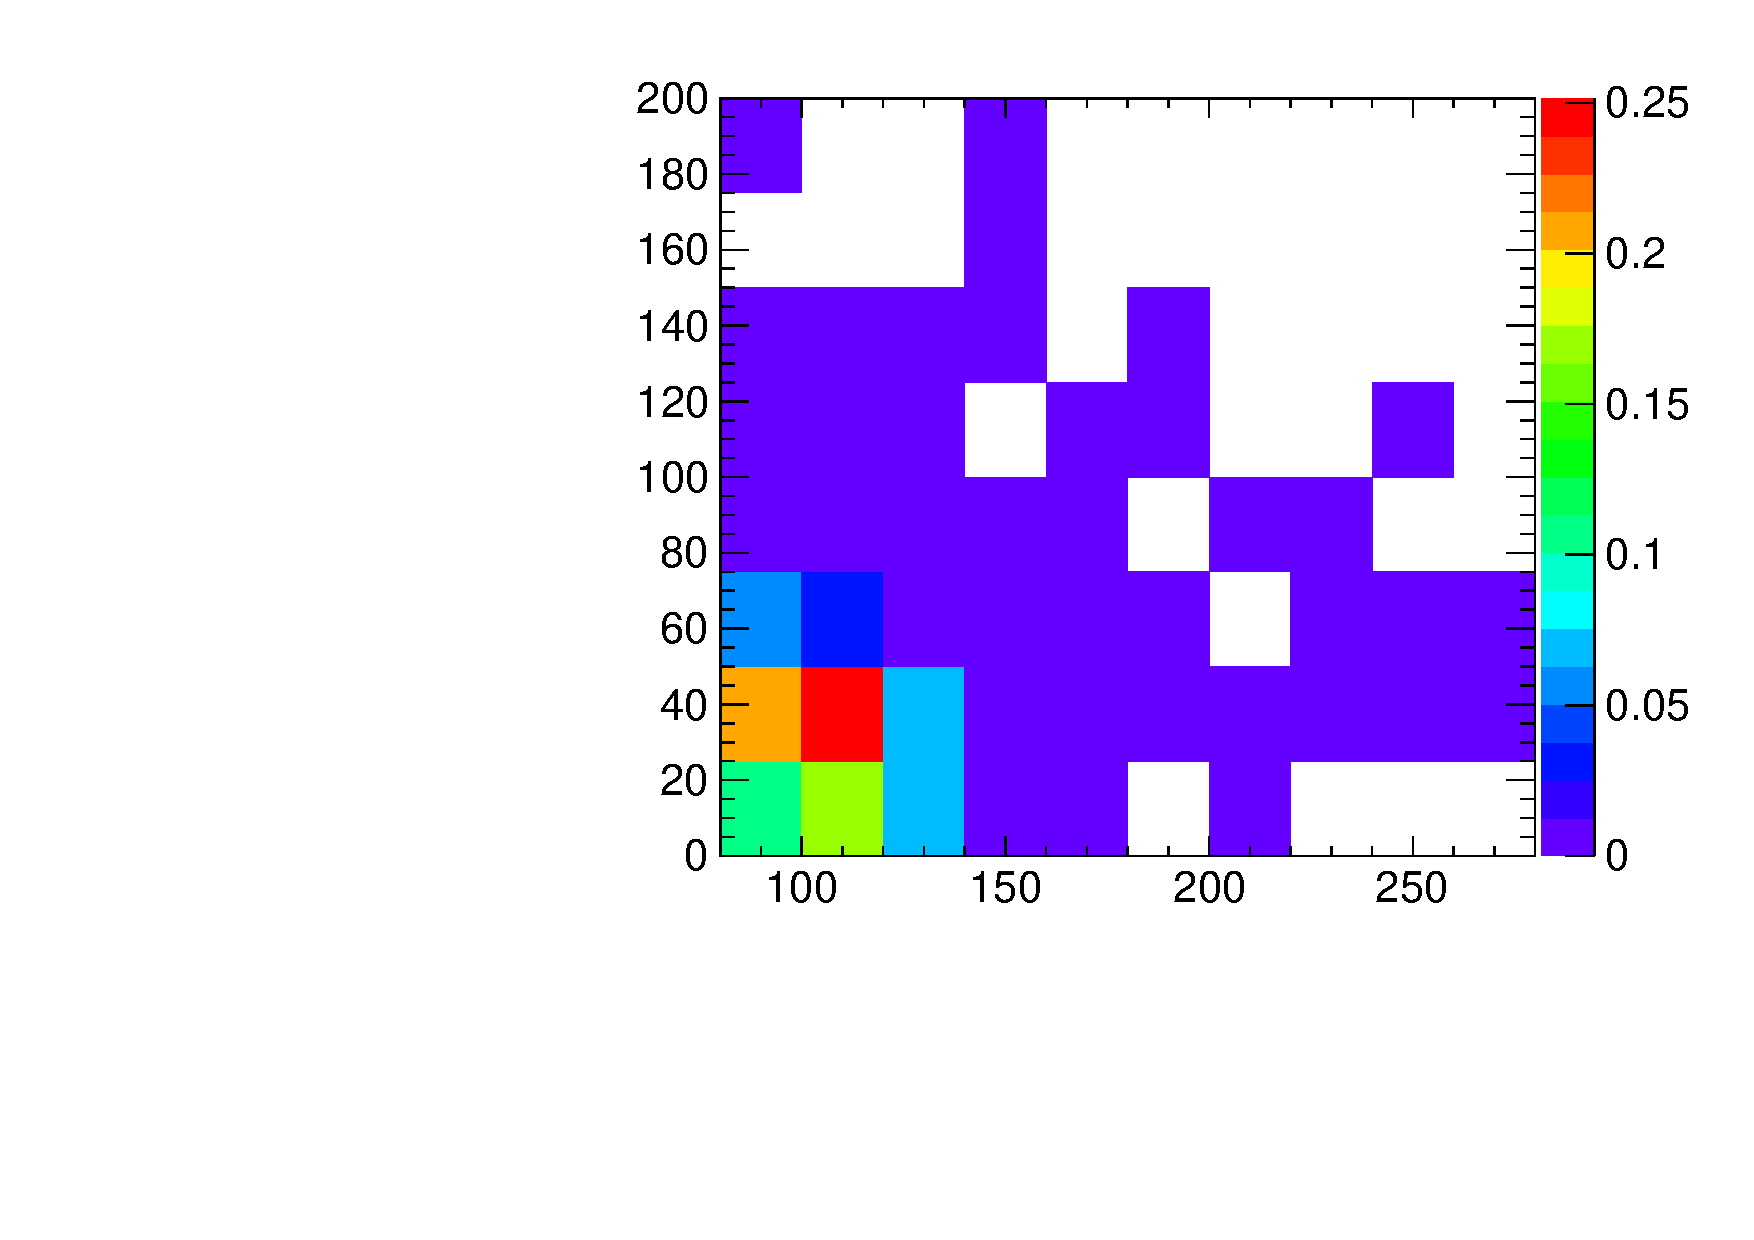
\includegraphics[width=.35\textwidth]{figures/templates/sig_2D_mH125_0j_of.pdf}
	}
	\subfigure[Signal statistical uncertainty]{
	\centering
	\label{subfig:template_signalerr_125}
		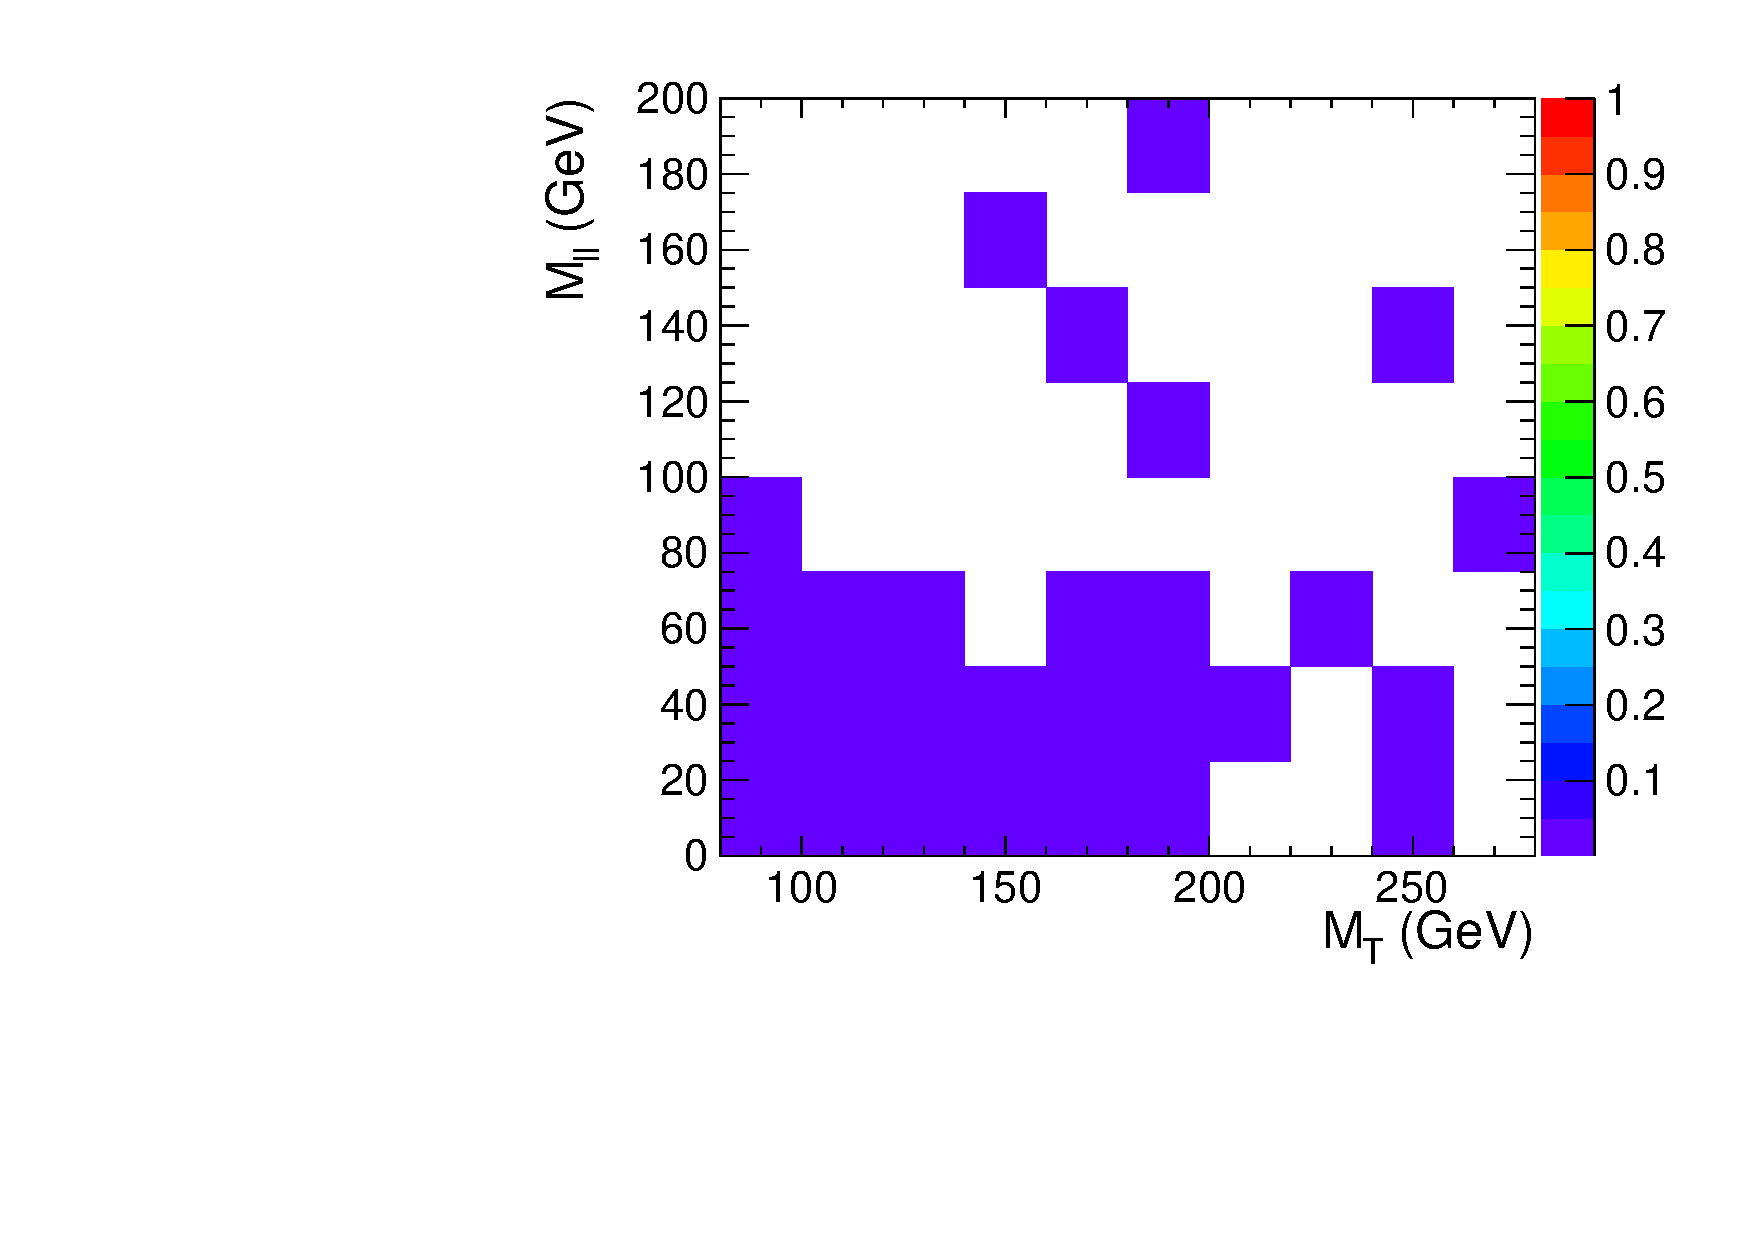
\includegraphics[width=.35\textwidth]{figures/templates/sigerr_2D_mH125_0j_of.pdf}
	}
	
	%
	\centering
	\subfigure[qqWW]{
	\centering
	\label{subfig:template_qqWW_125}
		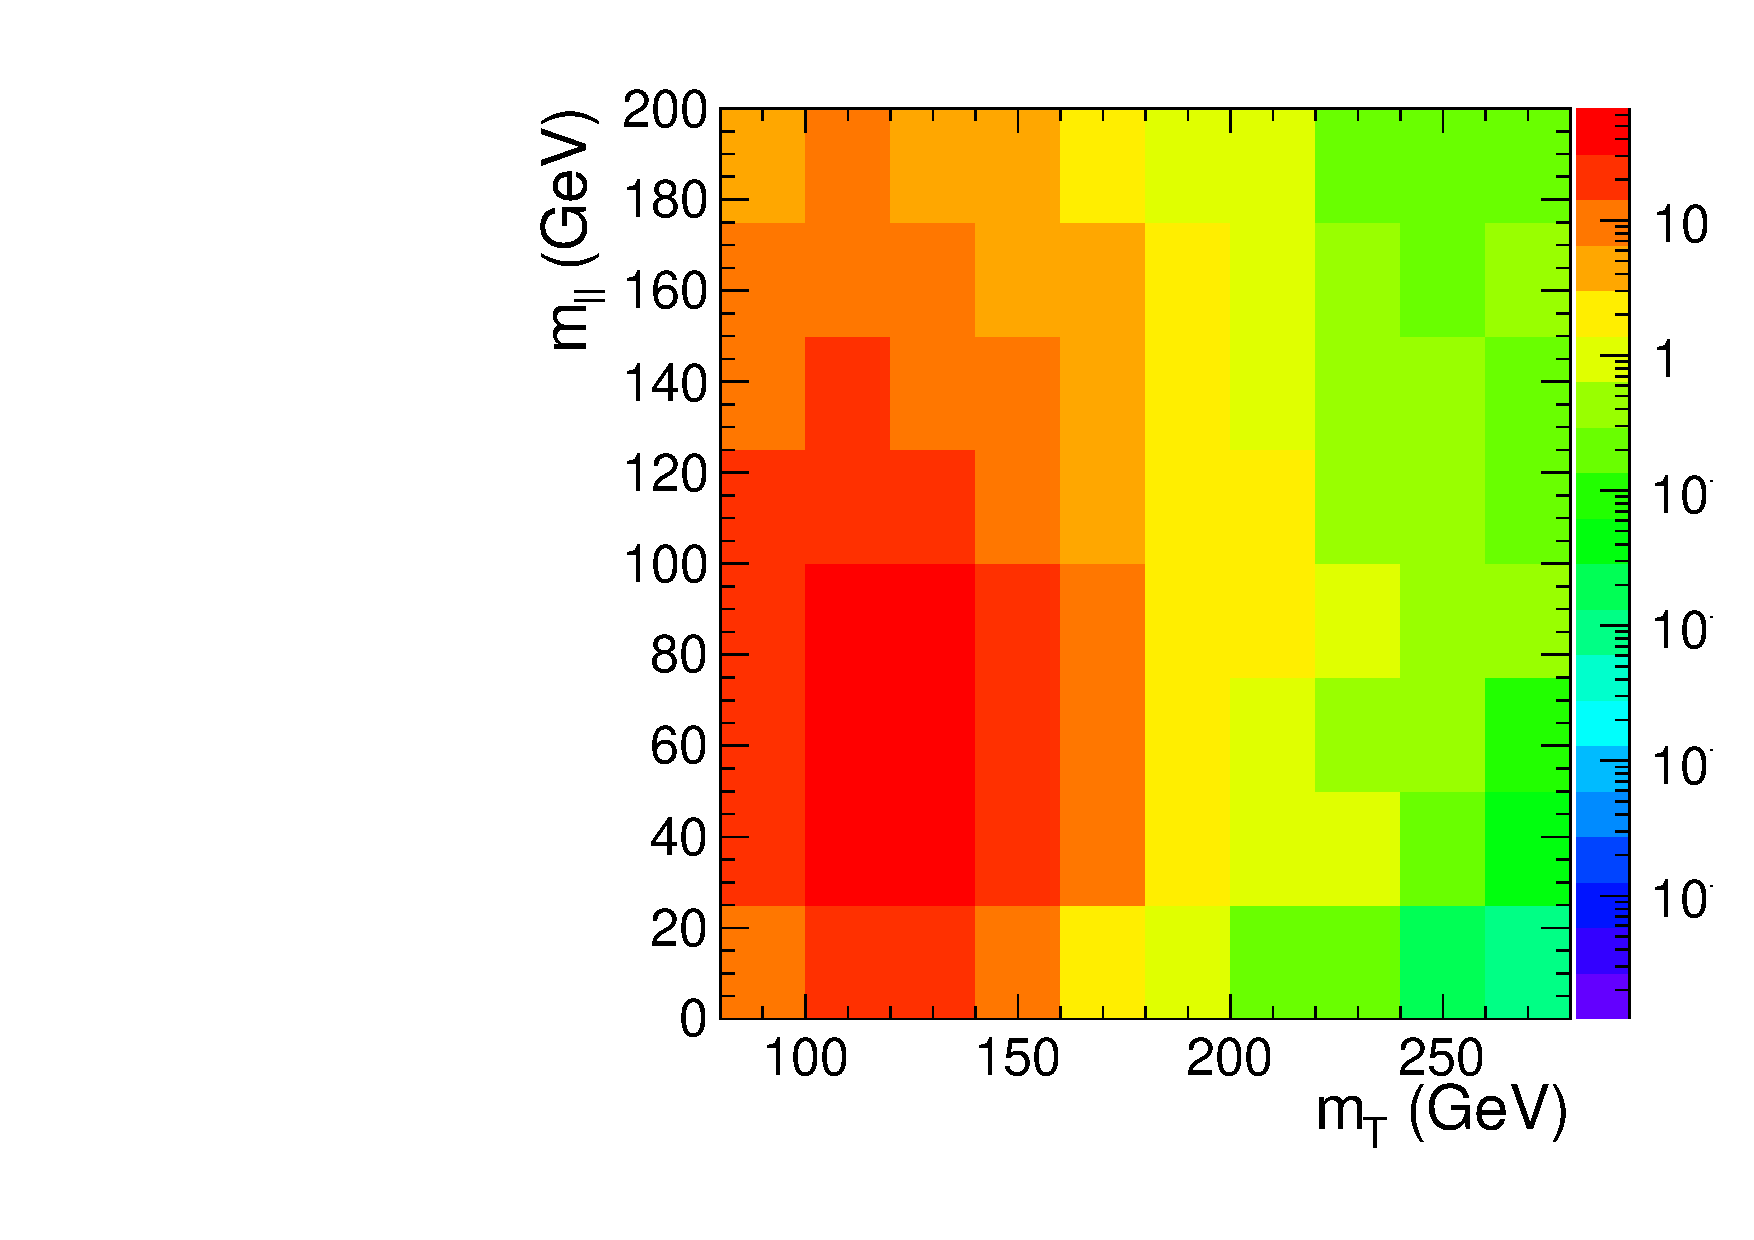
\includegraphics[width=.35\textwidth]{figures/templates/qqWW_2D_mH125_0j_of.pdf}
	}
	\subfigure[qqWW statistical uncertainty]{
	\centering
	\label{subfig:template_qqWWerr_125}
		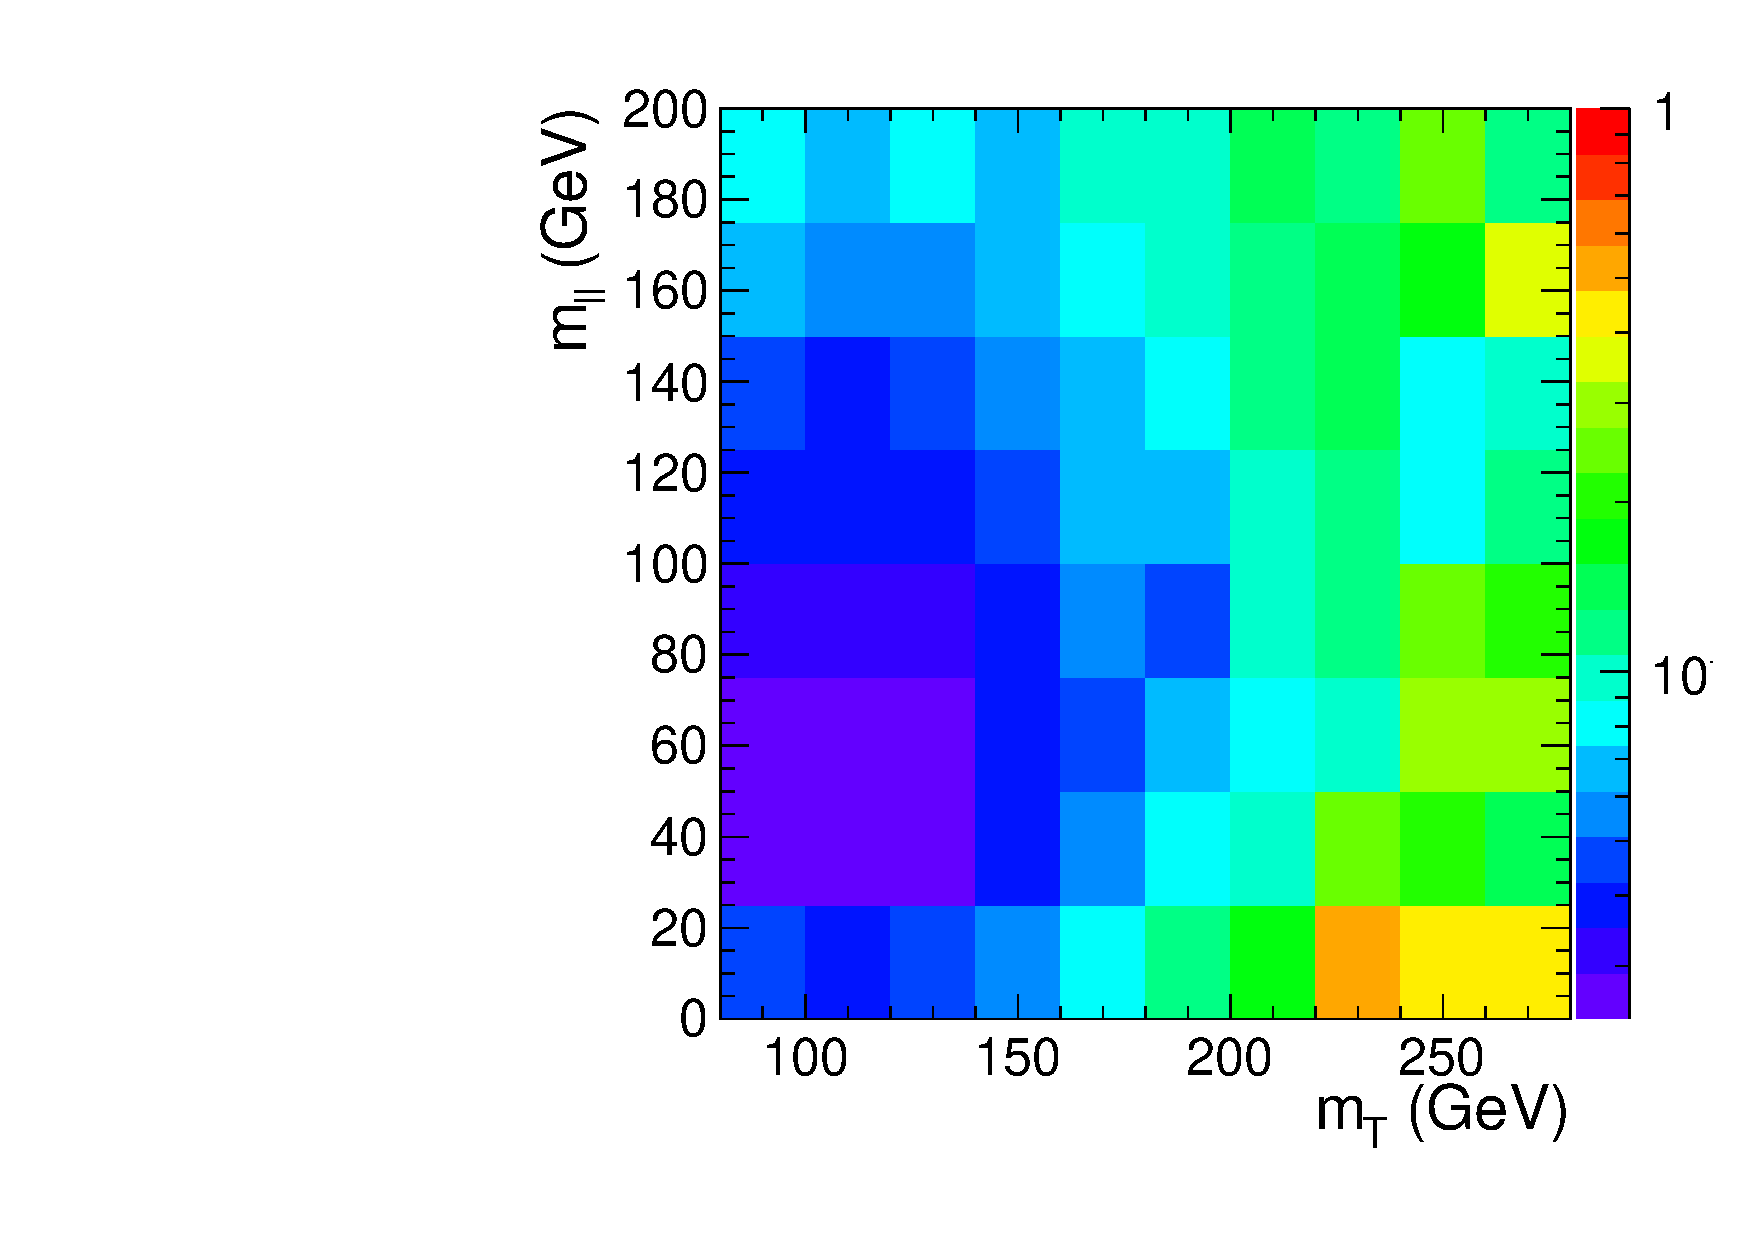
\includegraphics[width=.35\textwidth]{figures/templates/qqWWerr_2D_mH125_0j_of.pdf}
	}

	%
	\centering
	\subfigure[ggWW]{
	\centering
	\label{subfig:template_ggWW_125}
		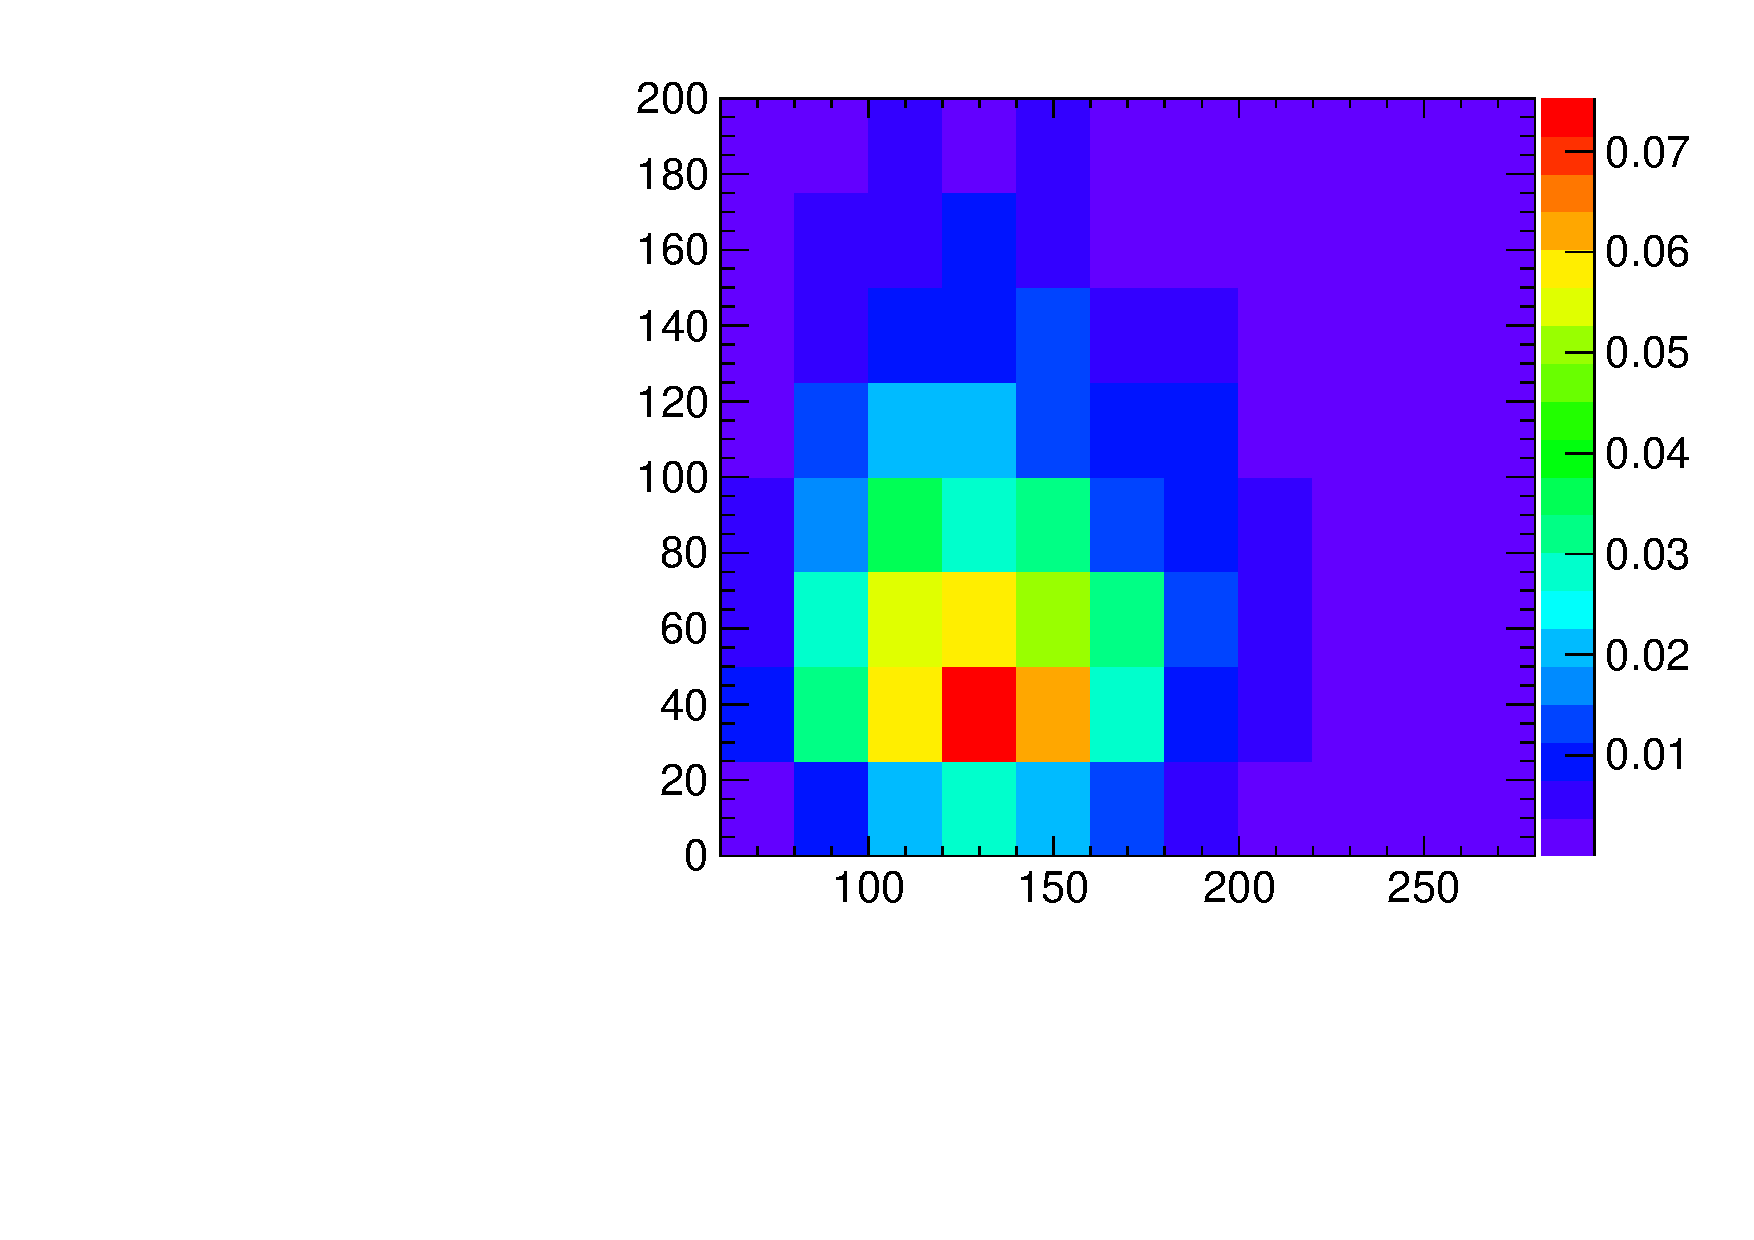
\includegraphics[width=.35\textwidth]{figures/templates/ggWW_2D_mH125_0j_of.pdf}
	}
	\subfigure[ggWW statistical uncertainty]{
	\centering
	\label{subfig:template_ggWWerr_125}
		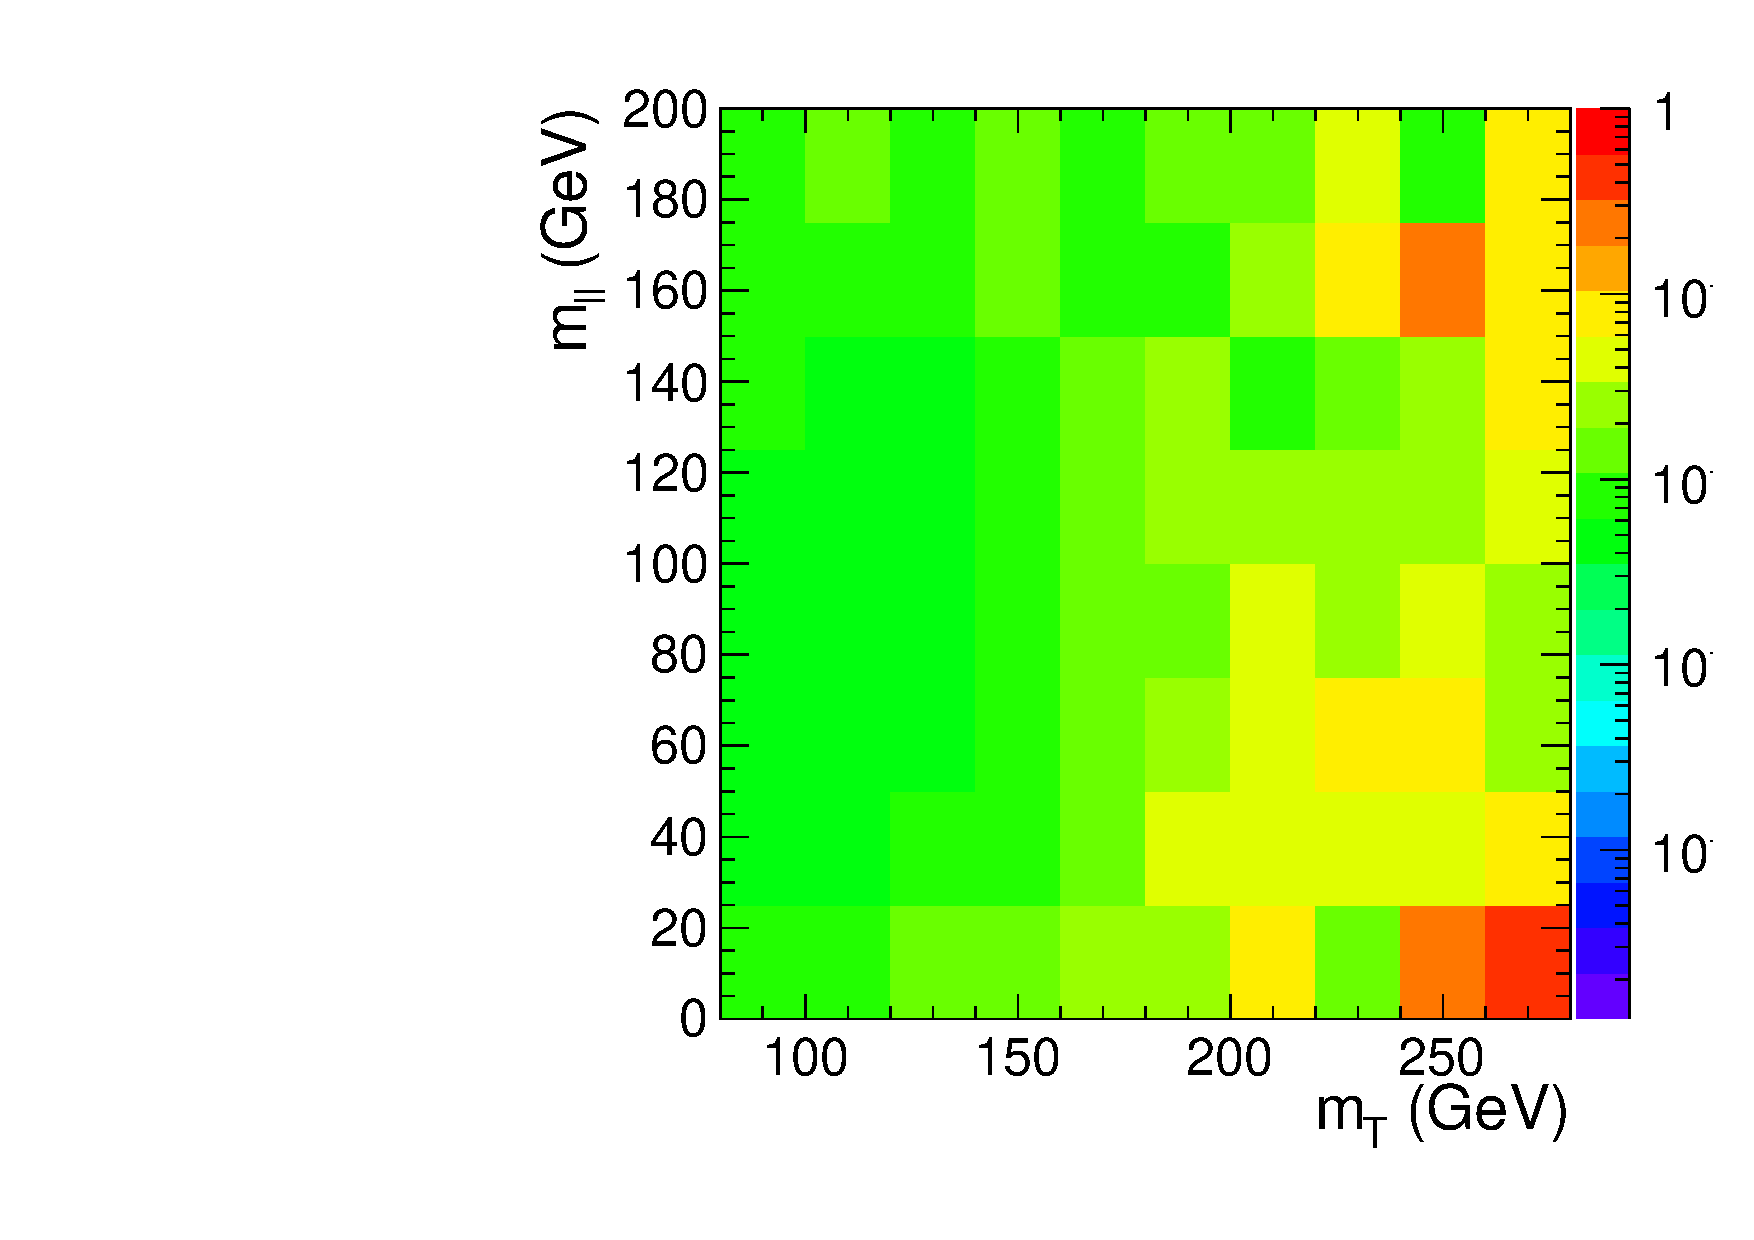
\includegraphics[width=.35\textwidth]{figures/templates/ggWWerr_2D_mH125_0j_of.pdf}
	}

	\caption{2D templates at \mHi = 125 \GeV in 0 jet bin} 
	\label{fig:templates_125_0j_1}

\end{figure}

\begin{figure}[!hbtp]
	
	%
	\centering
	\subfigure[Wjets]{
	\centering
	\label{subfig:template_Wjets_125}
		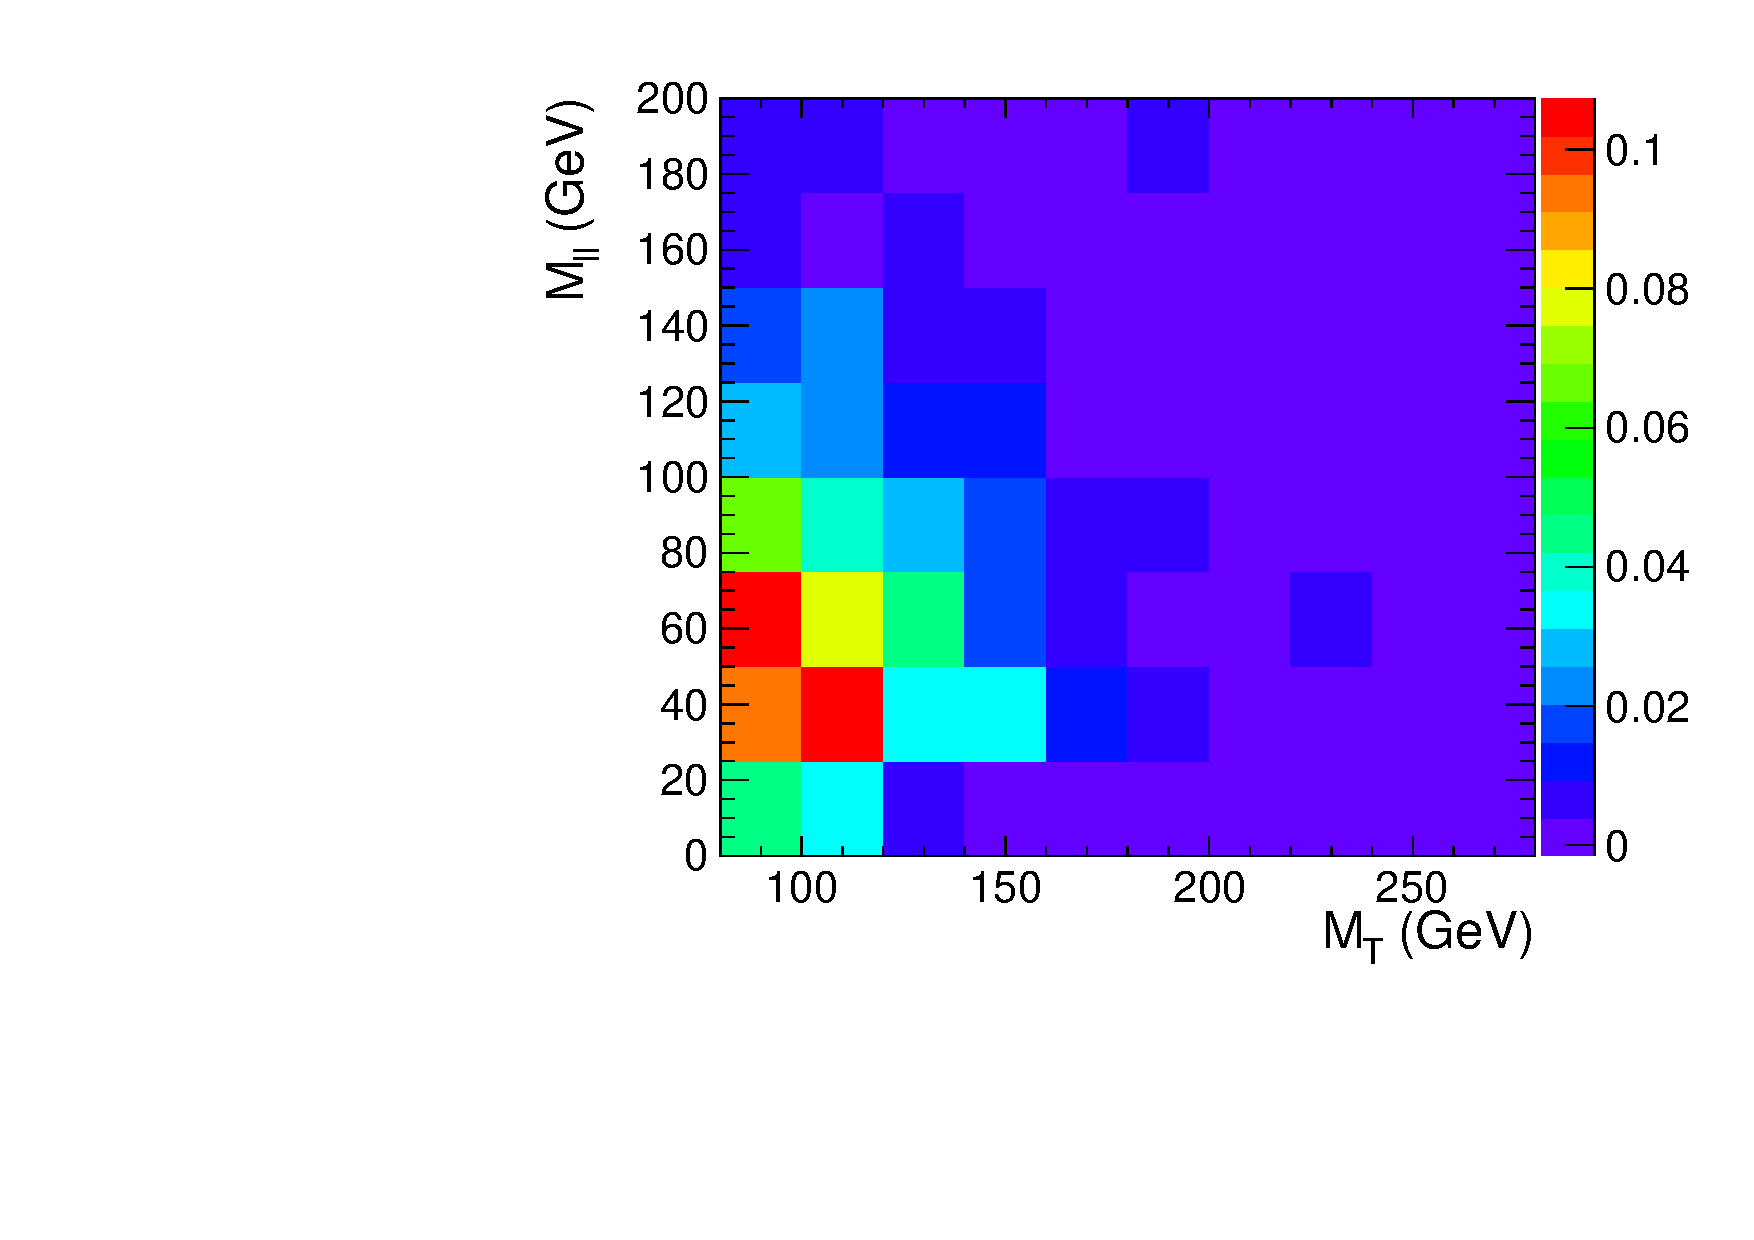
\includegraphics[width=.35\textwidth]{figures/templates/Wjets_2D_mH125_0j_of.pdf}
	}
	\subfigure[Wjets statistical uncertainty]{
	\centering
	\label{subfig:template_Wjetserr_125}
		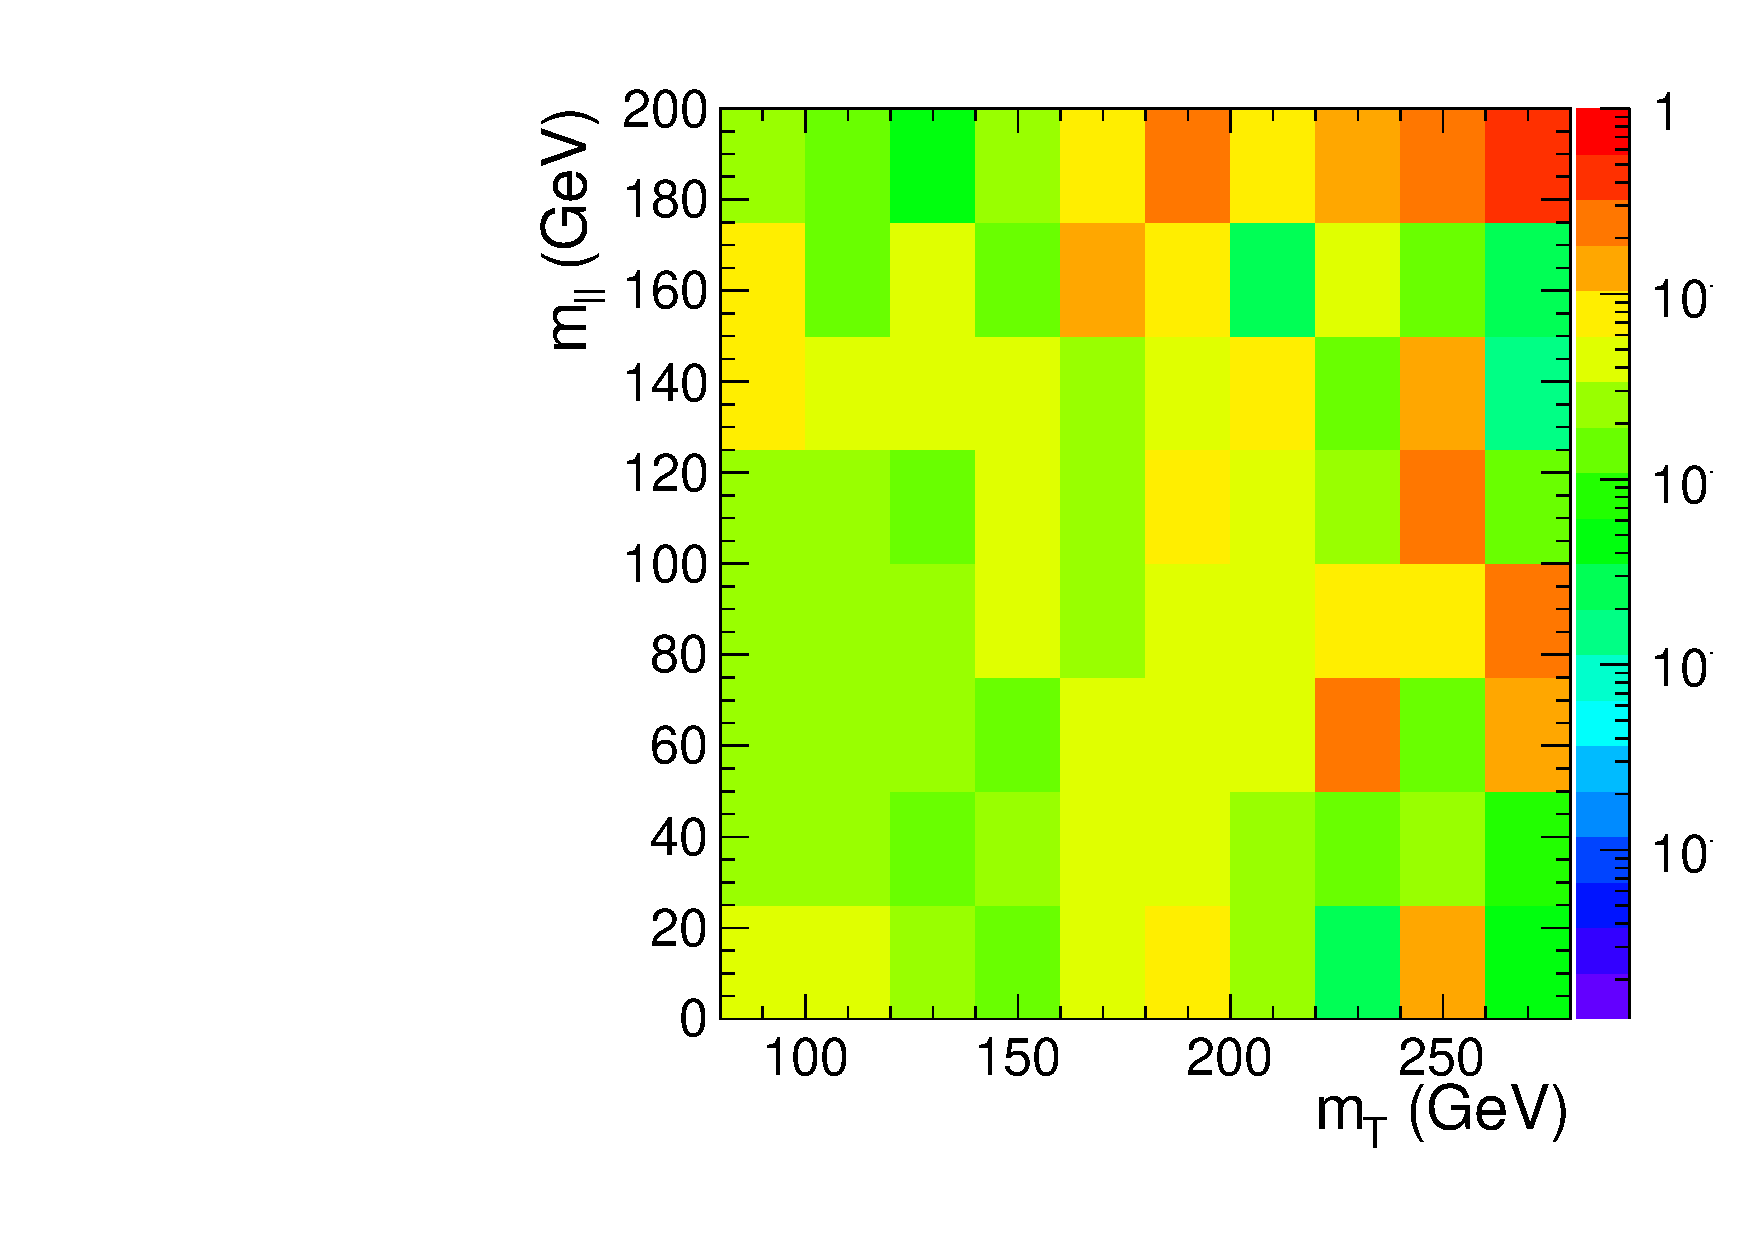
\includegraphics[width=.35\textwidth]{figures/templates/Wjetserr_2D_mH125_0j_of.pdf}
	}
	
	%
	\centering
	\subfigure[Top]{
	\centering
	\label{subfig:template_Top_125}
		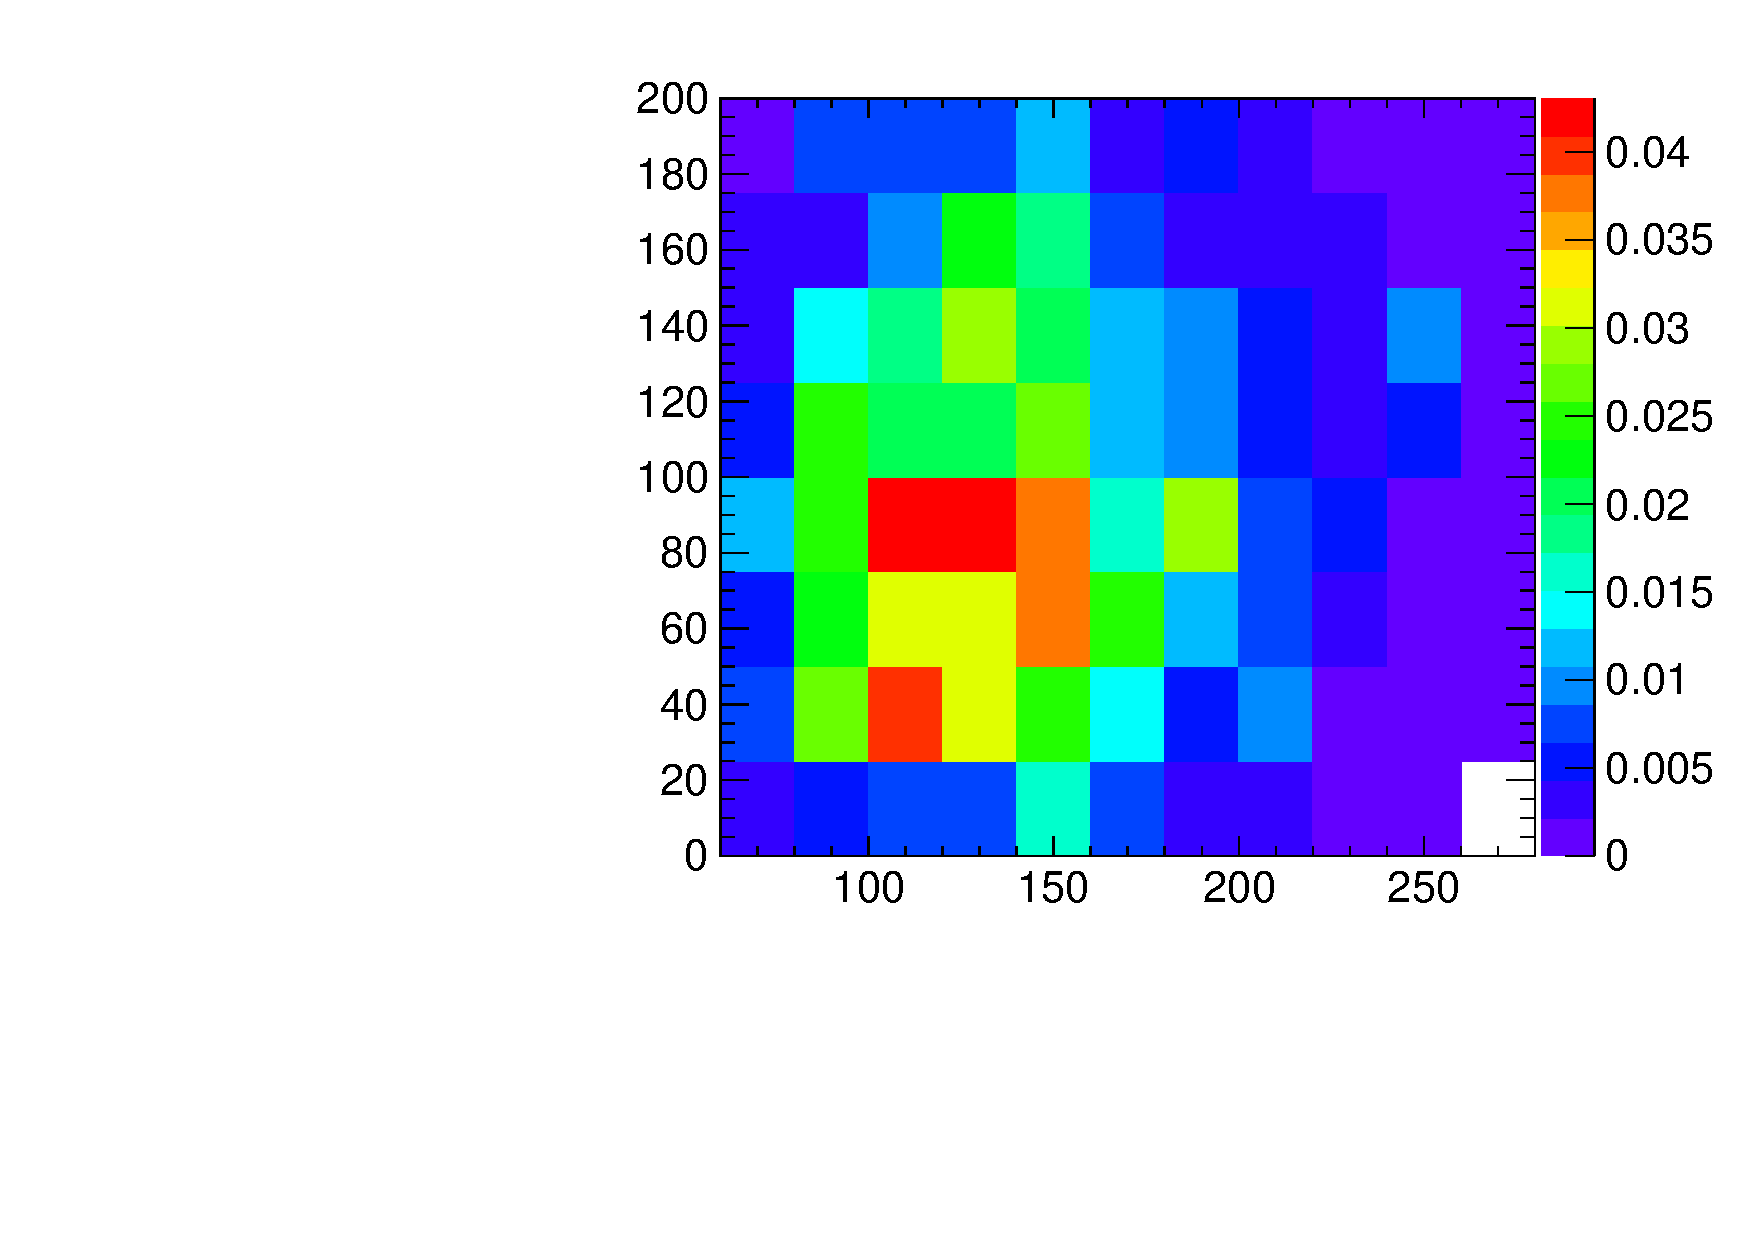
\includegraphics[width=.35\textwidth]{figures/templates/Top_2D_mH125_0j_of.pdf}
	}
	\subfigure[Top statistical uncertainty]{
	\centering
	\label{subfig:template_Toperr_125}
		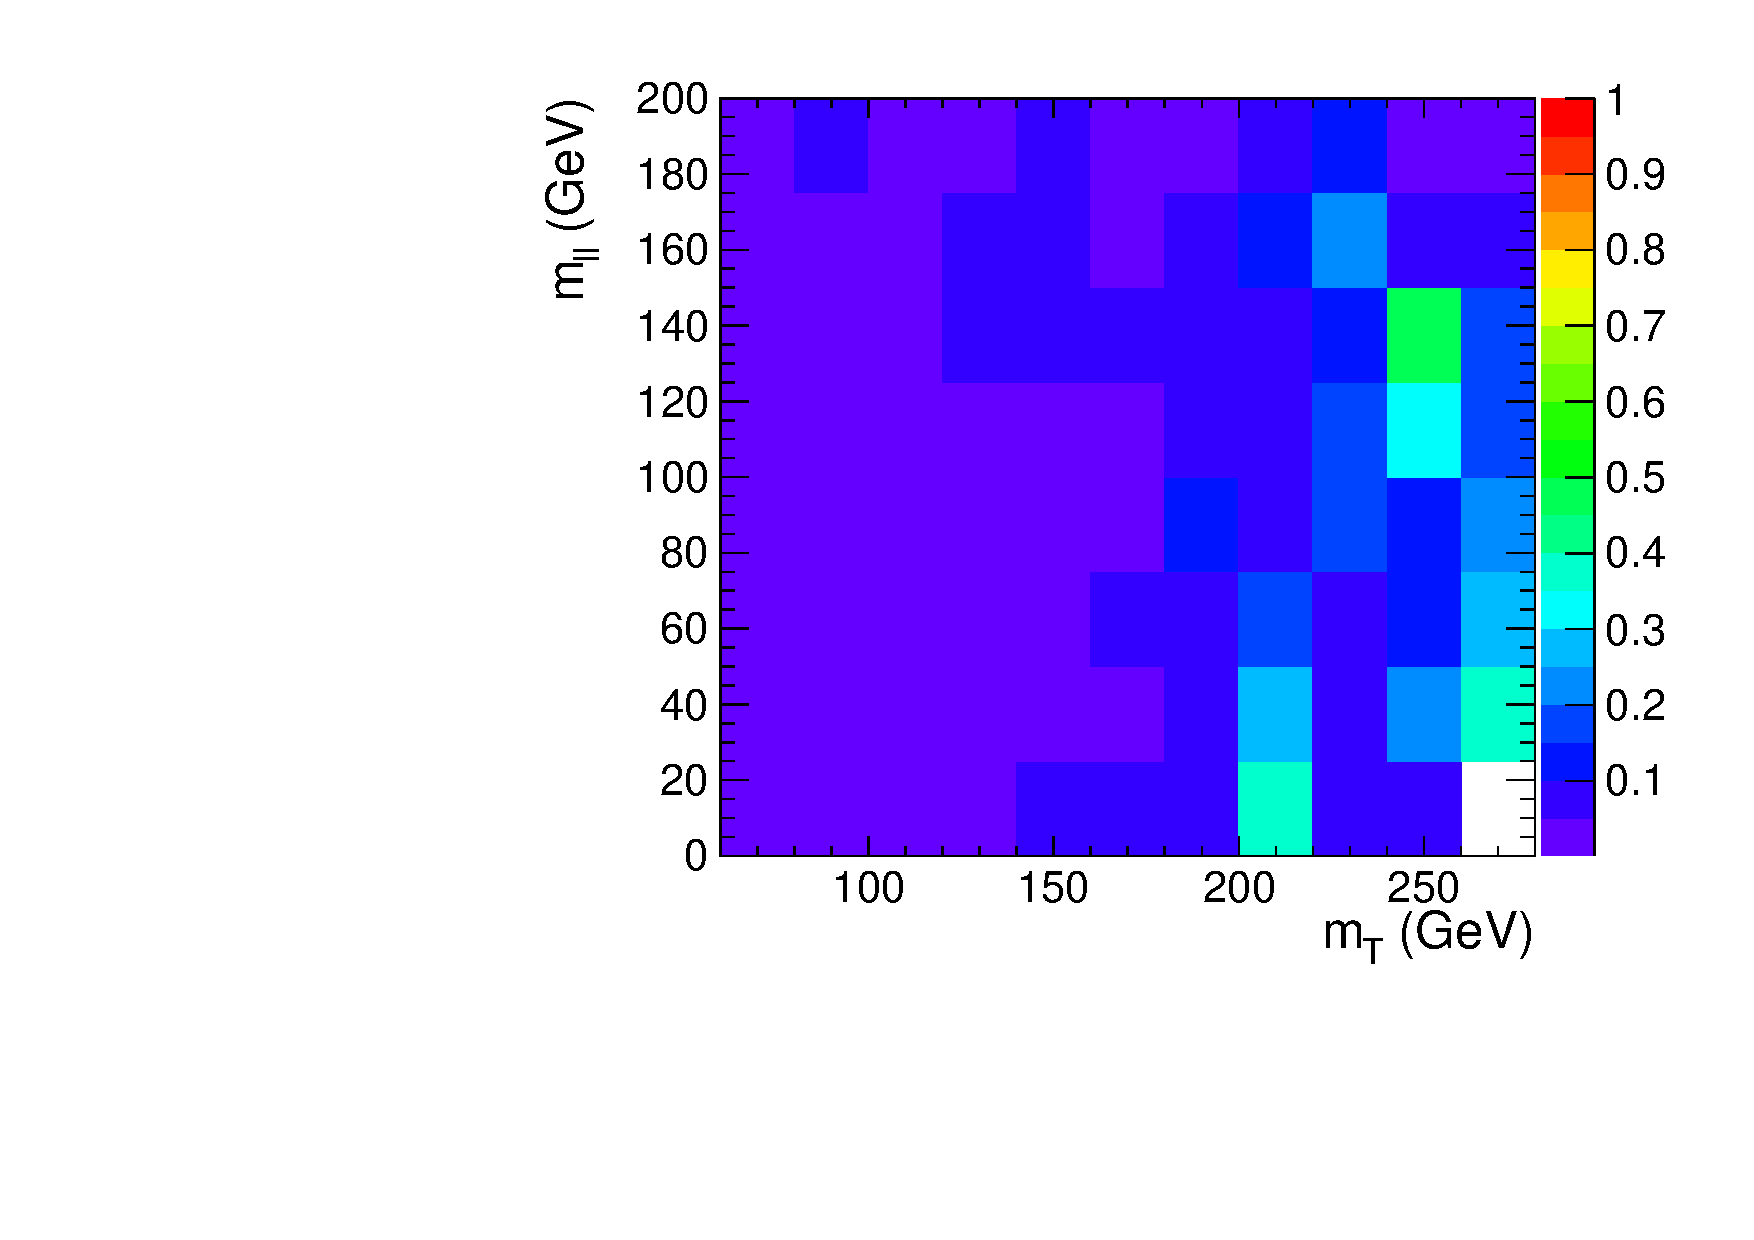
\includegraphics[width=.35\textwidth]{figures/templates/Toperr_2D_mH125_0j_of.pdf}
	}

	%
	\centering
	\subfigure[VV]{
	\centering
	\label{subfig:template_VV_125}
		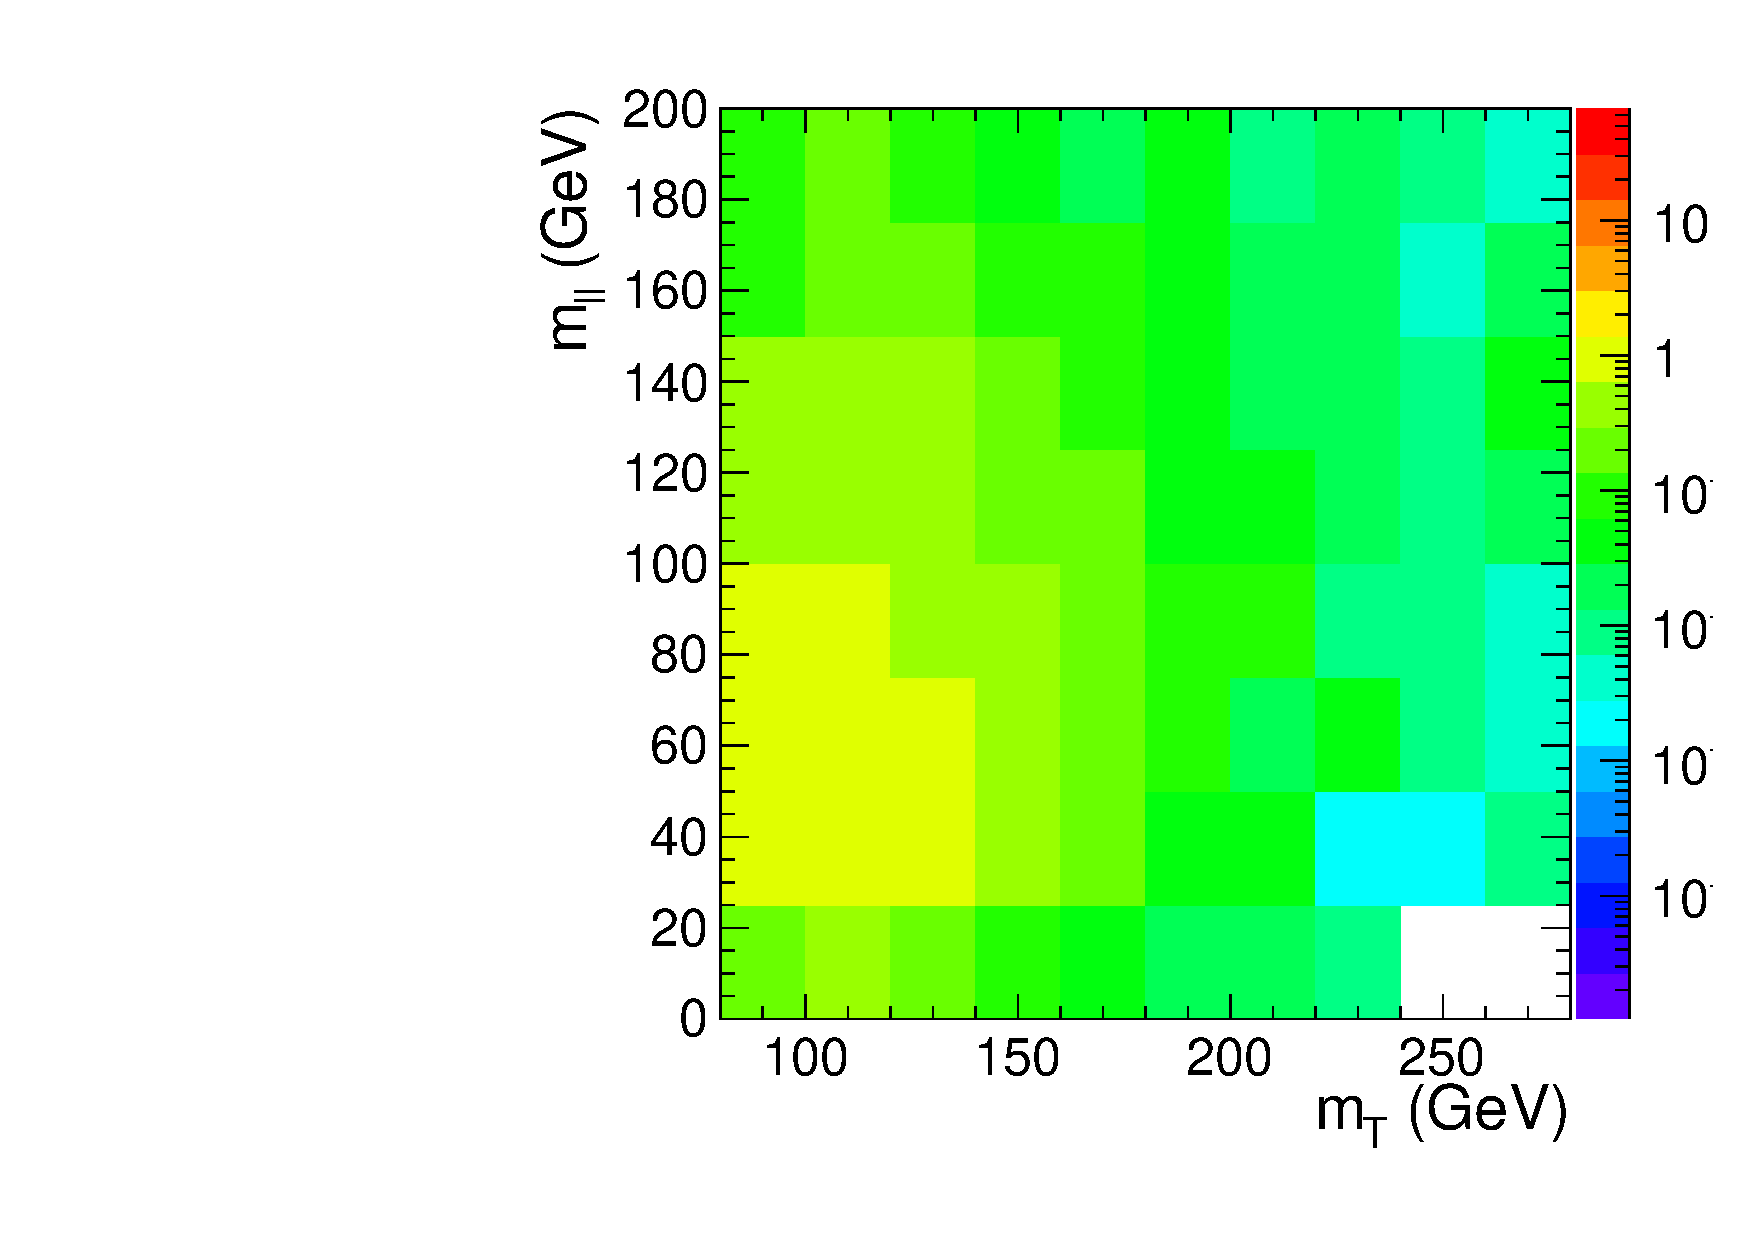
\includegraphics[width=.35\textwidth]{figures/templates/VV_2D_mH125_0j_of.pdf}
	}
	\subfigure[VV statistical uncertainty]{
	\centering
	\label{subfig:template_VVerr_125}
		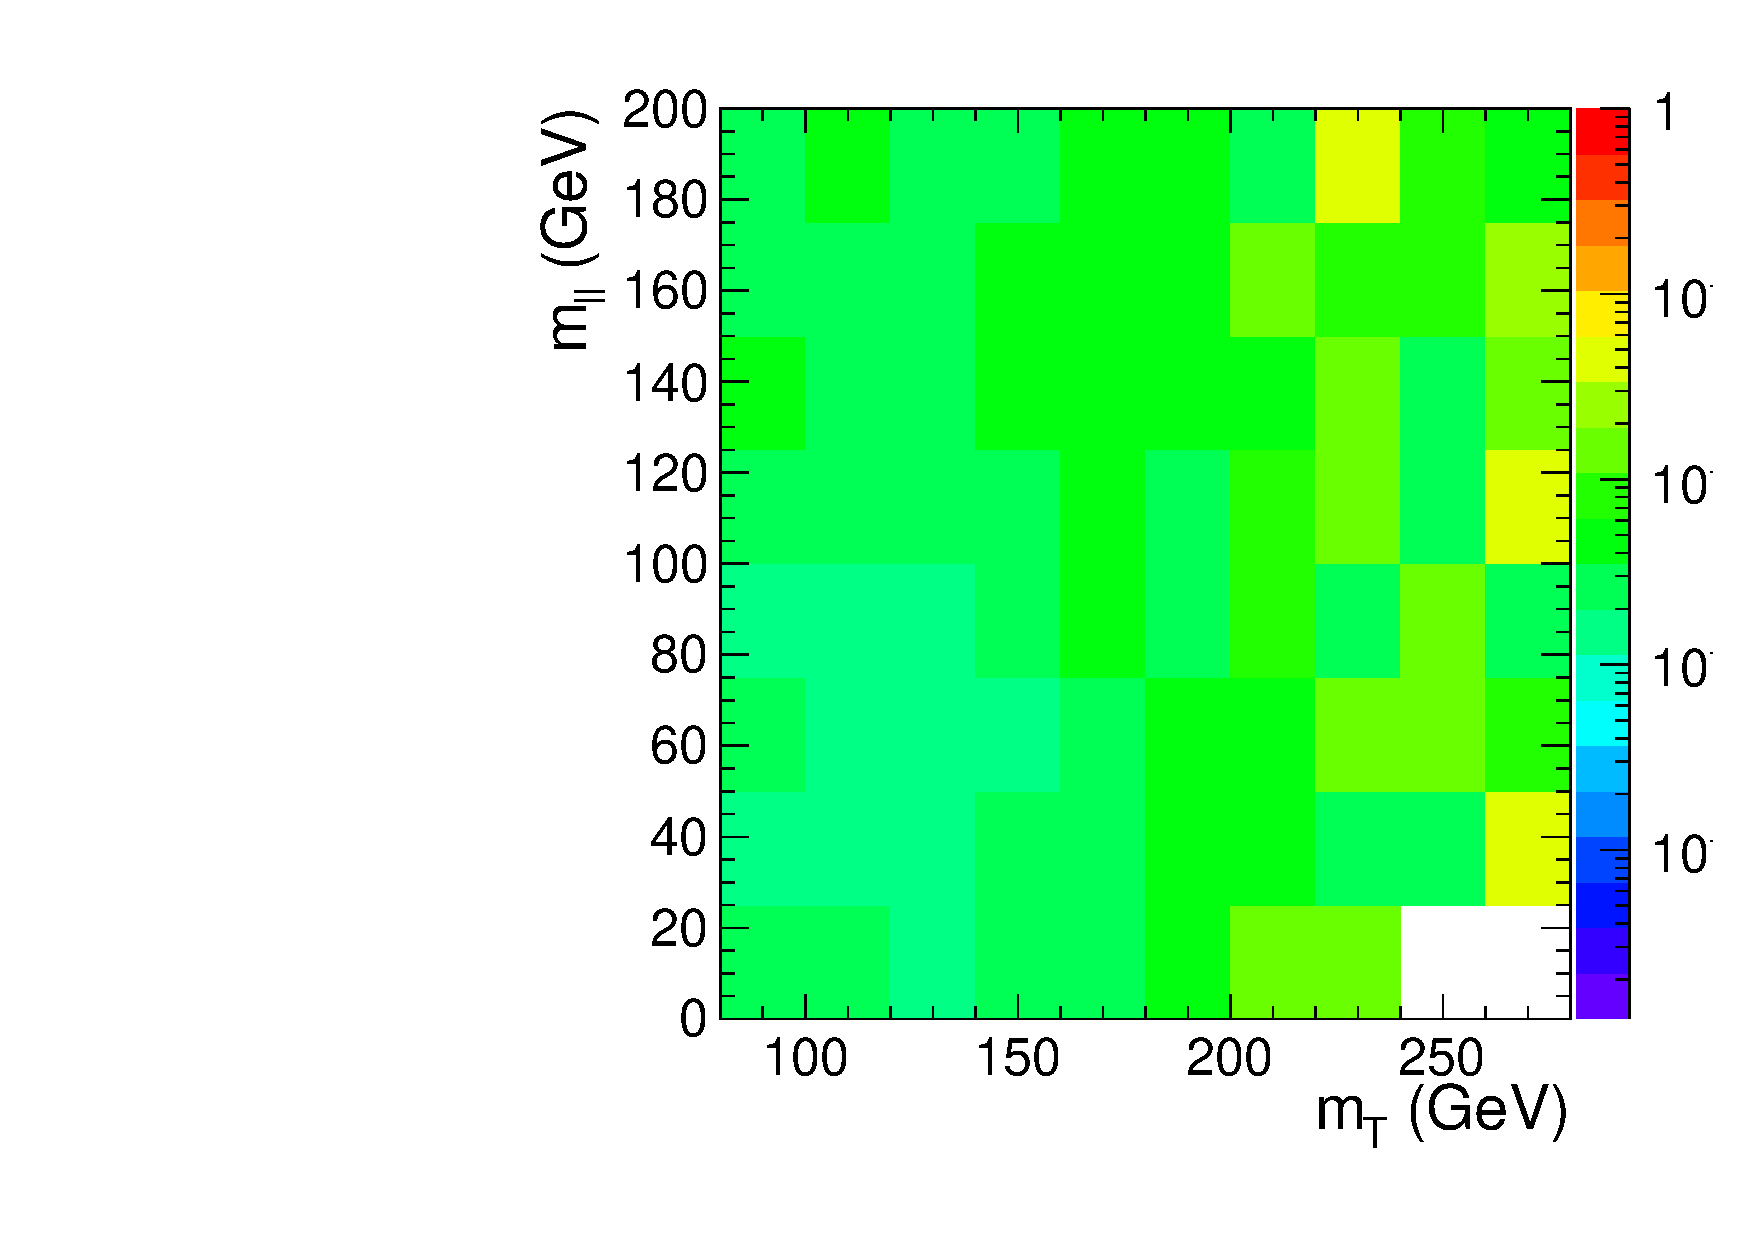
\includegraphics[width=.35\textwidth]{figures/templates/VVerr_2D_mH125_0j_of.pdf}
	}

	\caption{2D templates at \mHi = 125 \GeV in 0jet bin.} 
	\label{fig:templates_125_0j_2}

\end{figure}

\begin{figure}[!hbtp]
	
	%
	\centering
	\subfigure[Zjets]{
	\centering
	\label{subfig:template_Zjets_125}
		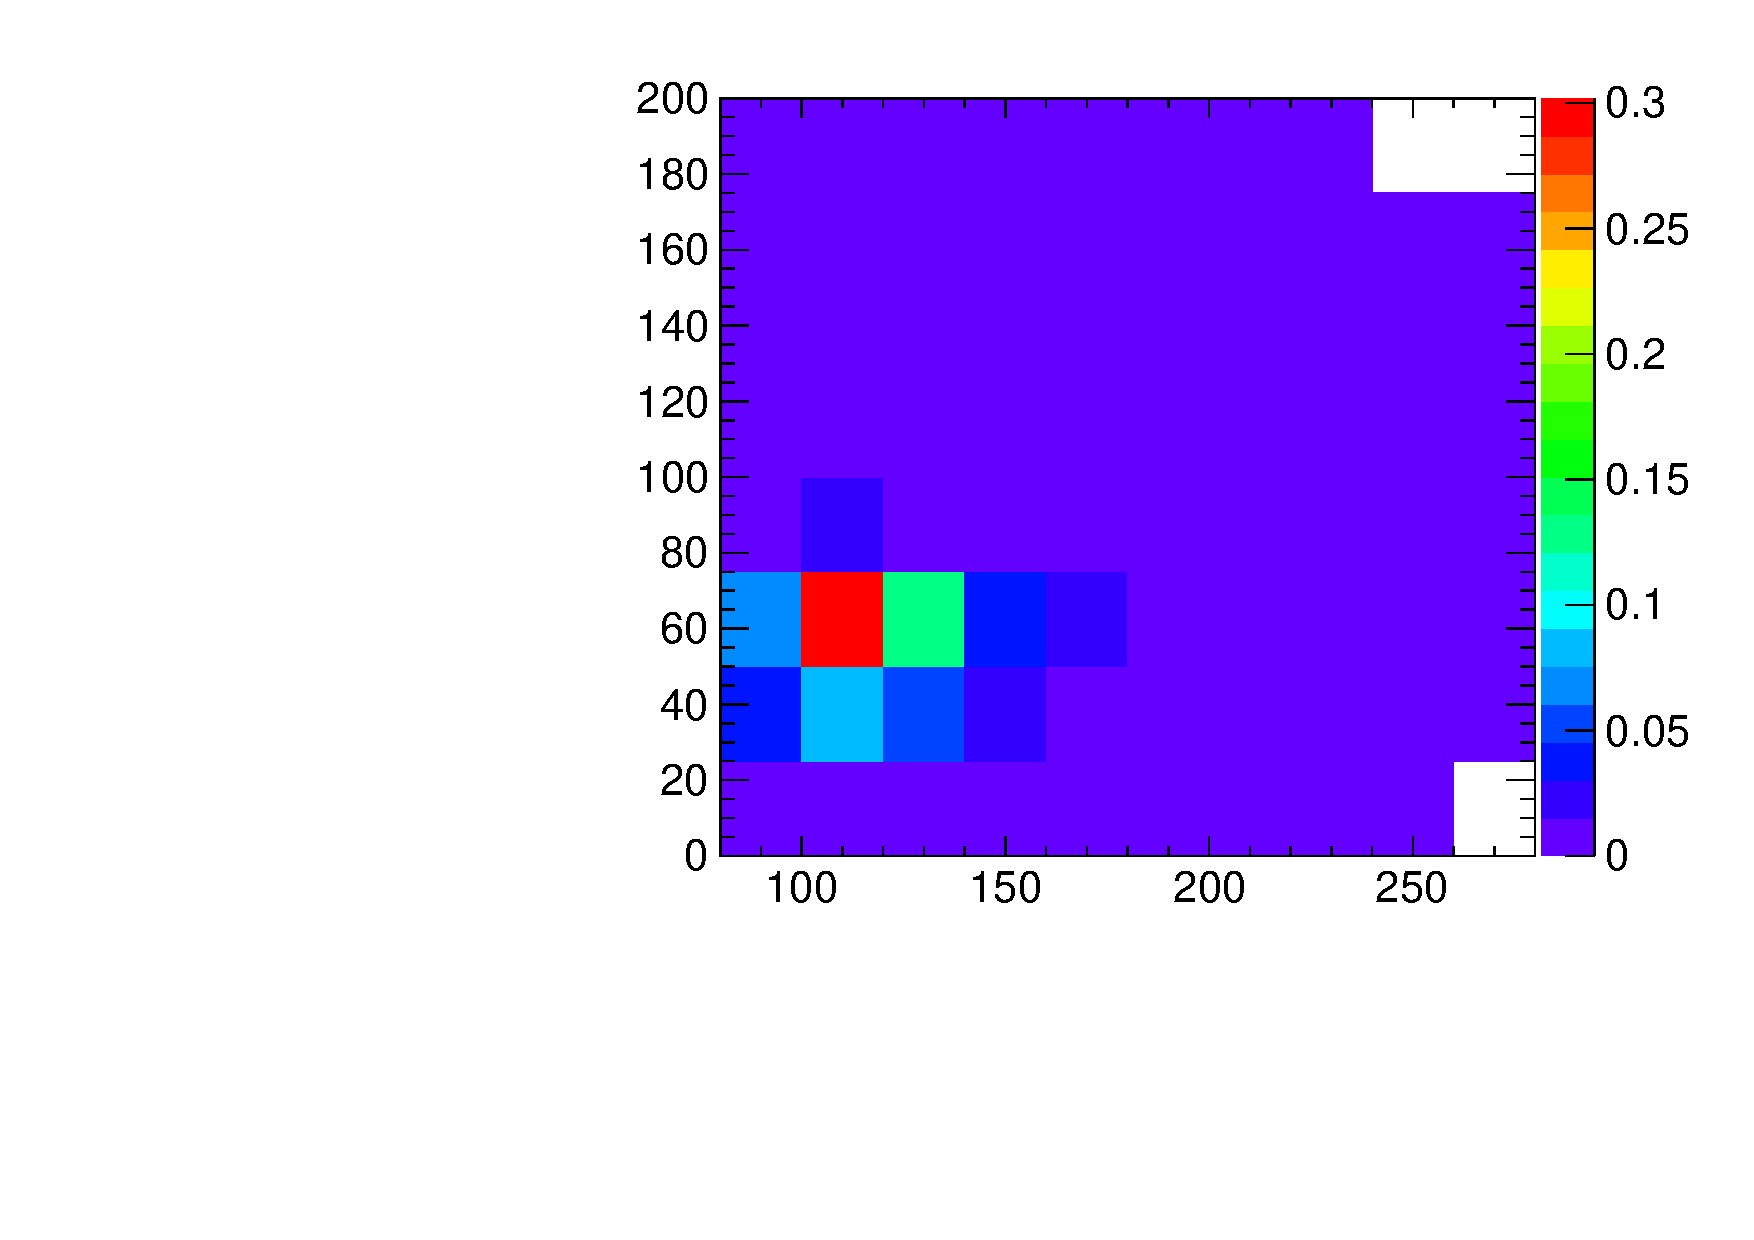
\includegraphics[width=.35\textwidth]{figures/templates/Zjets_2D_mH125_0j_of.pdf}
	}
	\subfigure[Zjets statistical uncertainty]{
	\centering
	\label{subfig:template_Zjetserr_125}
		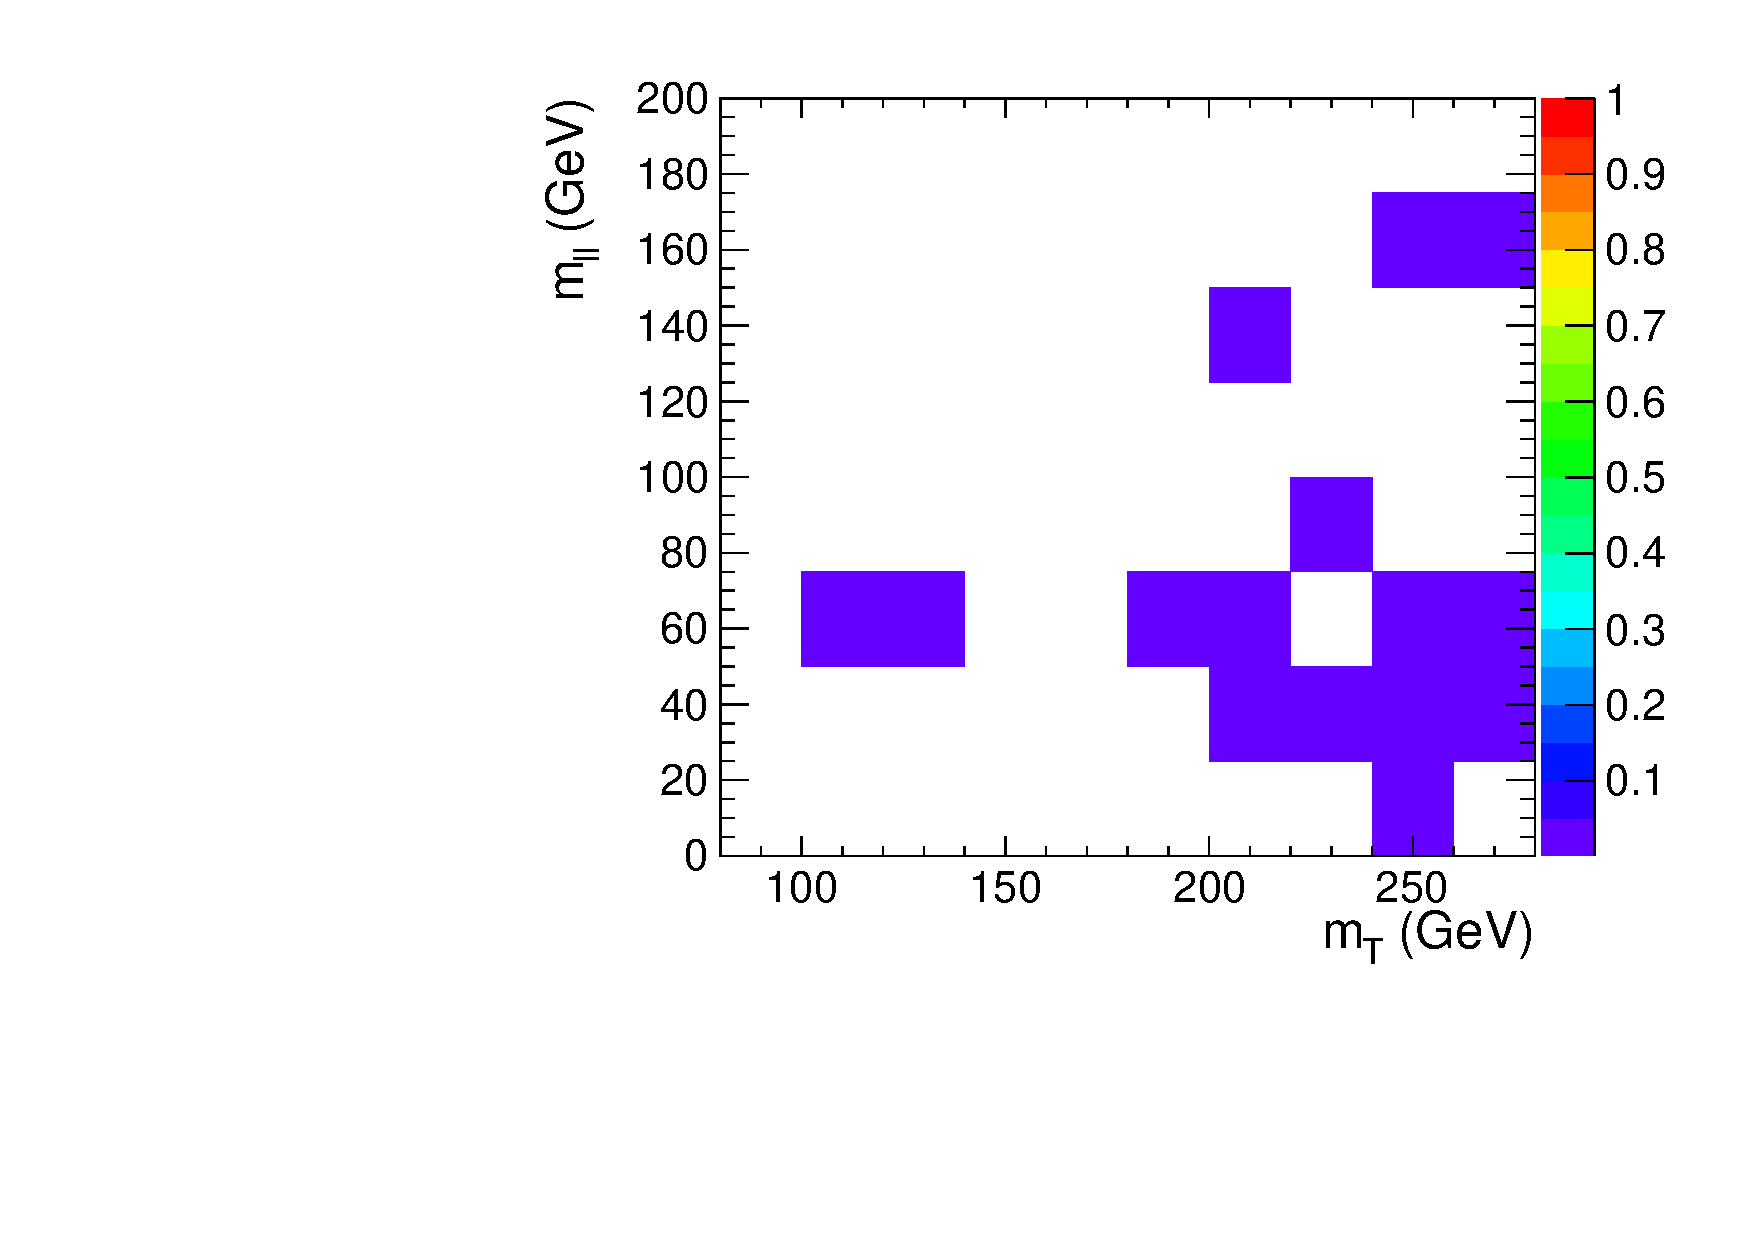
\includegraphics[width=.35\textwidth]{figures/templates/Zjetserr_2D_mH125_0j_of.pdf}
	}

	%
	\centering
	\subfigure[Wgamma]{
	\centering
	\label{subfig:template_Wgamma_125}
		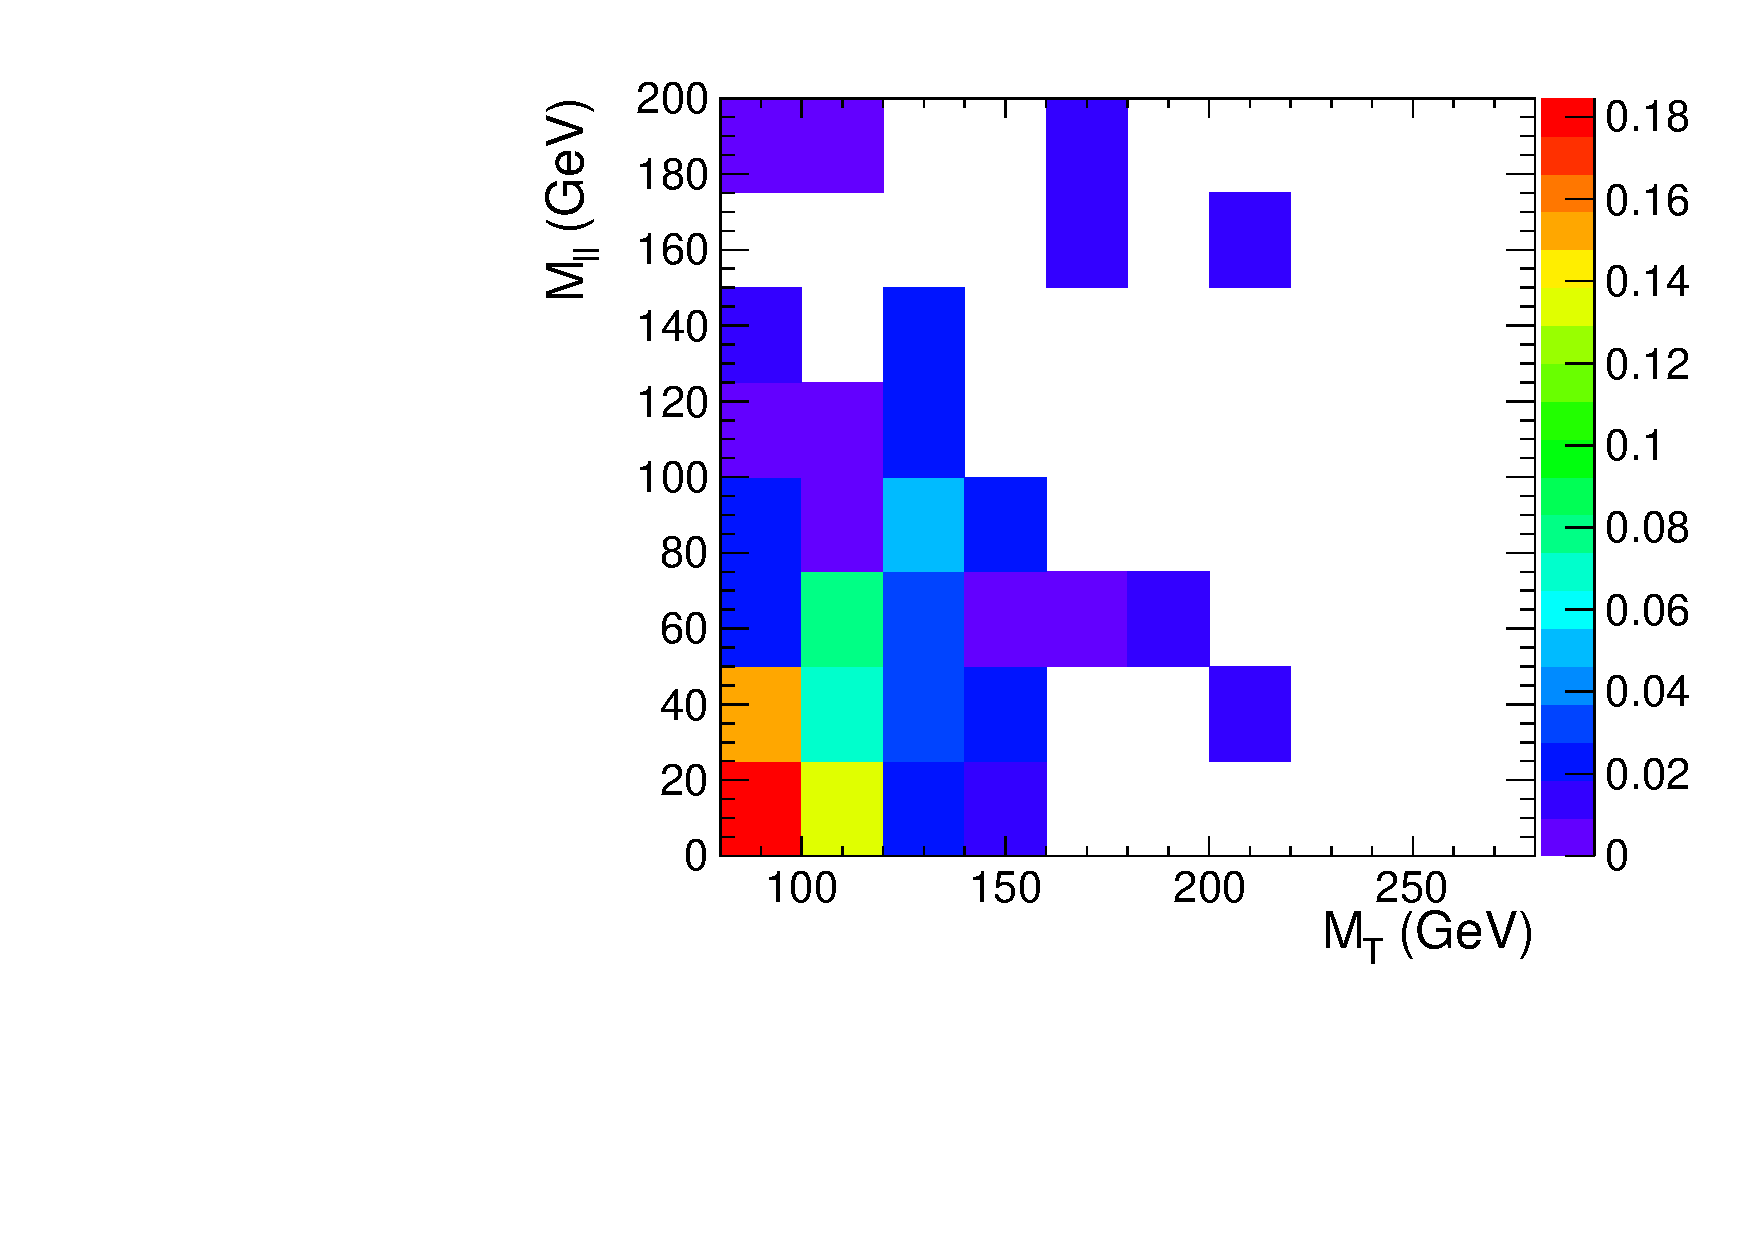
\includegraphics[width=.35\textwidth]{figures/templates/Wgamma_2D_mH125_0j_of.pdf}
	}
	\subfigure[Wgamma statistical uncertainty]{
	\centering
	\label{subfig:template_Wgammaerr_125}
		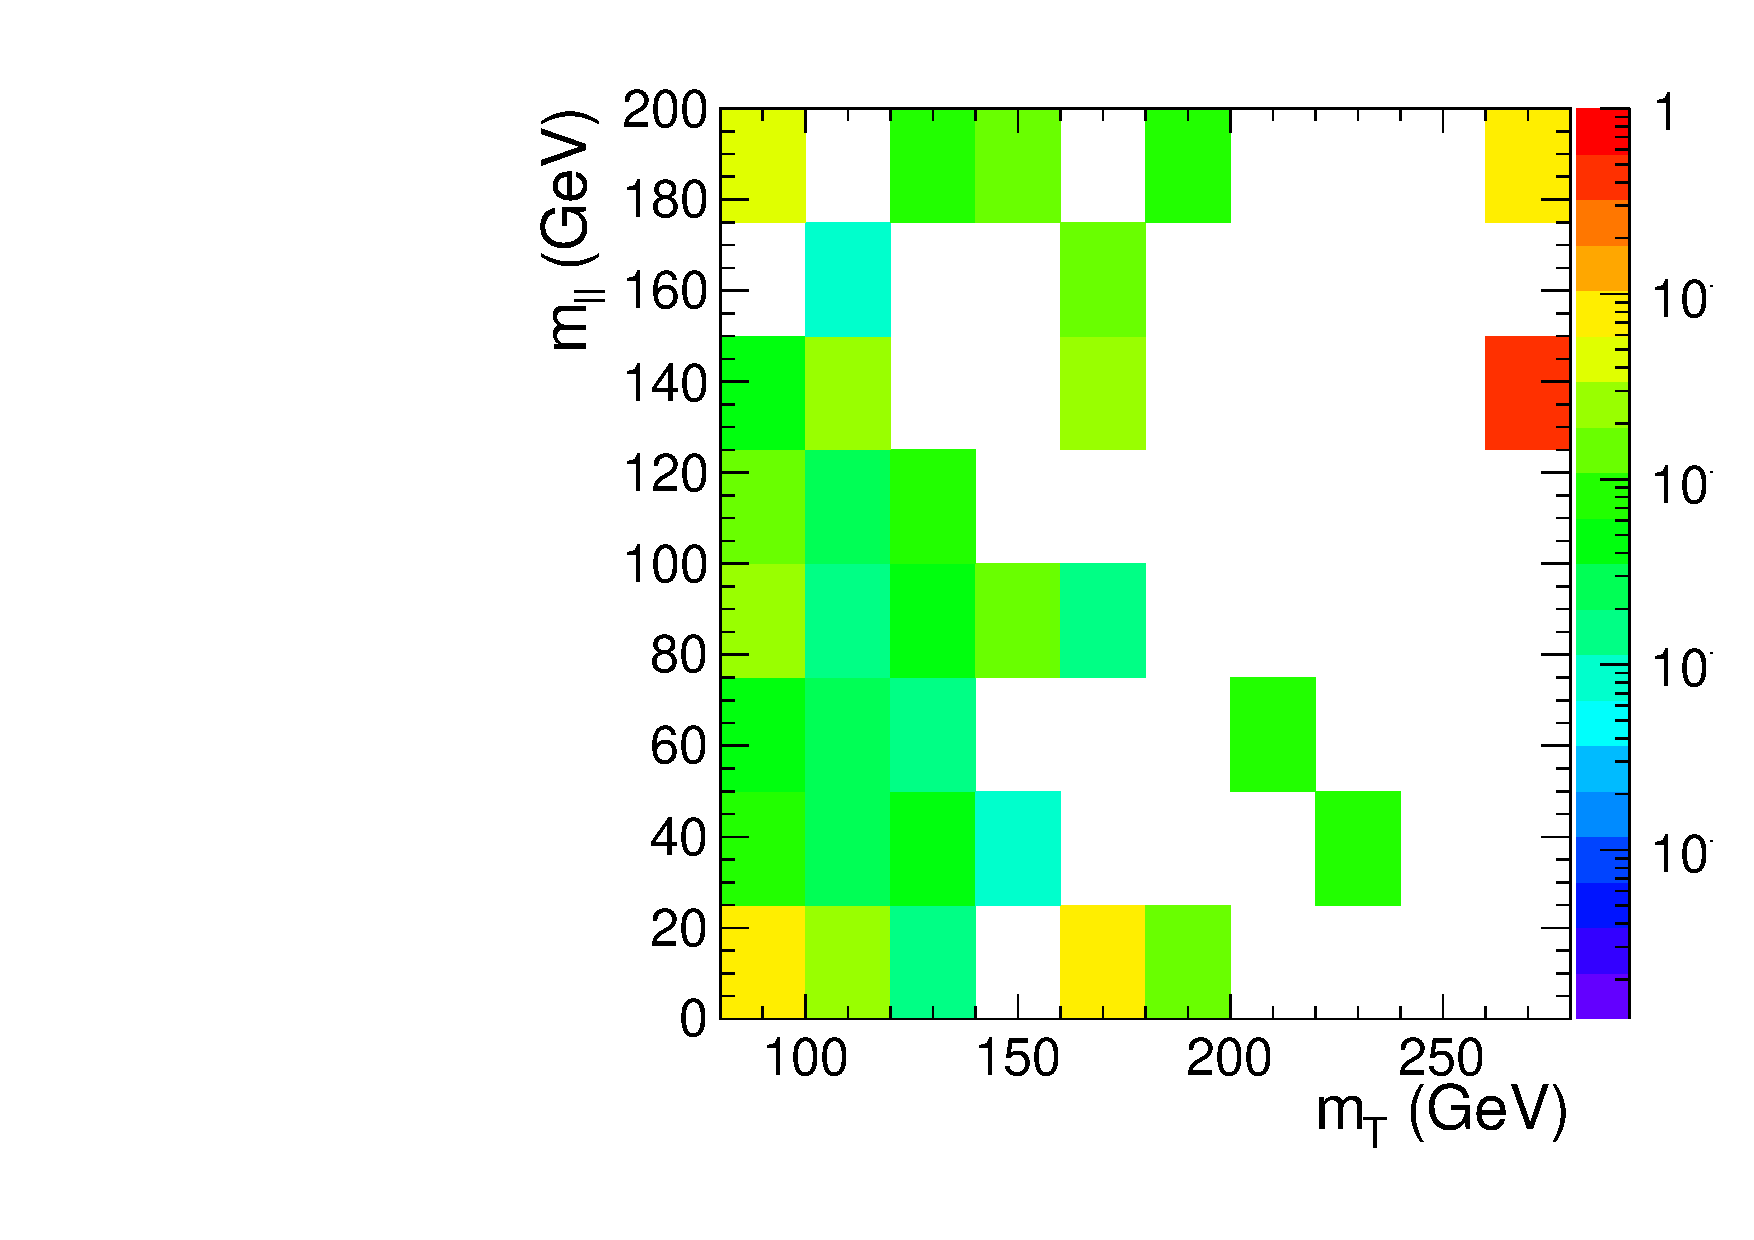
\includegraphics[width=.35\textwidth]{figures/templates/Wgammaerr_2D_mH125_0j_of.pdf}
	}

	\caption{2D templates at \mHi = 125 \GeV in 0jet bin.} 
	\label{fig:templates_125_0j_3}

\end{figure} 

\begin{figure}[!hbtp]
	
	%
	\centering
	\subfigure[Stacked unrolled template linear]{
	\centering
	\label{subfig:template_unroll_stack_lin}
		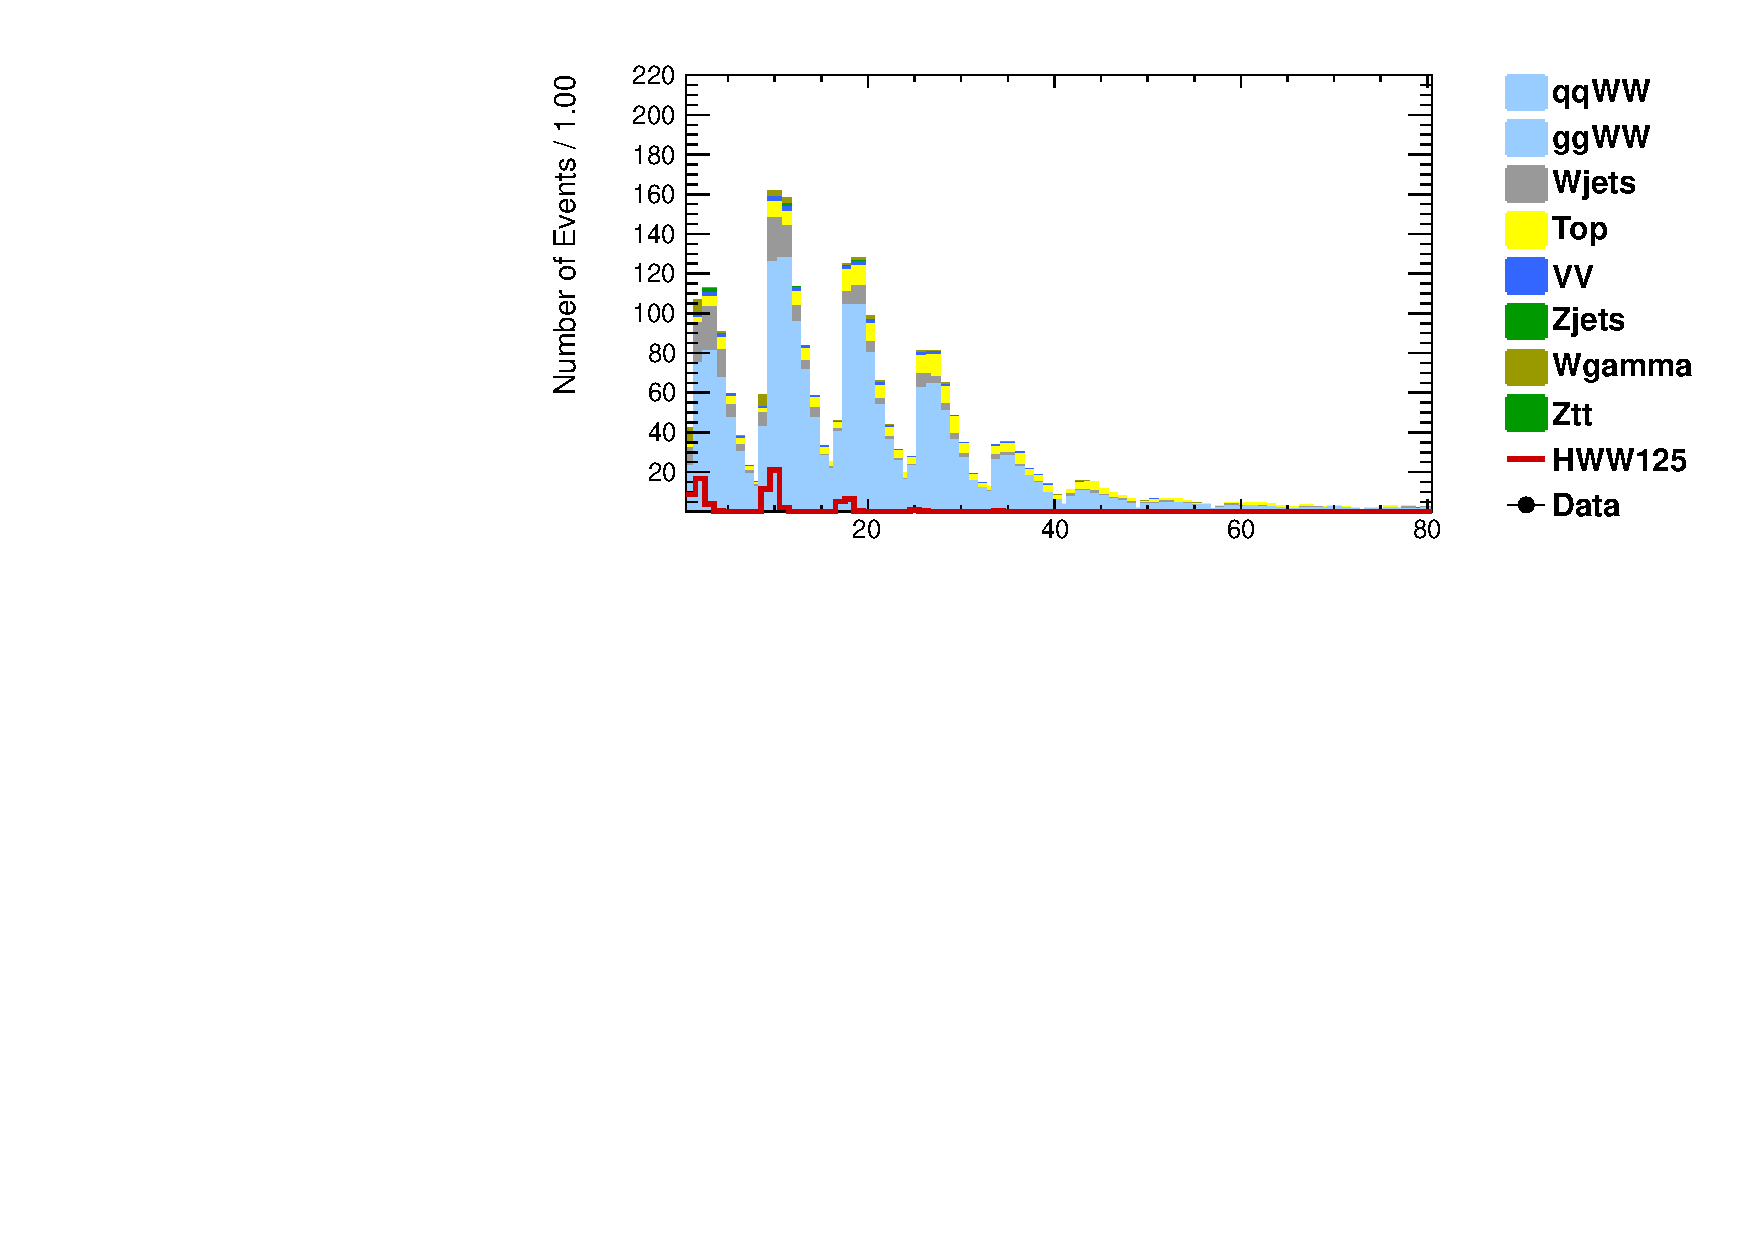
\includegraphics[width=.45\textwidth]{figures/templates/2D_mH125_0j_of_stack_lin.pdf}
	}
	\subfigure[Overlaid unrolled template linear]{
	\centering
	\label{subfig:template_unroll_overlay_lin}
		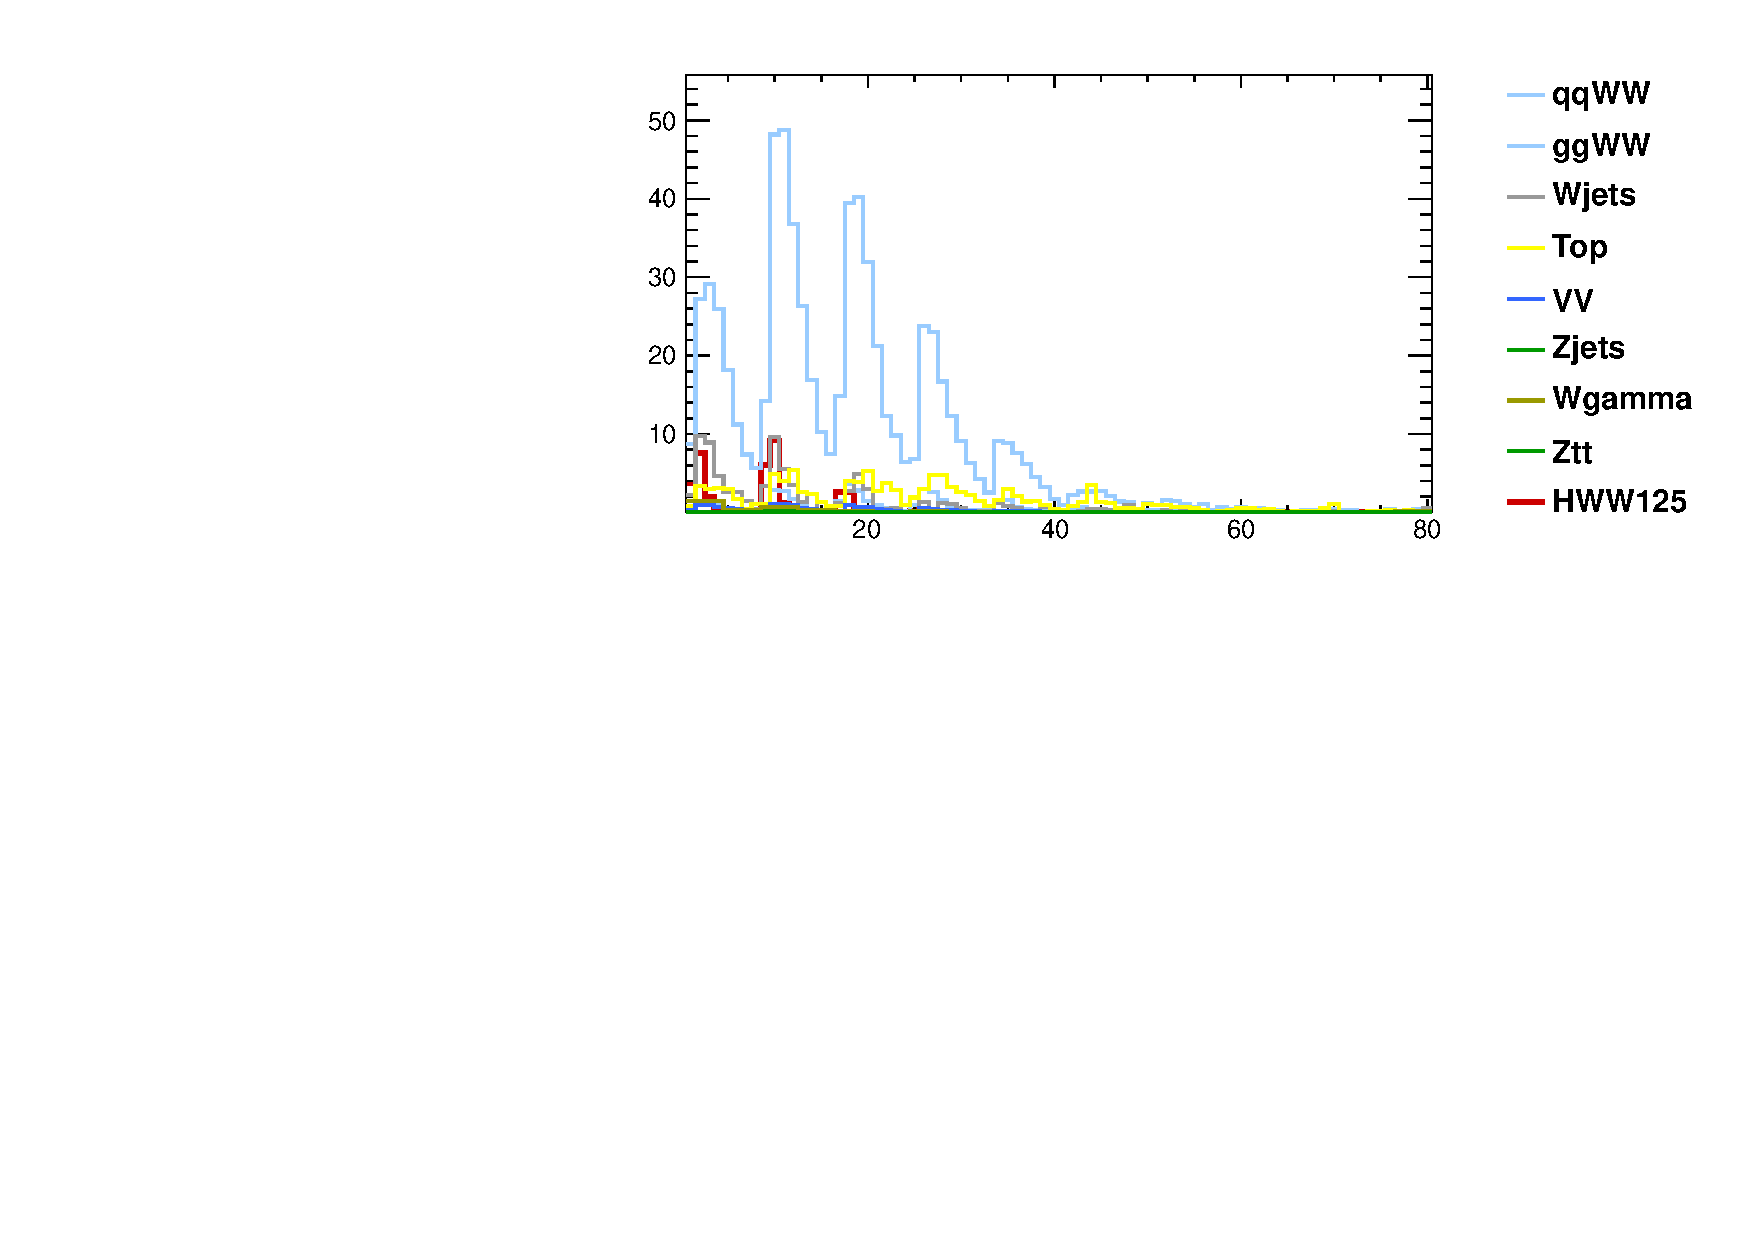
\includegraphics[width=.45\textwidth]{figures/templates/2D_mH125_0j_of_overlay_lin.pdf}
	}

	%
	\centering
	\subfigure[Stacked unrolled template in log scale]{
	\centering
	\label{subfig:template_unroll_stack_log}
		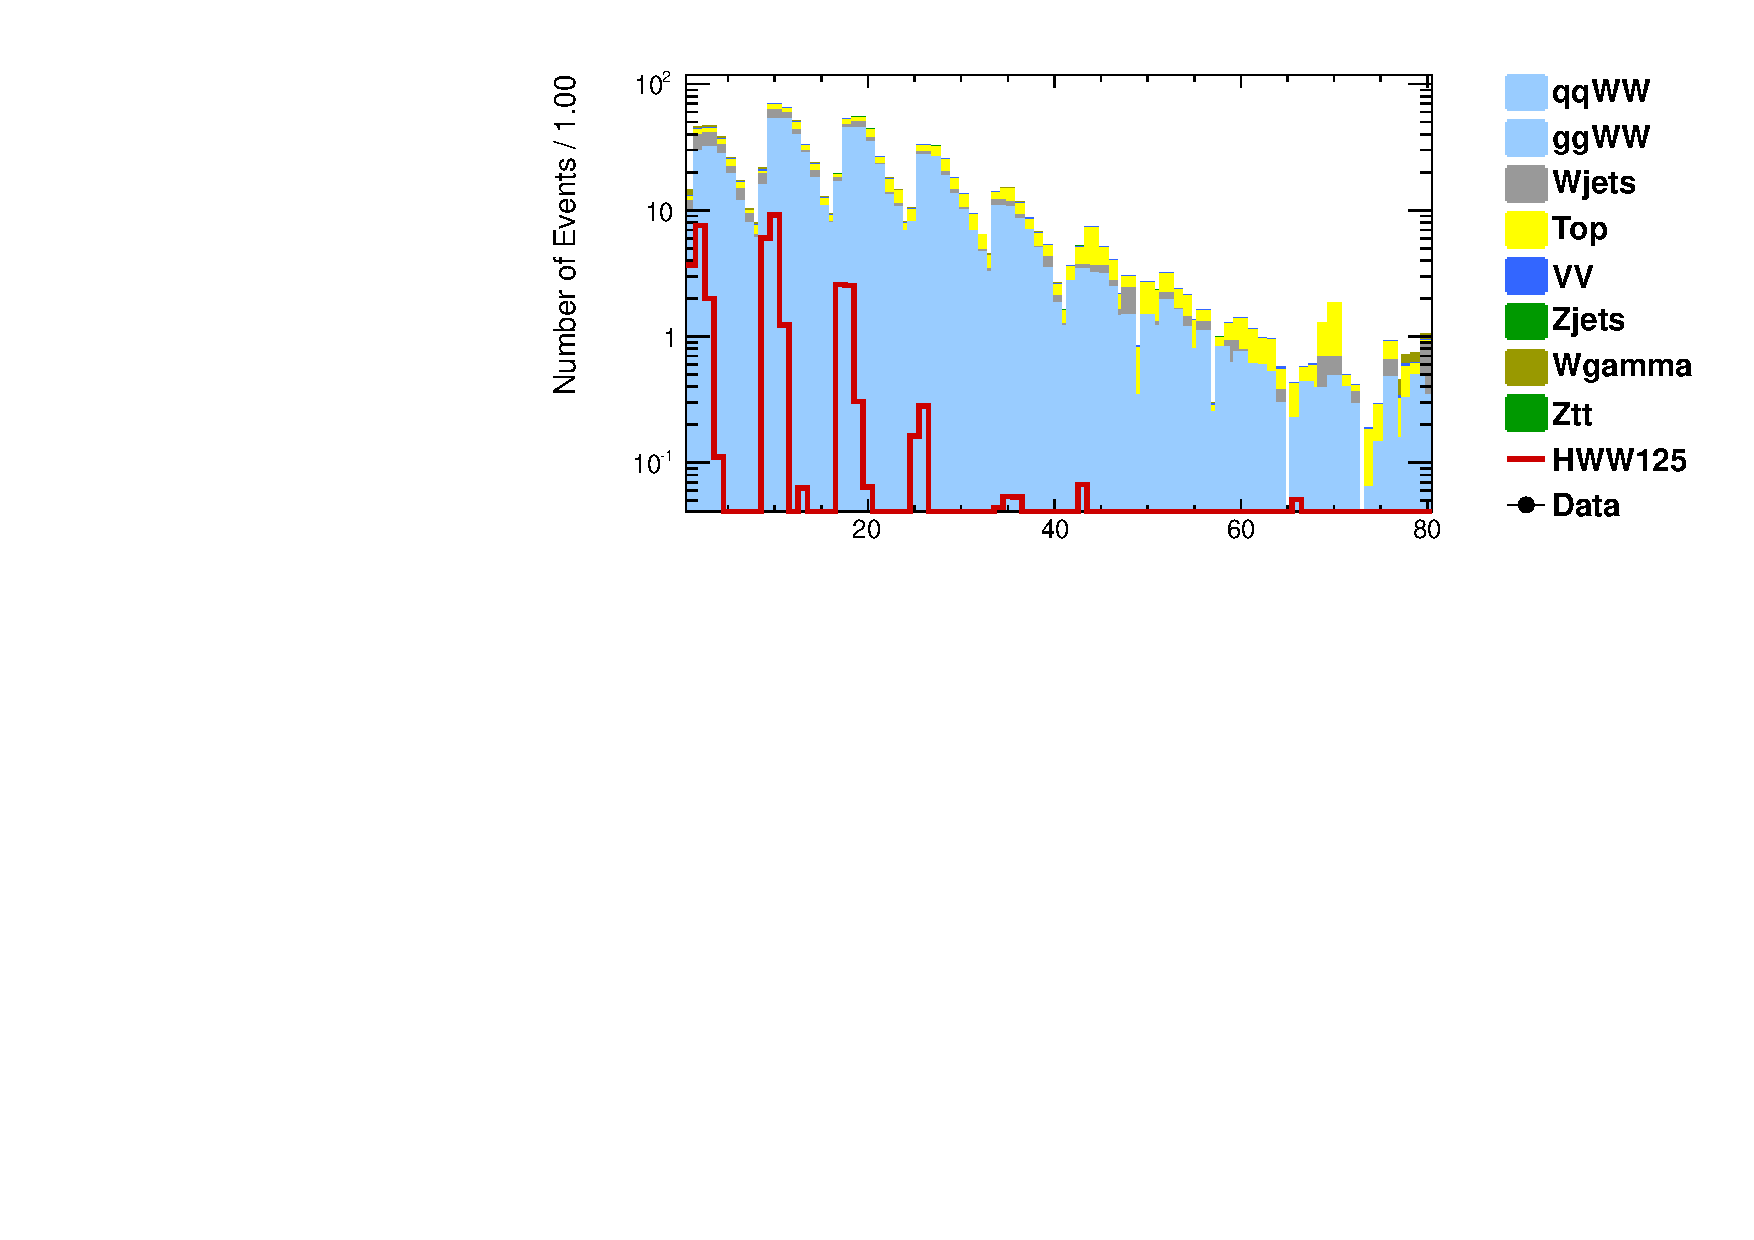
\includegraphics[width=.45\textwidth]{figures/templates/2D_mH125_0j_of_stack_log.pdf}
	}
	\subfigure[Overlaid unrolled template in log scale]{
	\centering
	\label{subfig:template_unroll_overlay_log}
		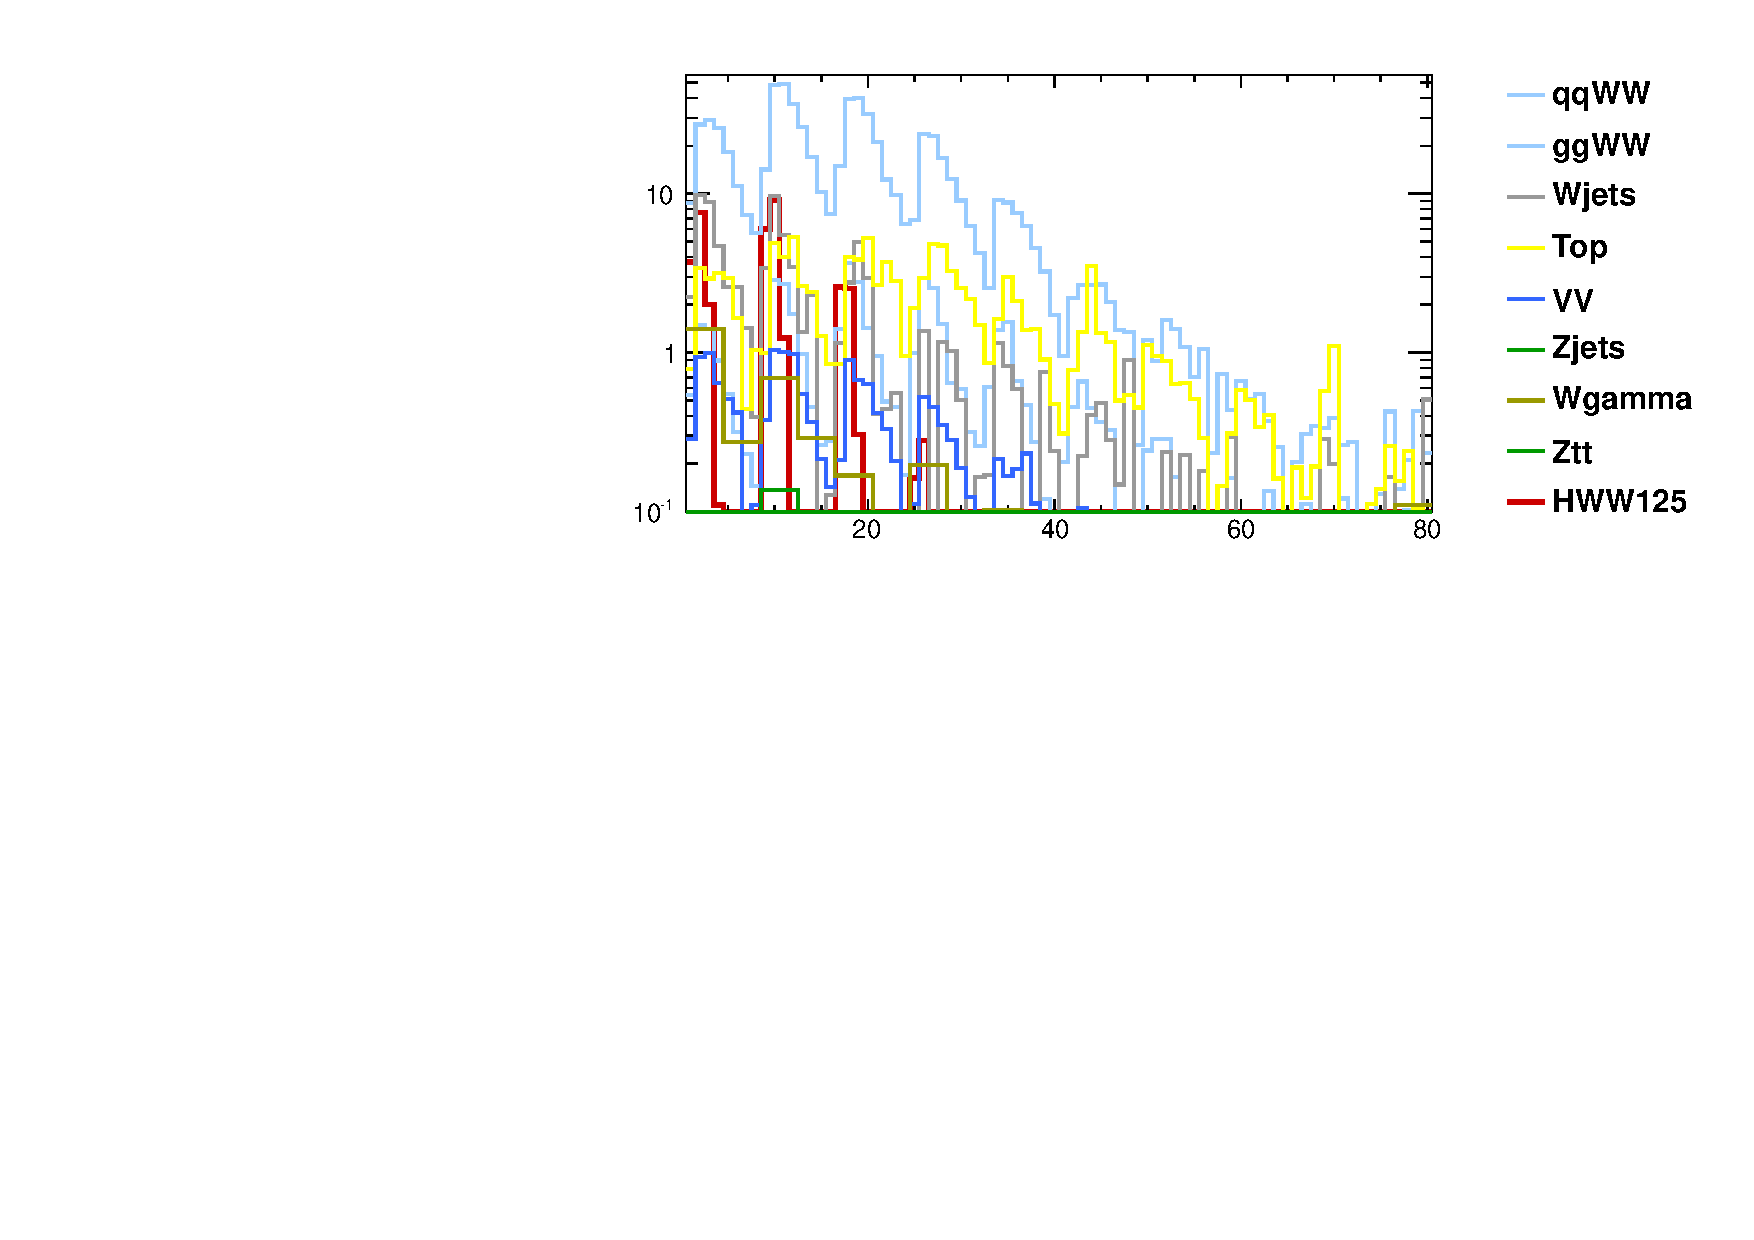
\includegraphics[width=.45\textwidth]{figures/templates/2D_mH125_0j_of_overlay_log.pdf}
	}

	\caption{Unrolled templates at \mHi = 125 \GeV in 0jet bin.} 
	\label{fig:templates_125_0j_unroll}

\end{figure} 

\newpage
%%% mH=600 0jet
\begin{figure}[!hbtp]
	
	%
	\centering
	\subfigure[Signal]{
	\centering
	\label{subfig:template_signal_600}
		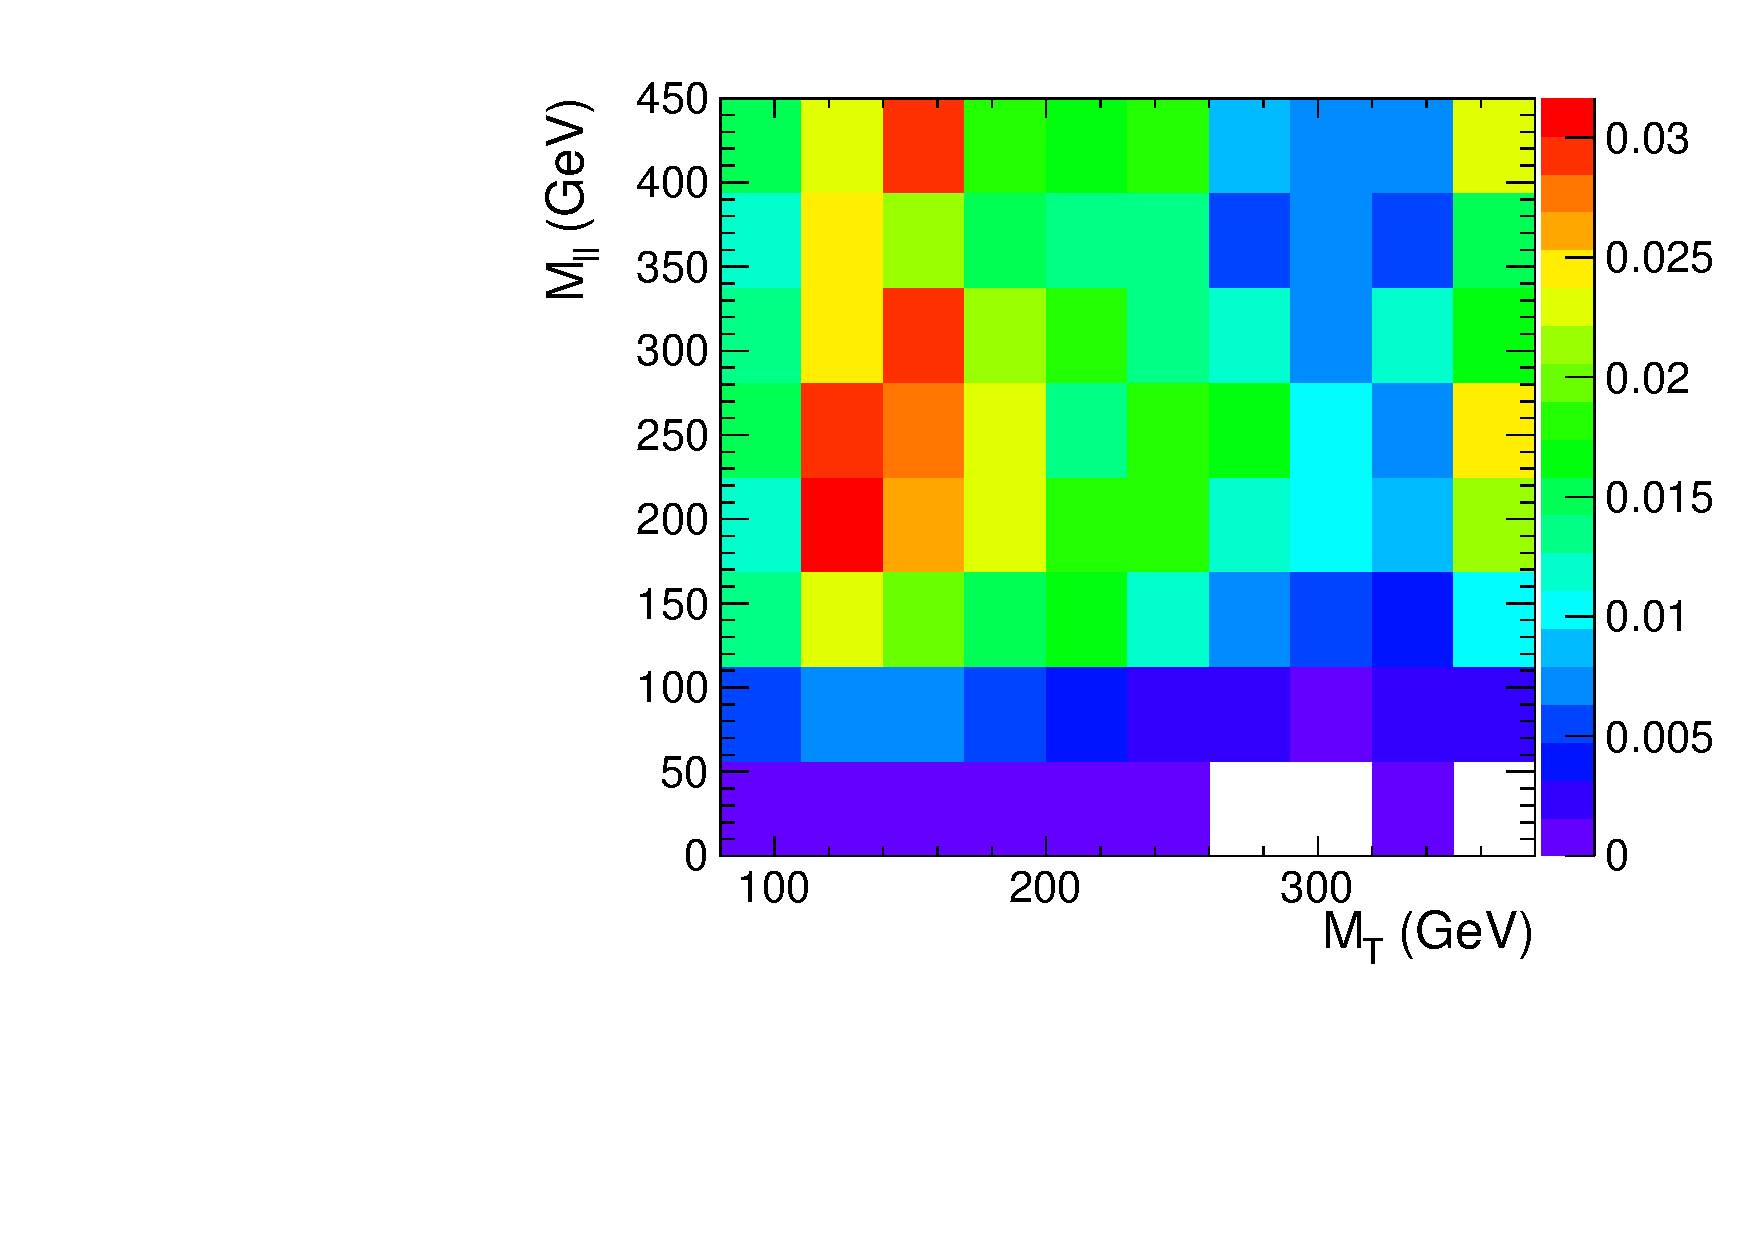
\includegraphics[width=.35\textwidth]{figures/templates/sig_2D_mH600_0j_of.pdf}
	}
	\subfigure[Signal statistical uncertainty]{
	\centering
	\label{subfig:template_signalerr_600}
		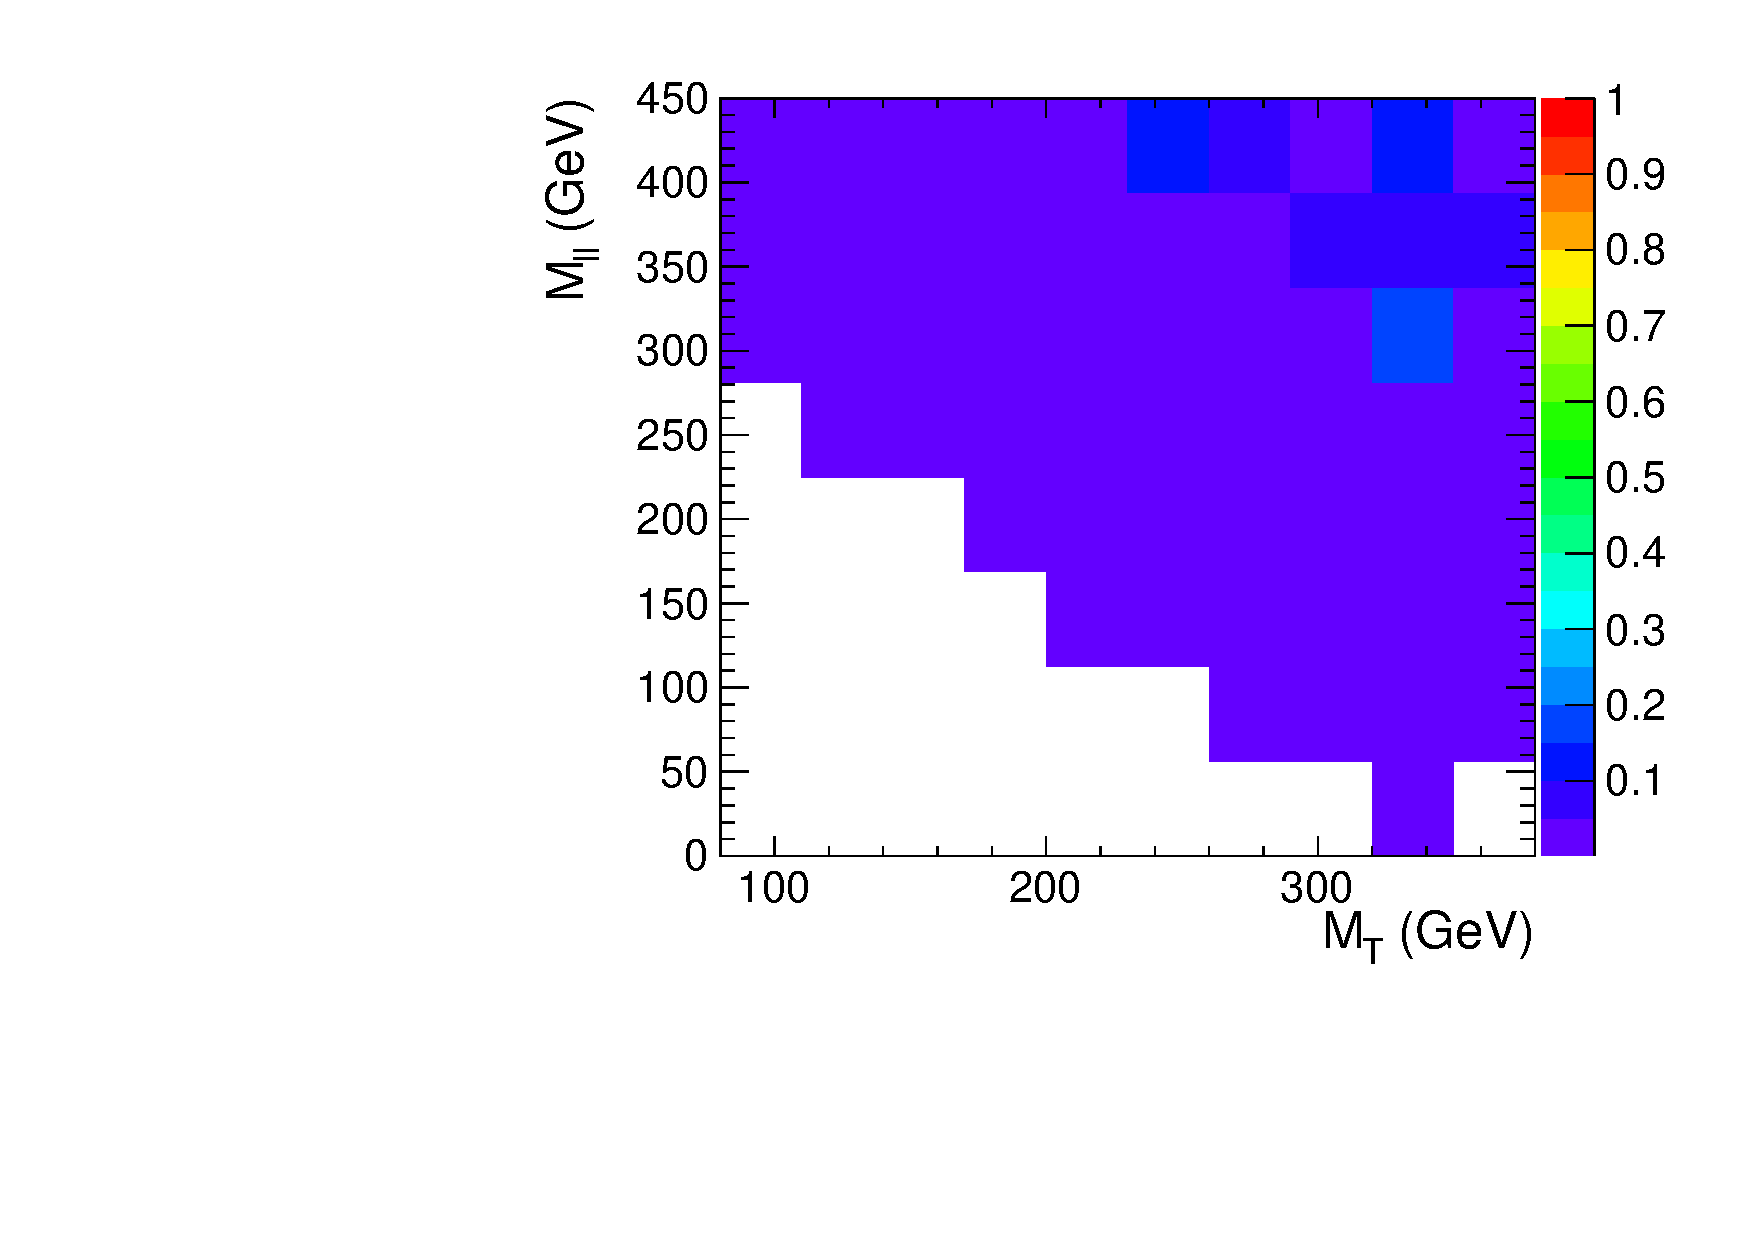
\includegraphics[width=.35\textwidth]{figures/templates/sigerr_2D_mH600_0j_of.pdf}
	}
	
	%
	\centering
	\subfigure[qqWW]{
	\centering
	\label{subfig:template_qqWW_600}
		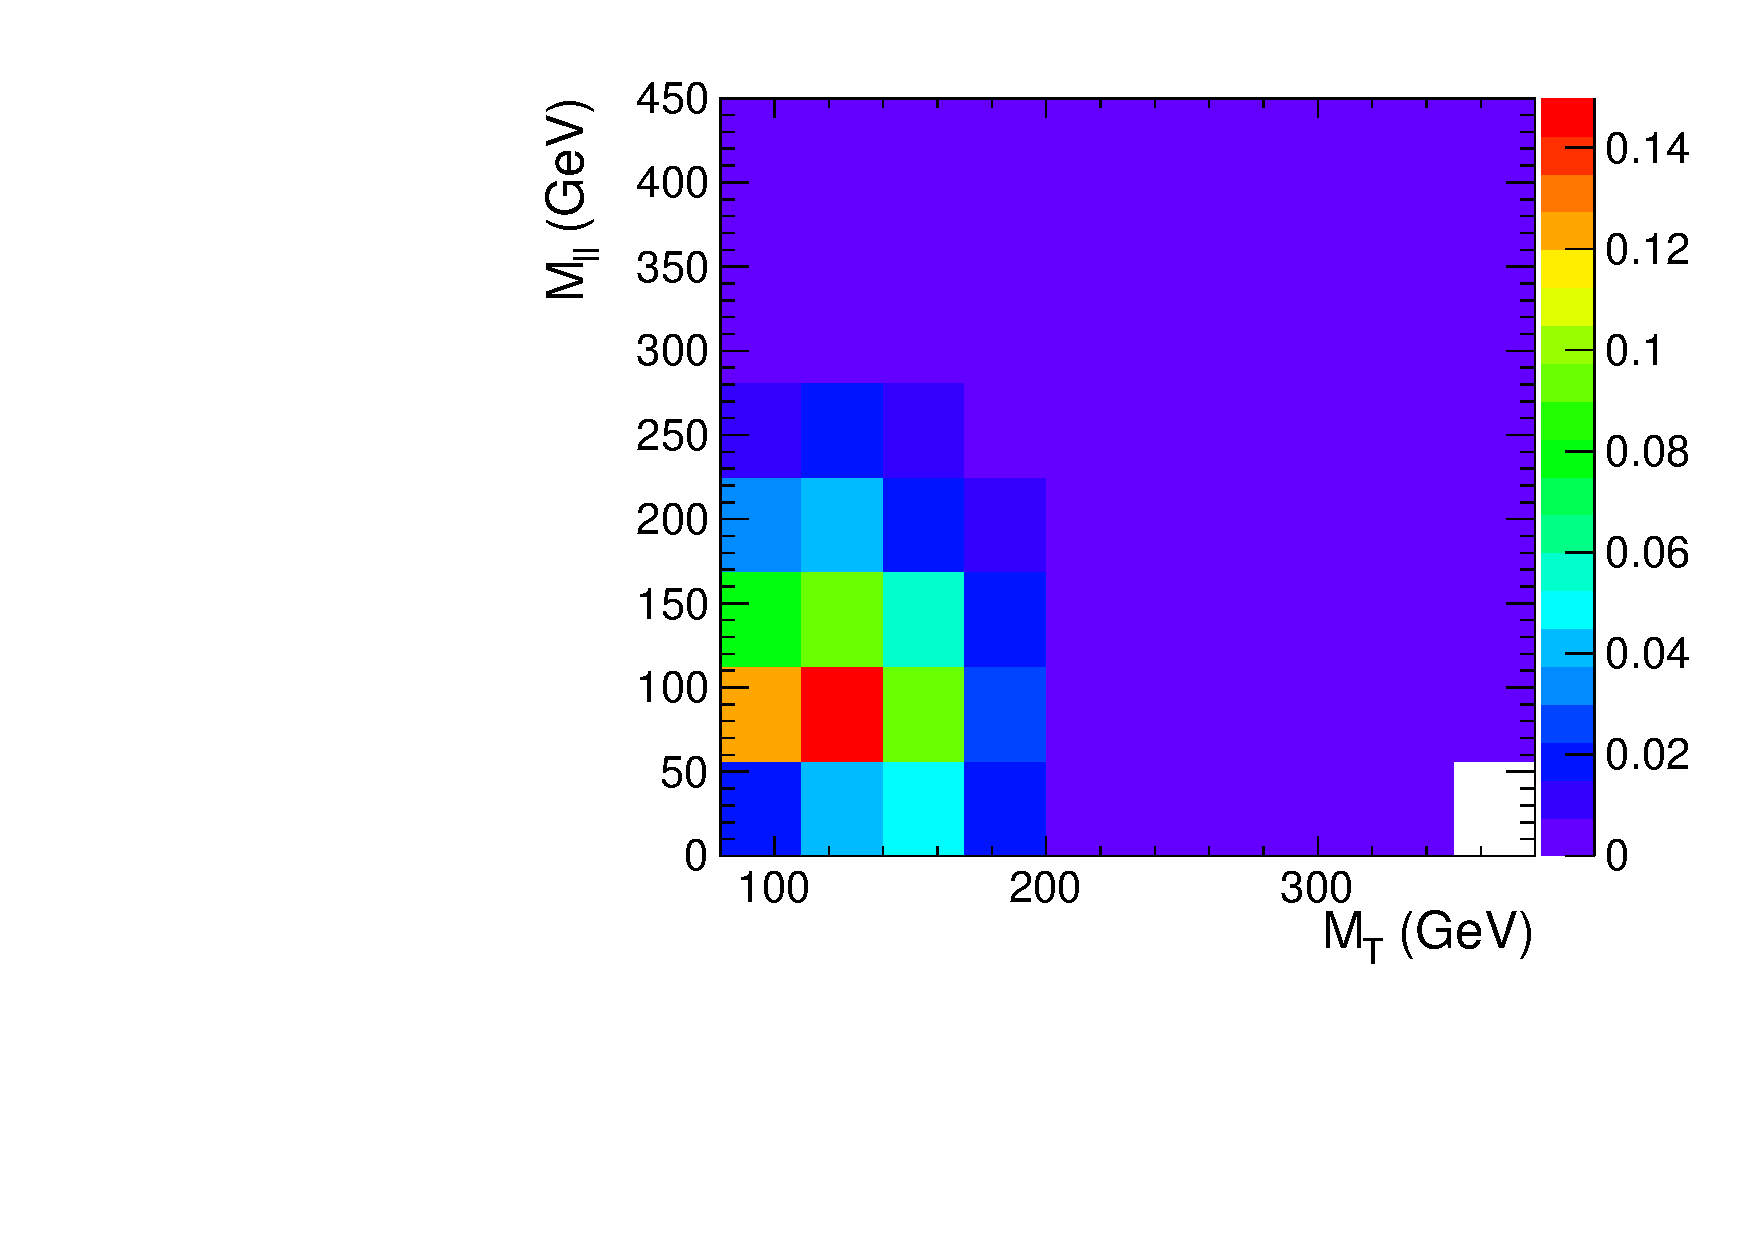
\includegraphics[width=.35\textwidth]{figures/templates/qqWW_2D_mH600_0j_of.pdf}
	}
	\subfigure[qqWW statistical uncertainty]{
	\centering
	\label{subfig:template_qqWWerr_600}
		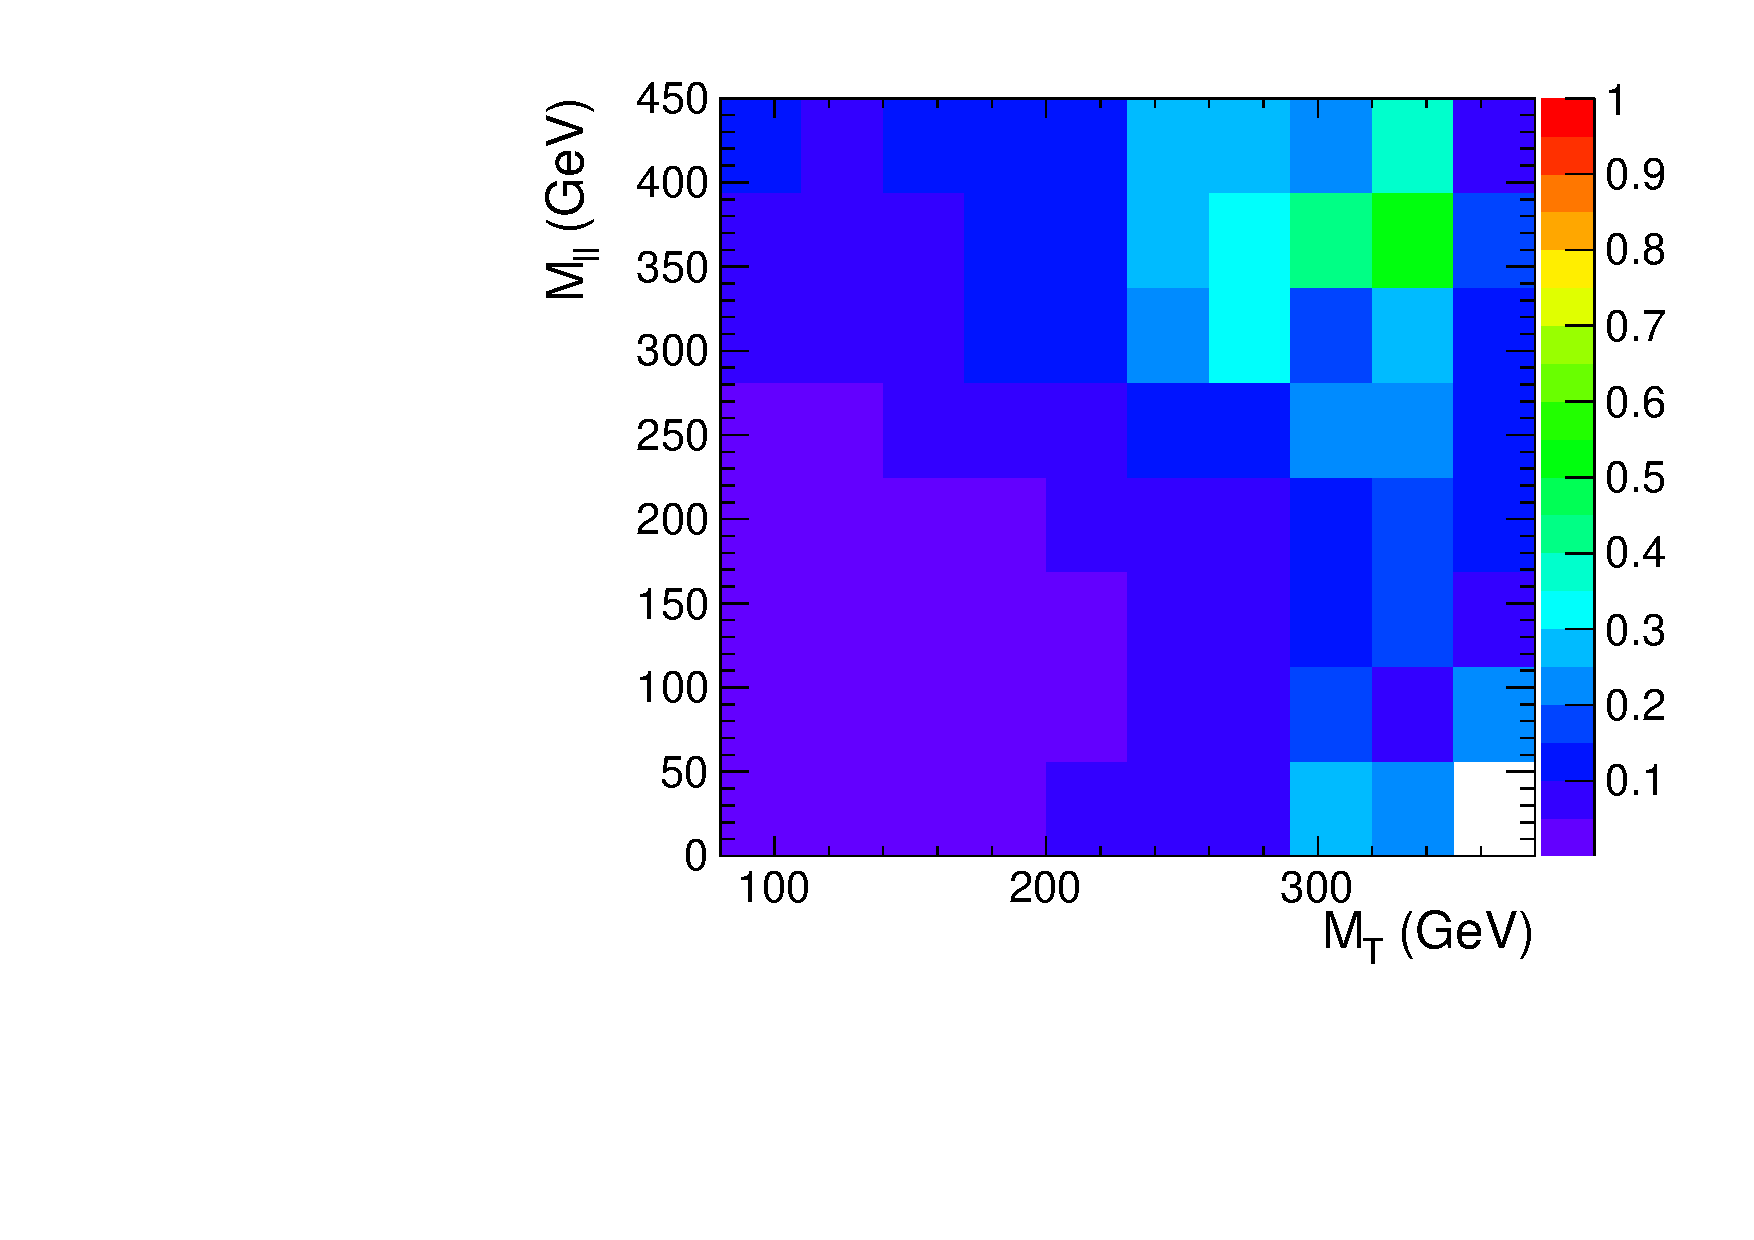
\includegraphics[width=.35\textwidth]{figures/templates/qqWWerr_2D_mH600_0j_of.pdf}
	}

	%
	\centering
	\subfigure[ggWW]{
	\centering
	\label{subfig:template_ggWW_600}
		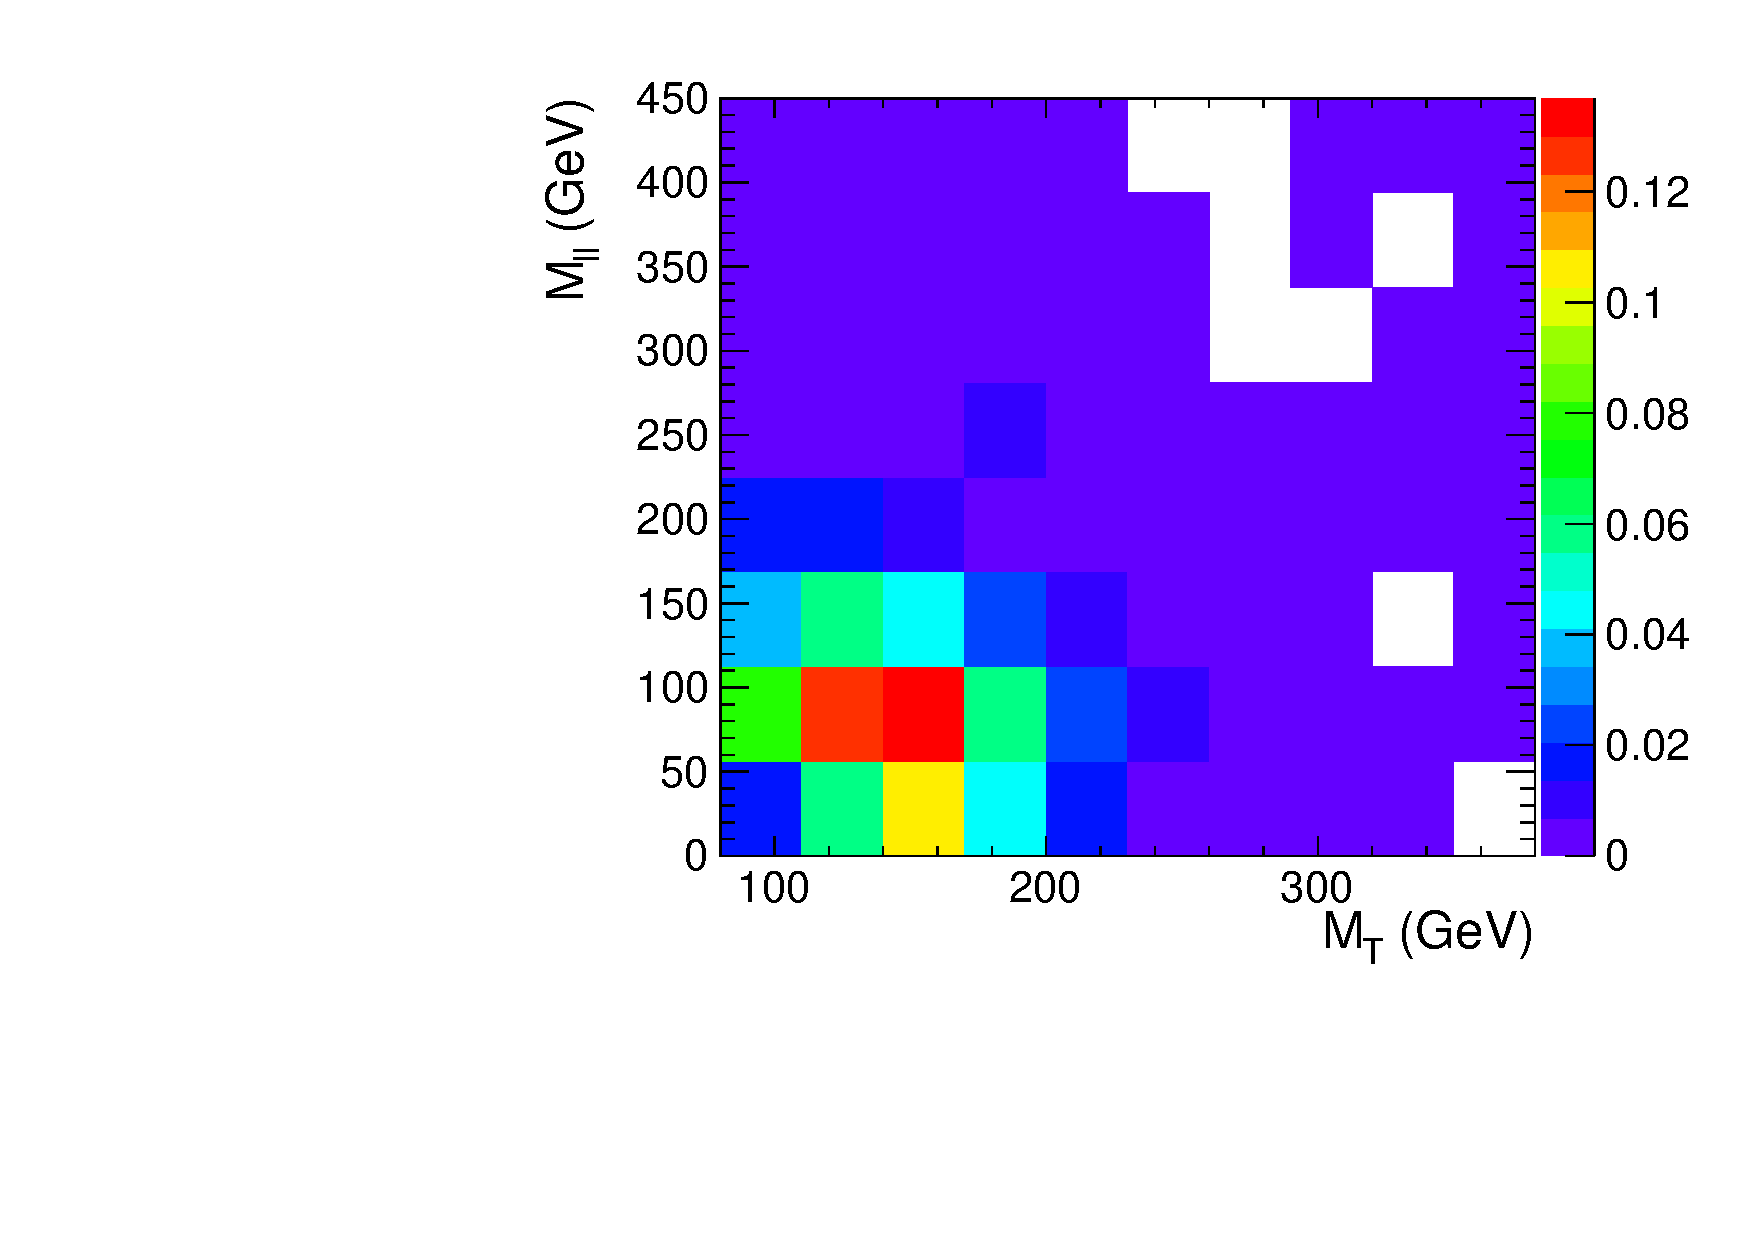
\includegraphics[width=.35\textwidth]{figures/templates/ggWW_2D_mH600_0j_of.pdf}
	}
	\subfigure[ggWW statistical uncertainty]{
	\centering
	\label{subfig:template_ggWWerr_600}
		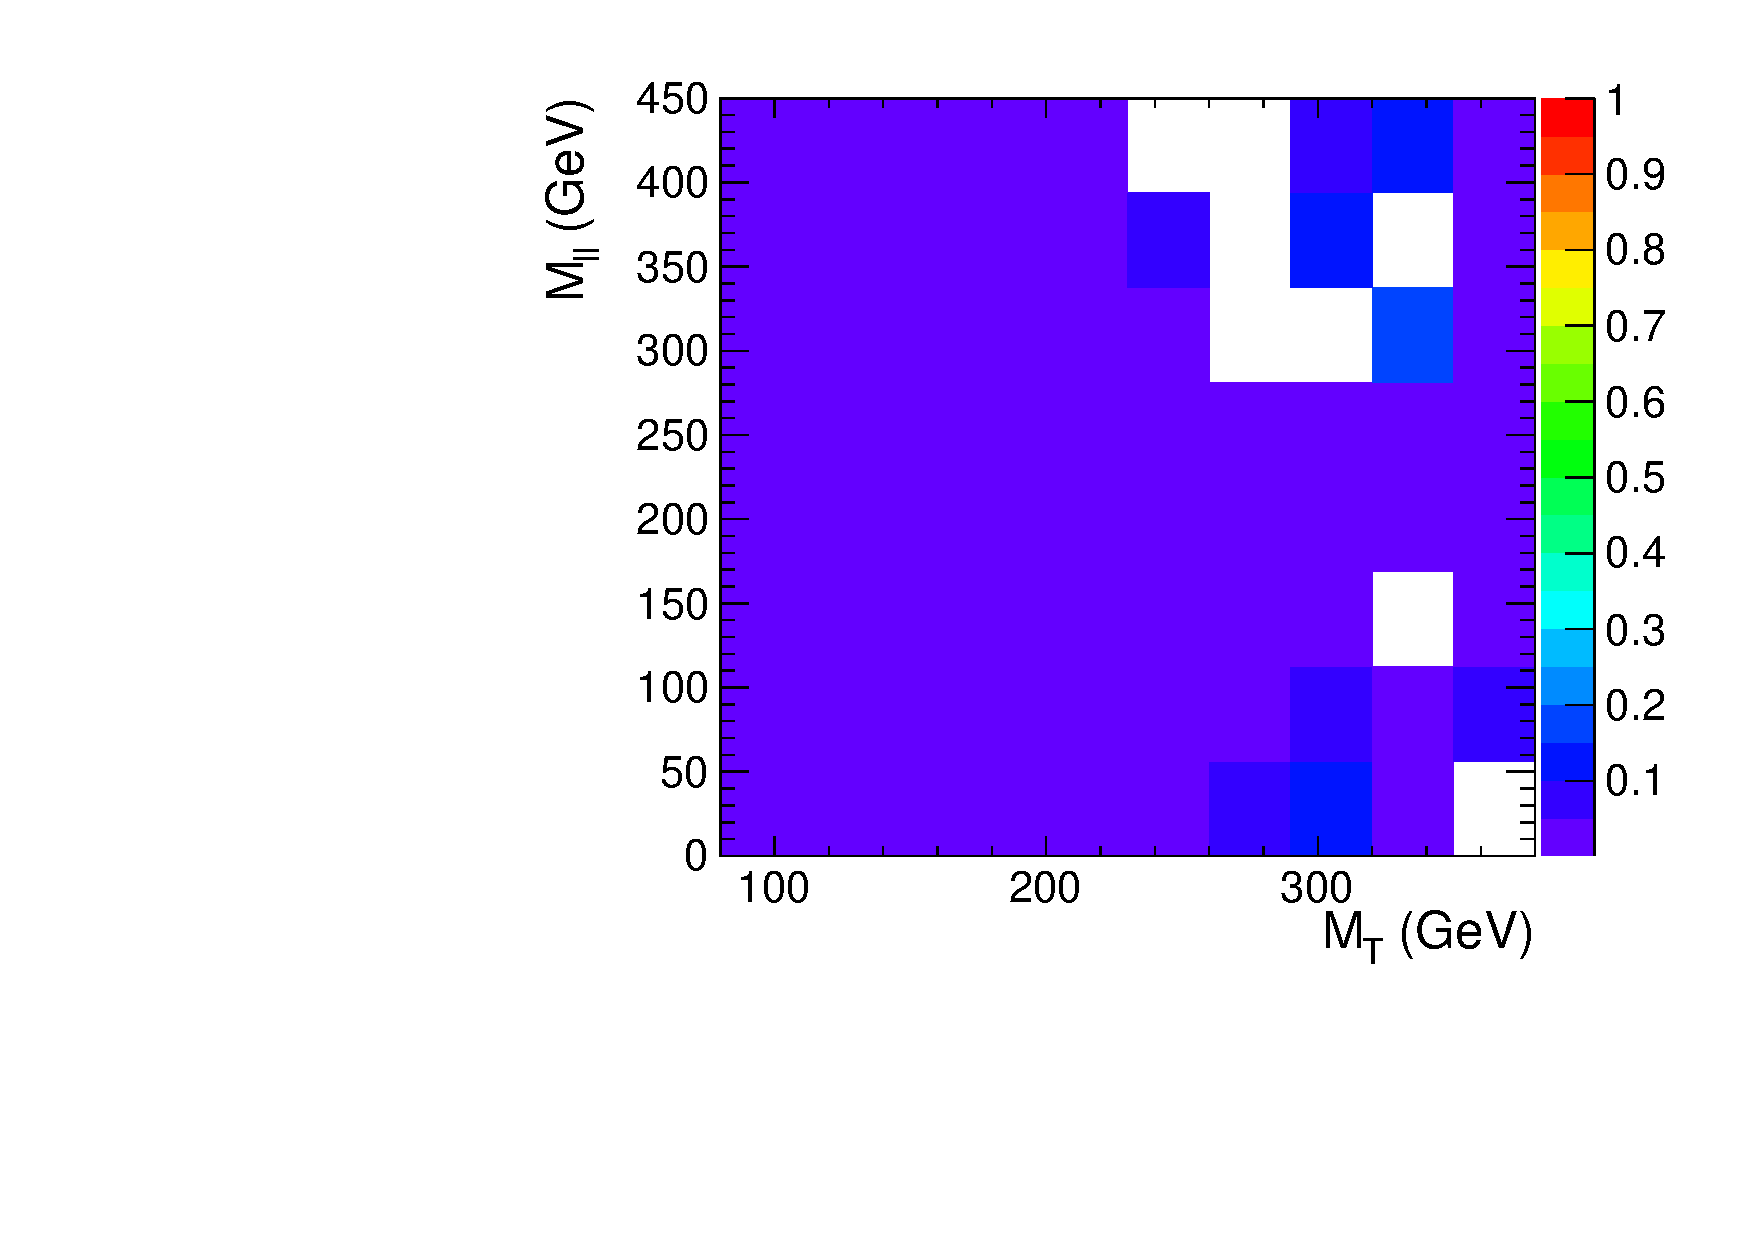
\includegraphics[width=.35\textwidth]{figures/templates/ggWWerr_2D_mH600_0j_of.pdf}
	}

	\caption{2D templates at \mHi = 600 \GeV in 0 jet bin} 
	\label{fig:templates_600_0j_1}

\end{figure}

\begin{figure}[!hbtp]
	
	%
	\centering
	\subfigure[Wjets]{
	\centering
	\label{subfig:template_Wjets_600}
		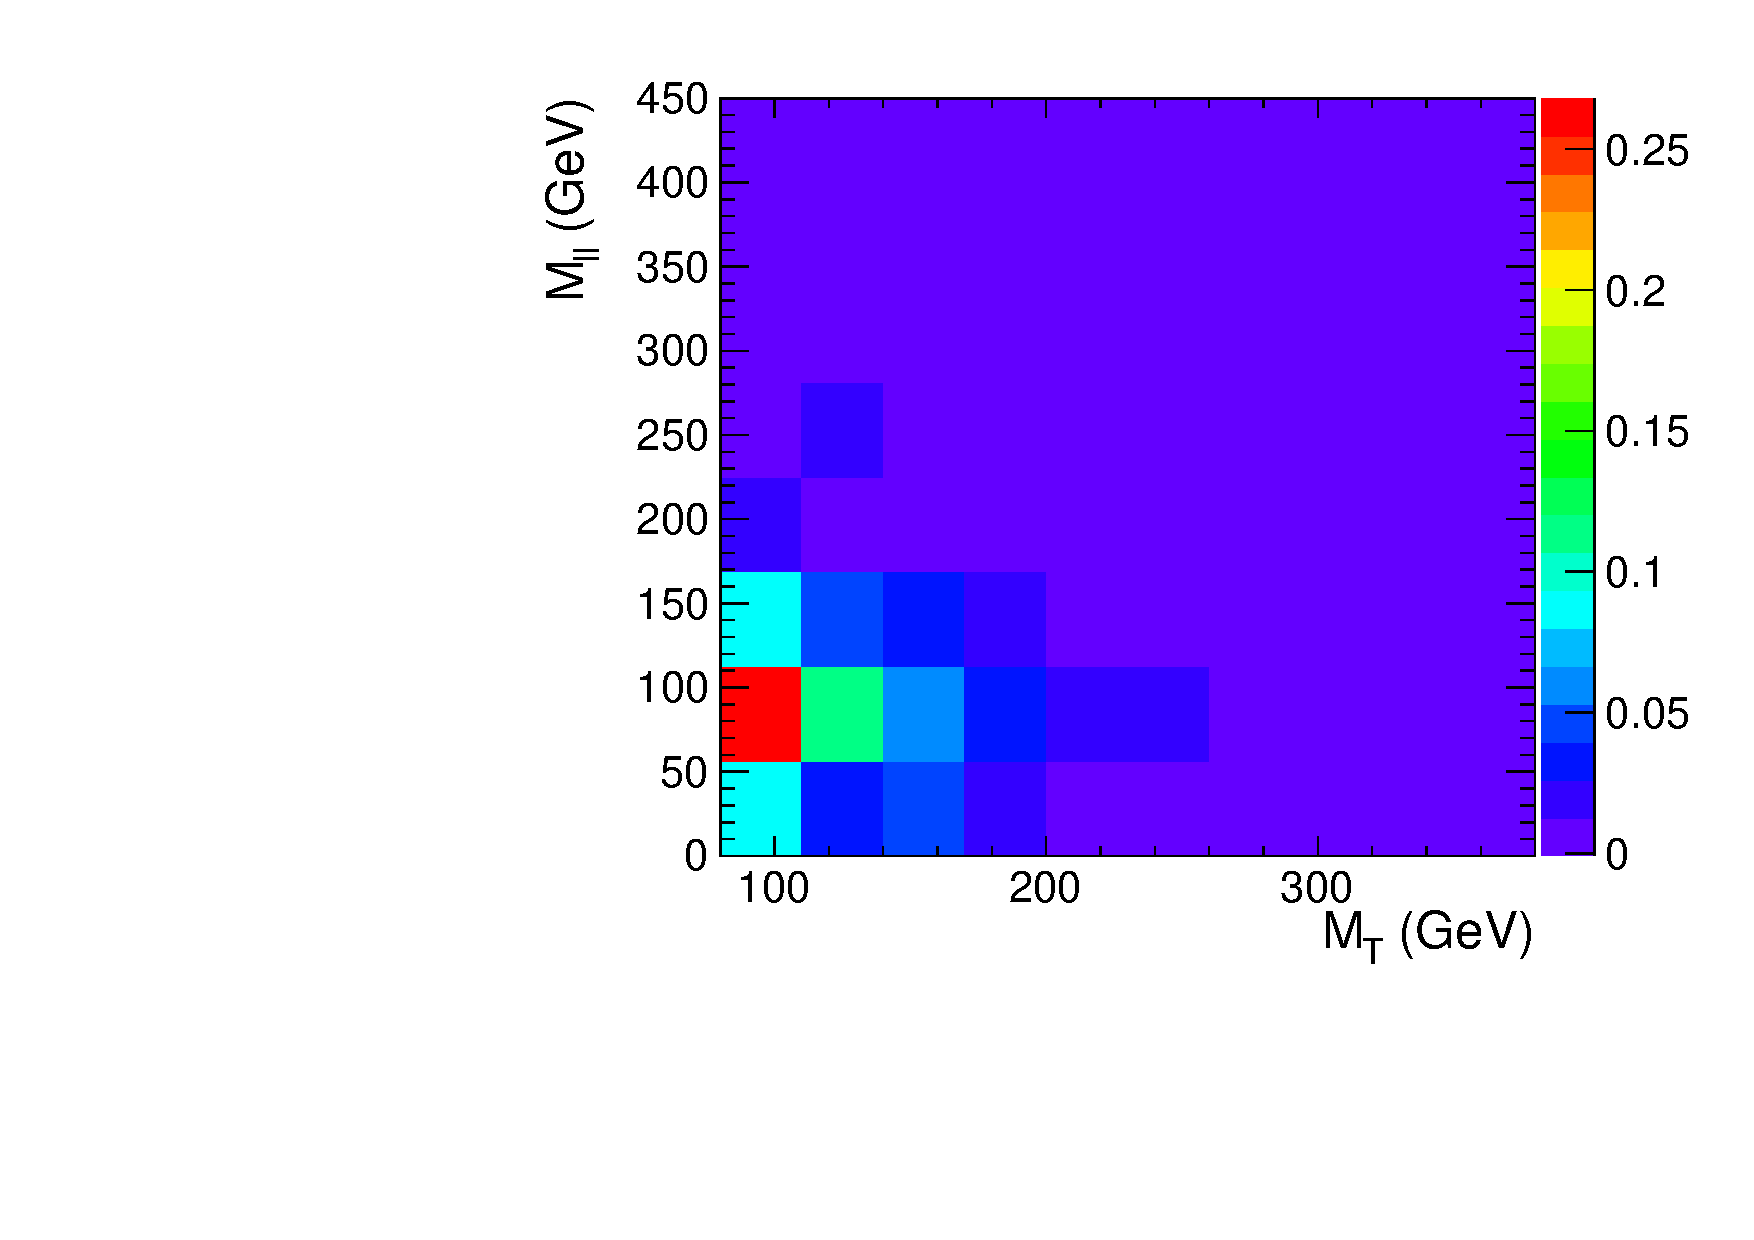
\includegraphics[width=.35\textwidth]{figures/templates/Wjets_2D_mH600_0j_of.pdf}
	}
	\subfigure[Wjets statistical uncertainty]{
	\centering
	\label{subfig:template_Wjetserr_600}
		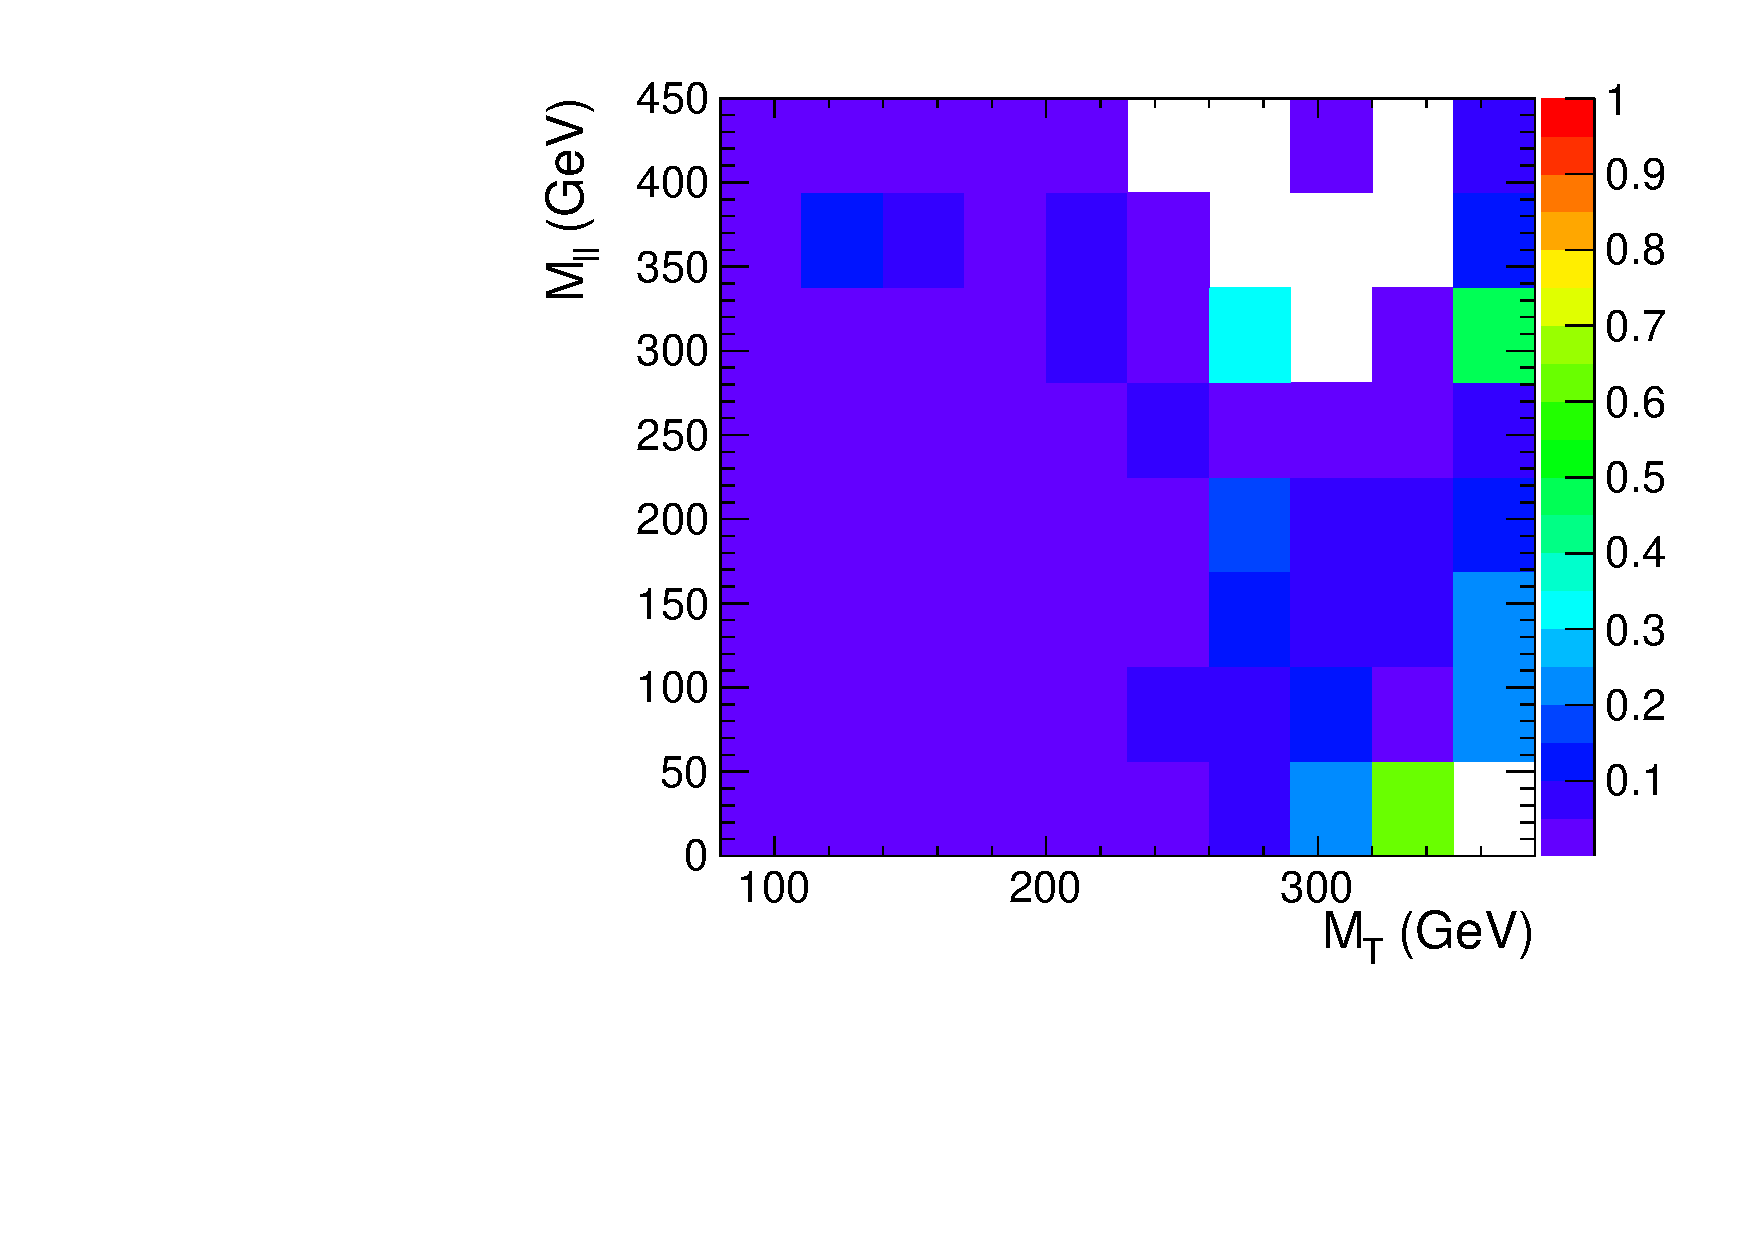
\includegraphics[width=.35\textwidth]{figures/templates/Wjetserr_2D_mH600_0j_of.pdf}
	}
	
	%
	\centering
	\subfigure[Top]{
	\centering
	\label{subfig:template_Top_600}
		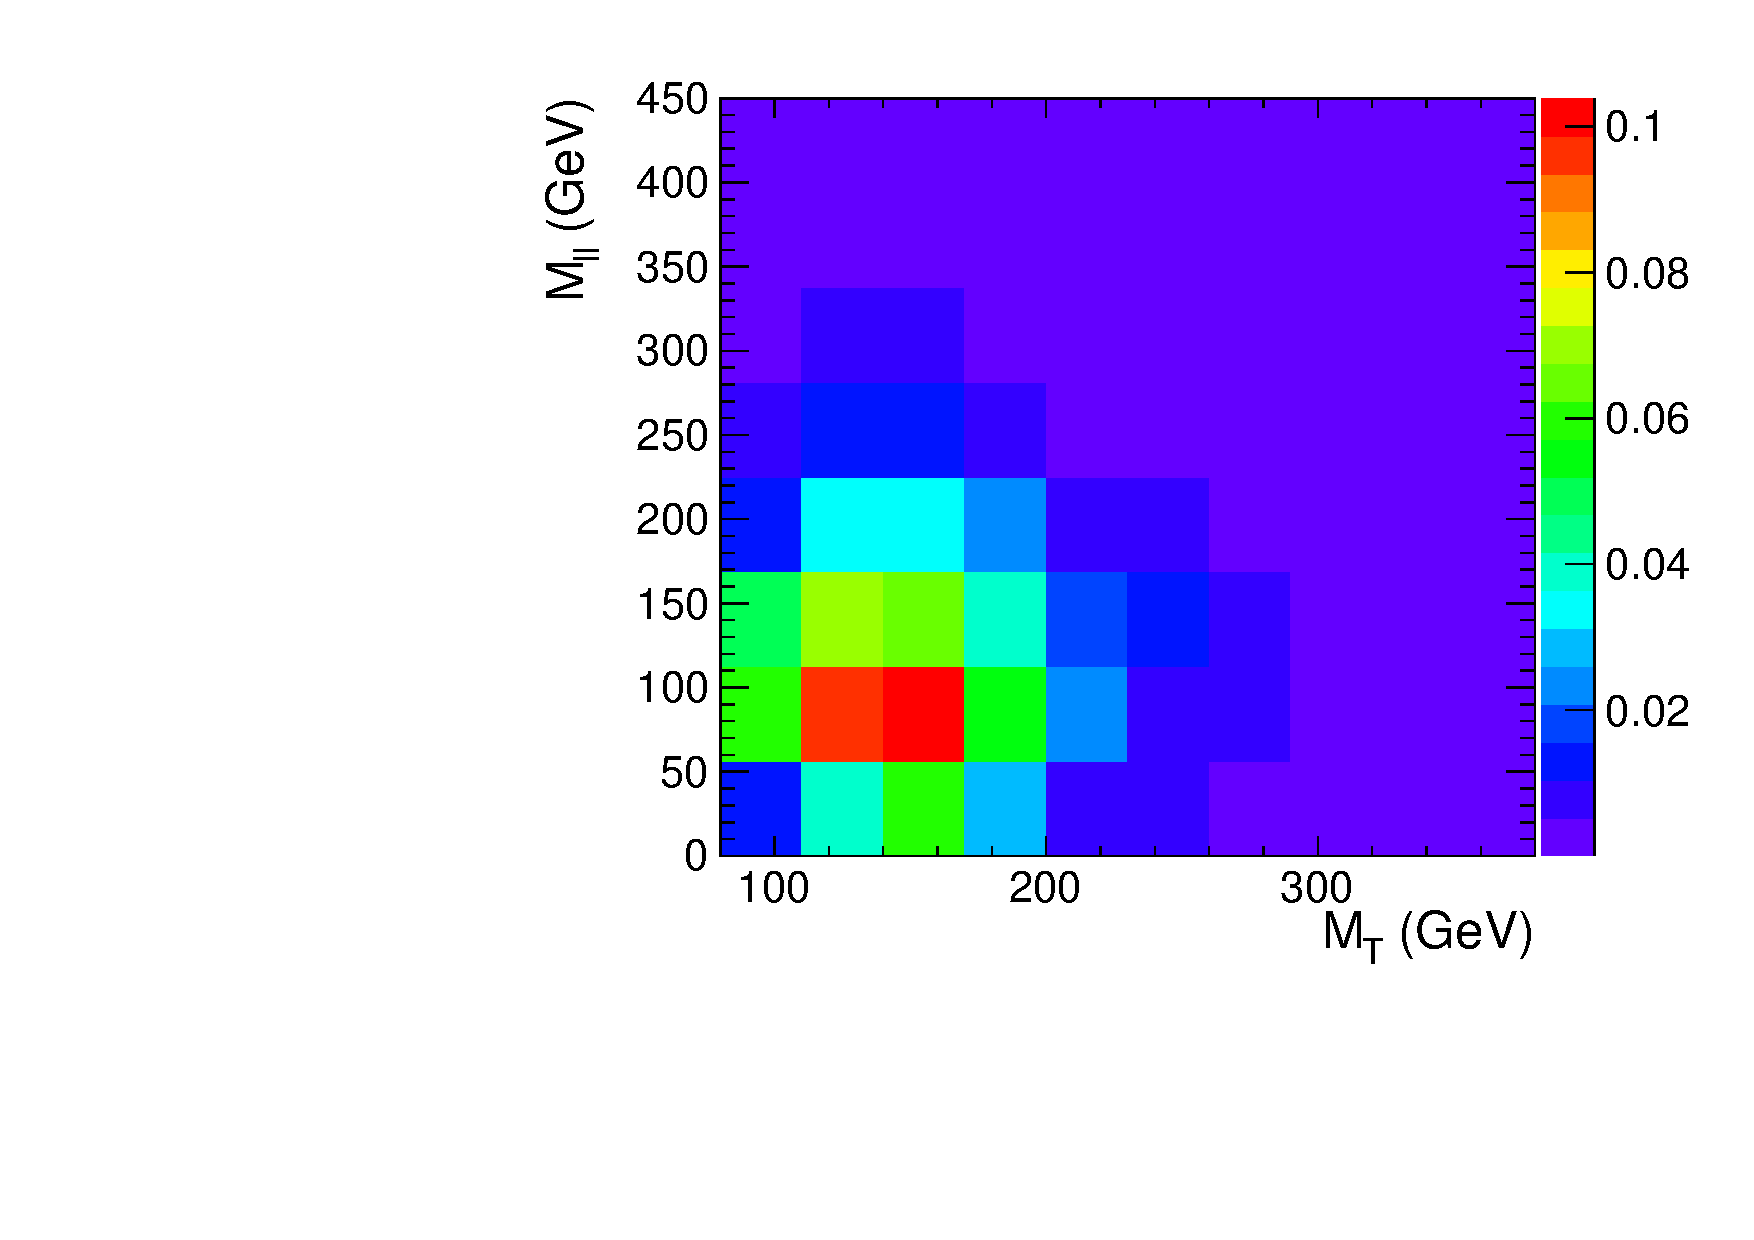
\includegraphics[width=.35\textwidth]{figures/templates/Top_2D_mH600_0j_of.pdf}
	}
	\subfigure[Top statistical uncertainty]{
	\centering
	\label{subfig:template_Toperr_600}
		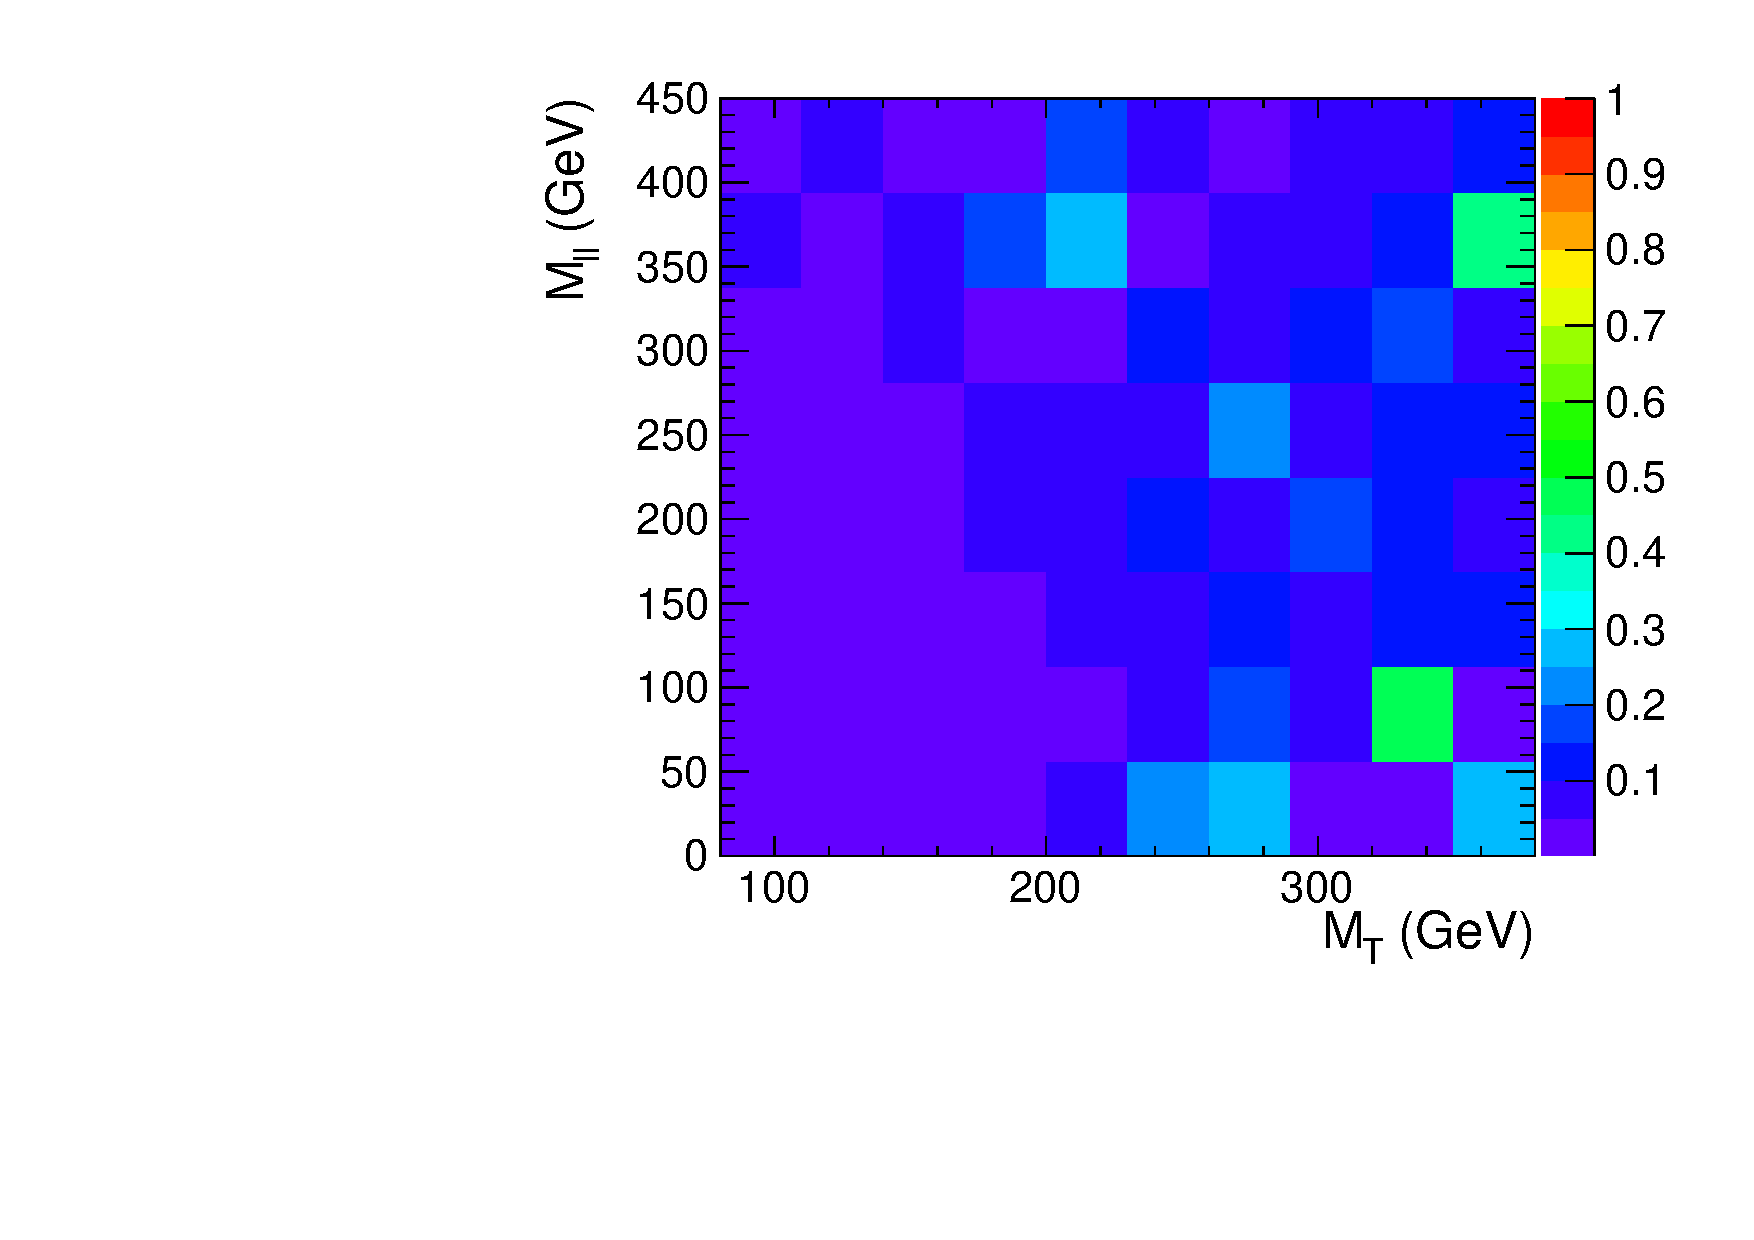
\includegraphics[width=.35\textwidth]{figures/templates/Toperr_2D_mH600_0j_of.pdf}
	}

	%
	\centering
	\subfigure[VV]{
	\centering
	\label{subfig:template_VV_600}
		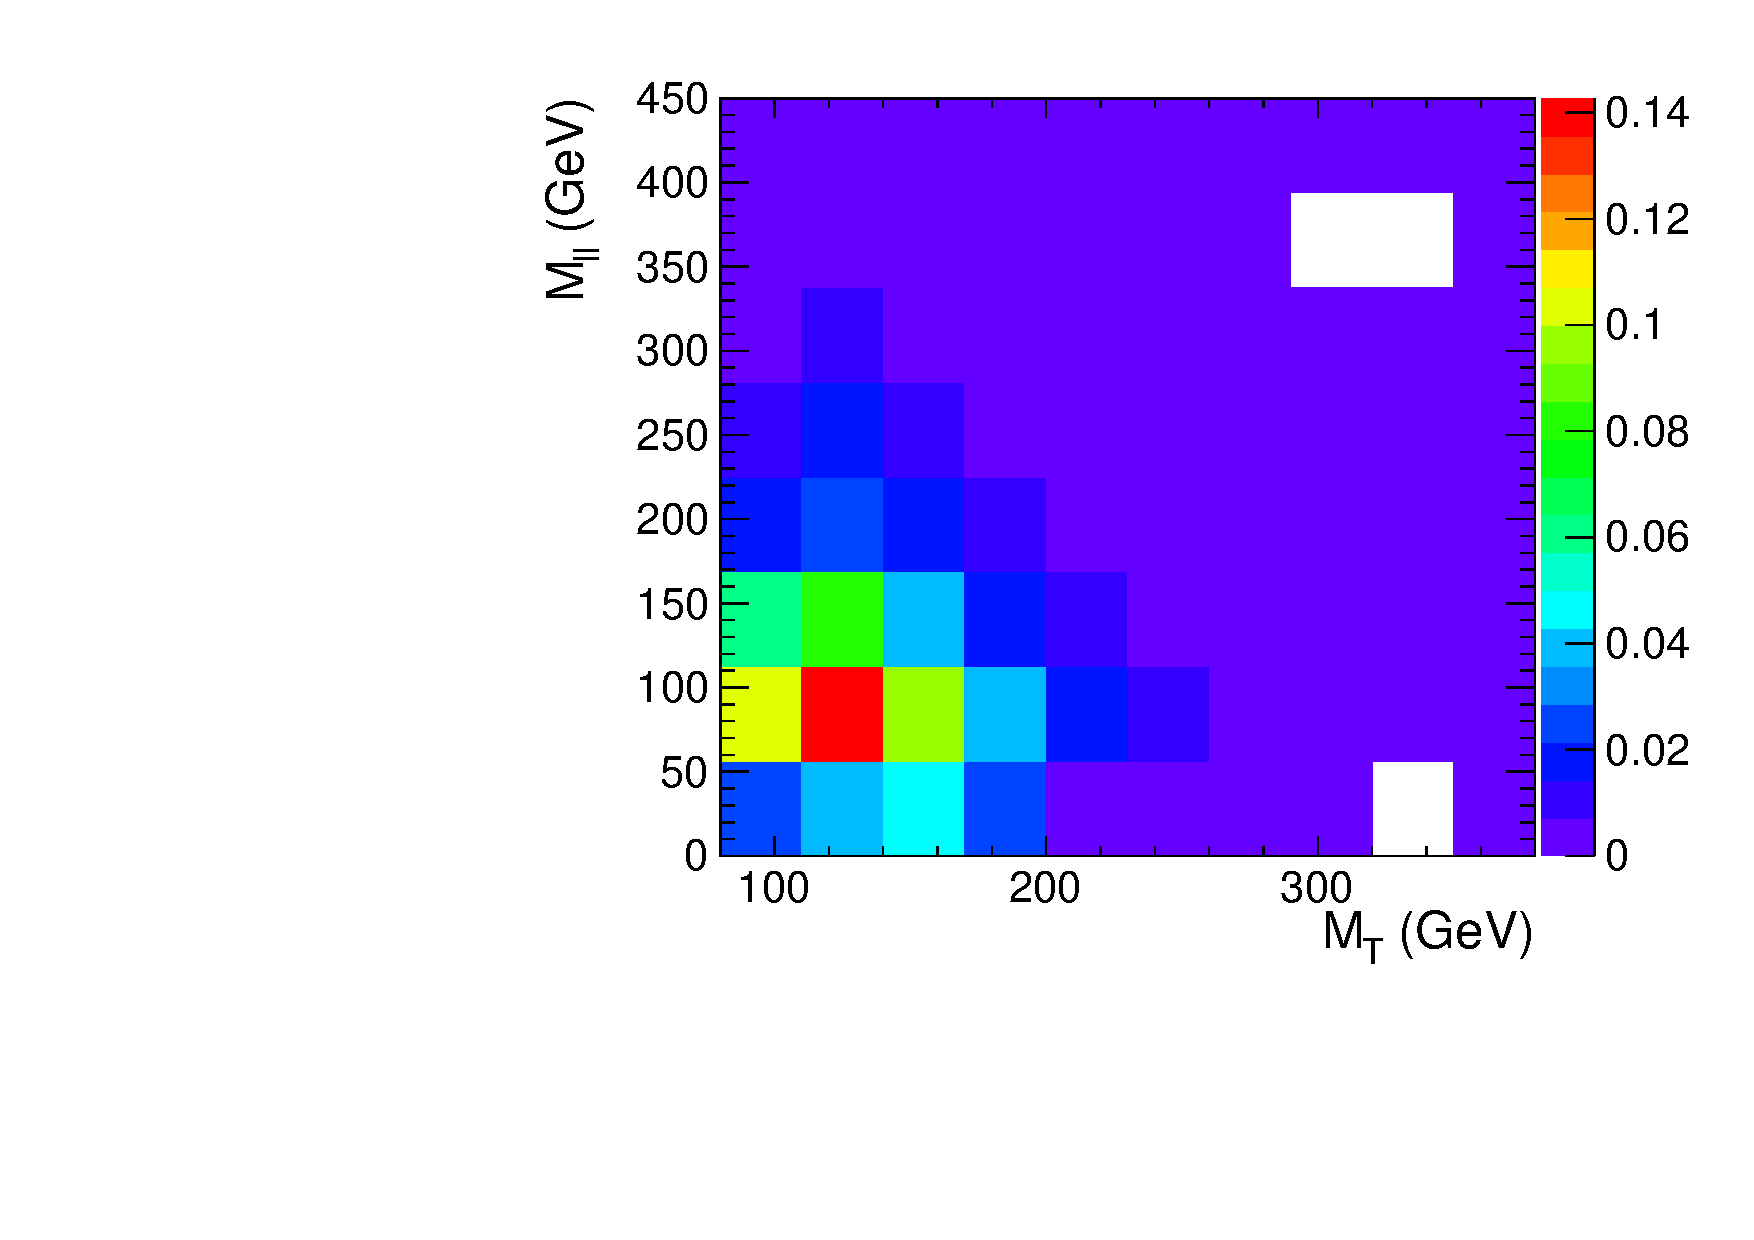
\includegraphics[width=.35\textwidth]{figures/templates/VV_2D_mH600_0j_of.pdf}
	}
	\subfigure[VV statistical uncertainty]{
	\centering
	\label{subfig:template_VVerr_600}
		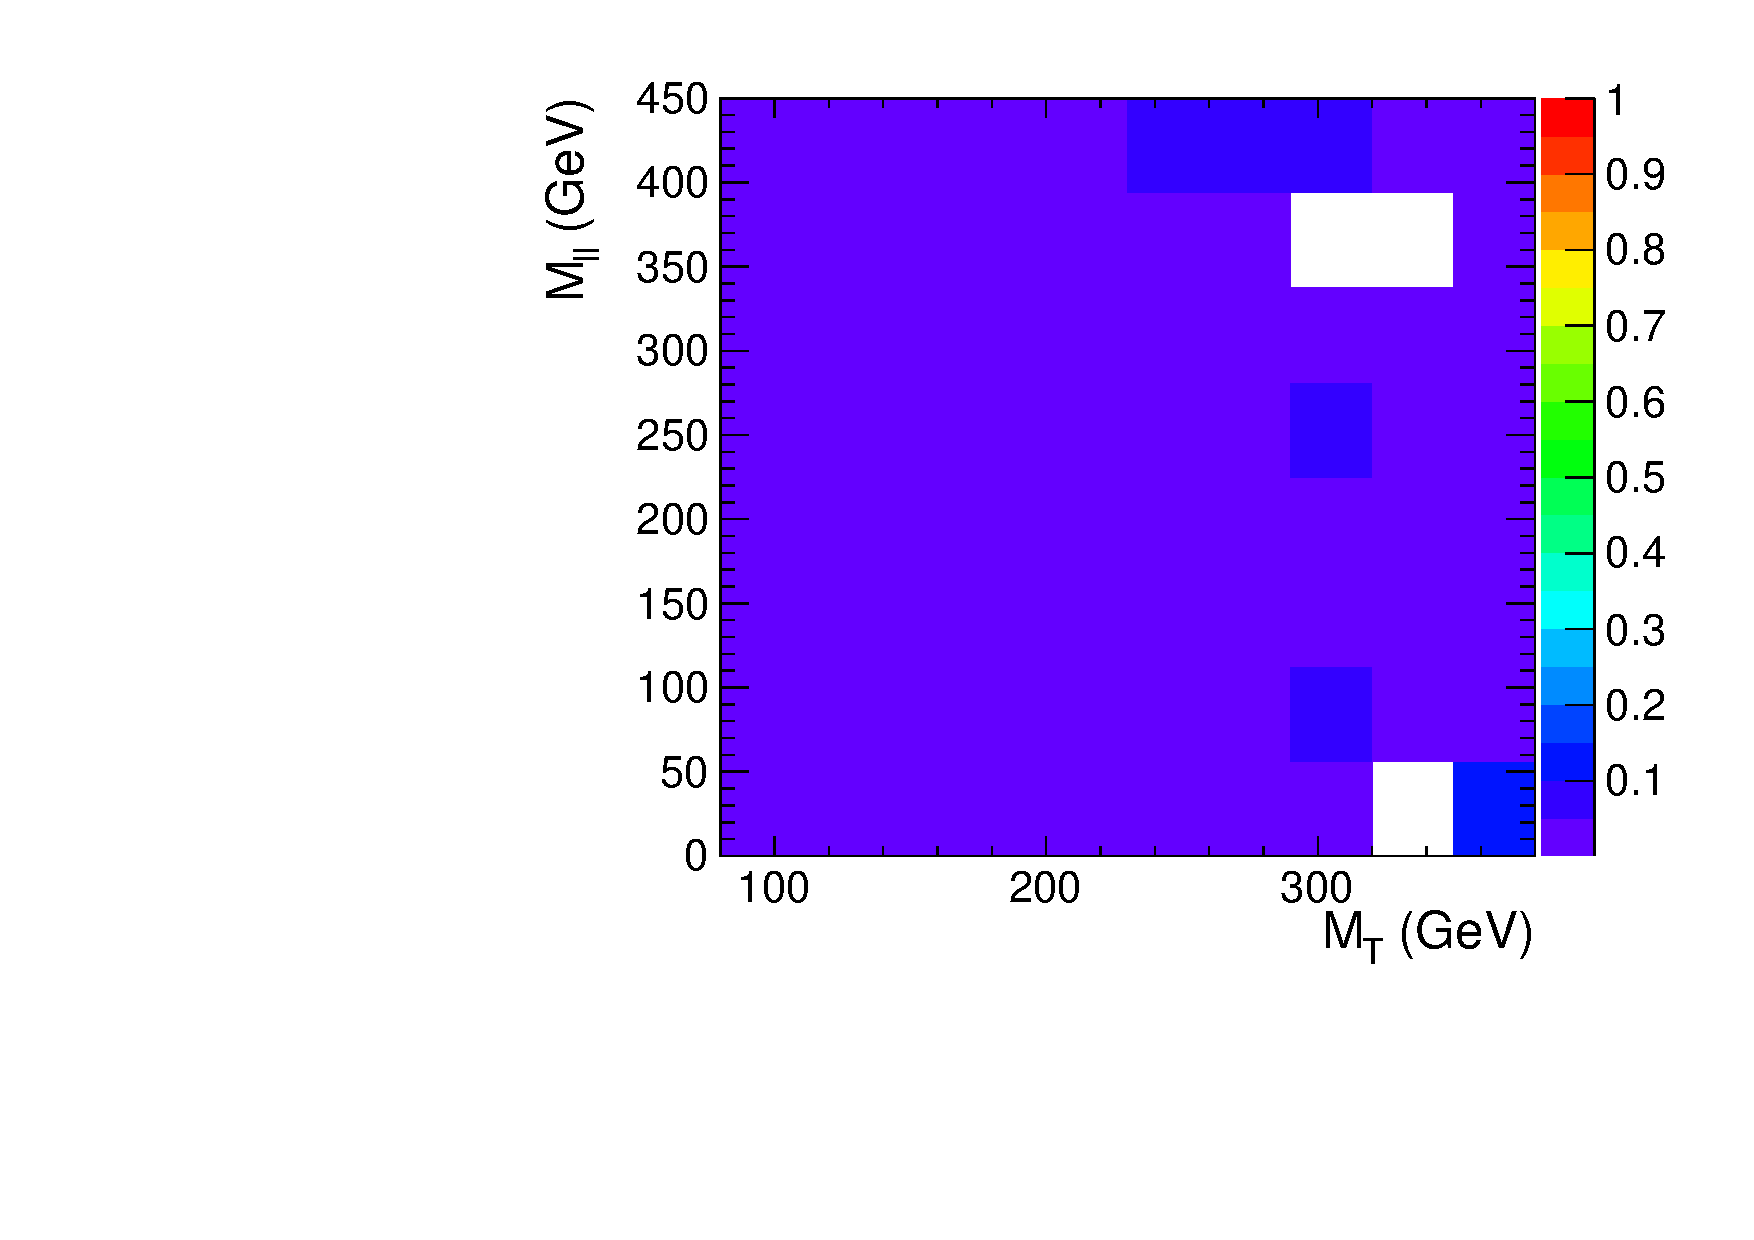
\includegraphics[width=.35\textwidth]{figures/templates/VVerr_2D_mH600_0j_of.pdf}
	}

	\caption{2D templates at \mHi = 600 \GeV in 0jet bin.} 
	\label{fig:templates_600_0j_2}

\end{figure}

\begin{figure}[!hbtp]
	
	%
	\centering
	\subfigure[Zjets]{
	\centering
	\label{subfig:template_Zjets_600}
		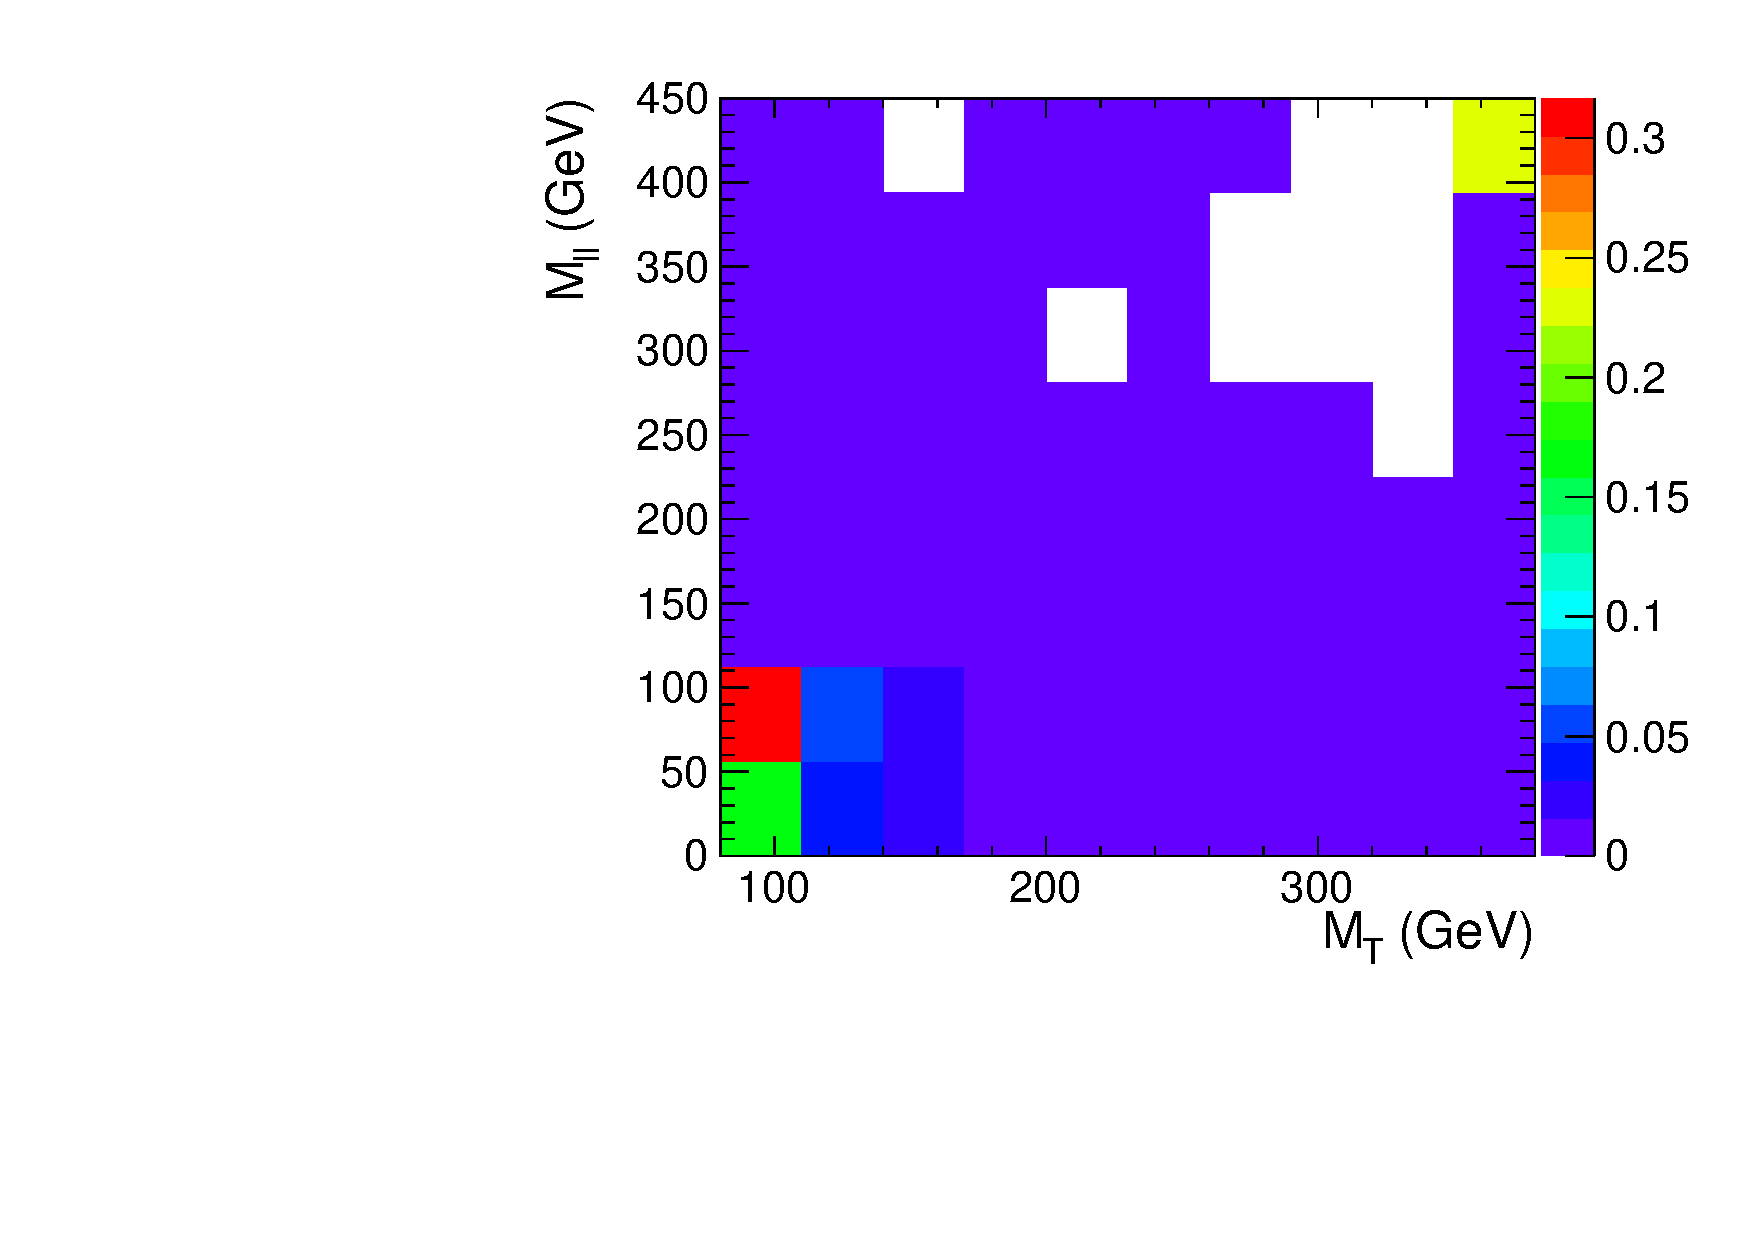
\includegraphics[width=.35\textwidth]{figures/templates/Zjets_2D_mH600_0j_of.pdf}
	}
	\subfigure[Zjets statistical uncertainty]{
	\centering
	\label{subfig:template_Zjetserr_600}
		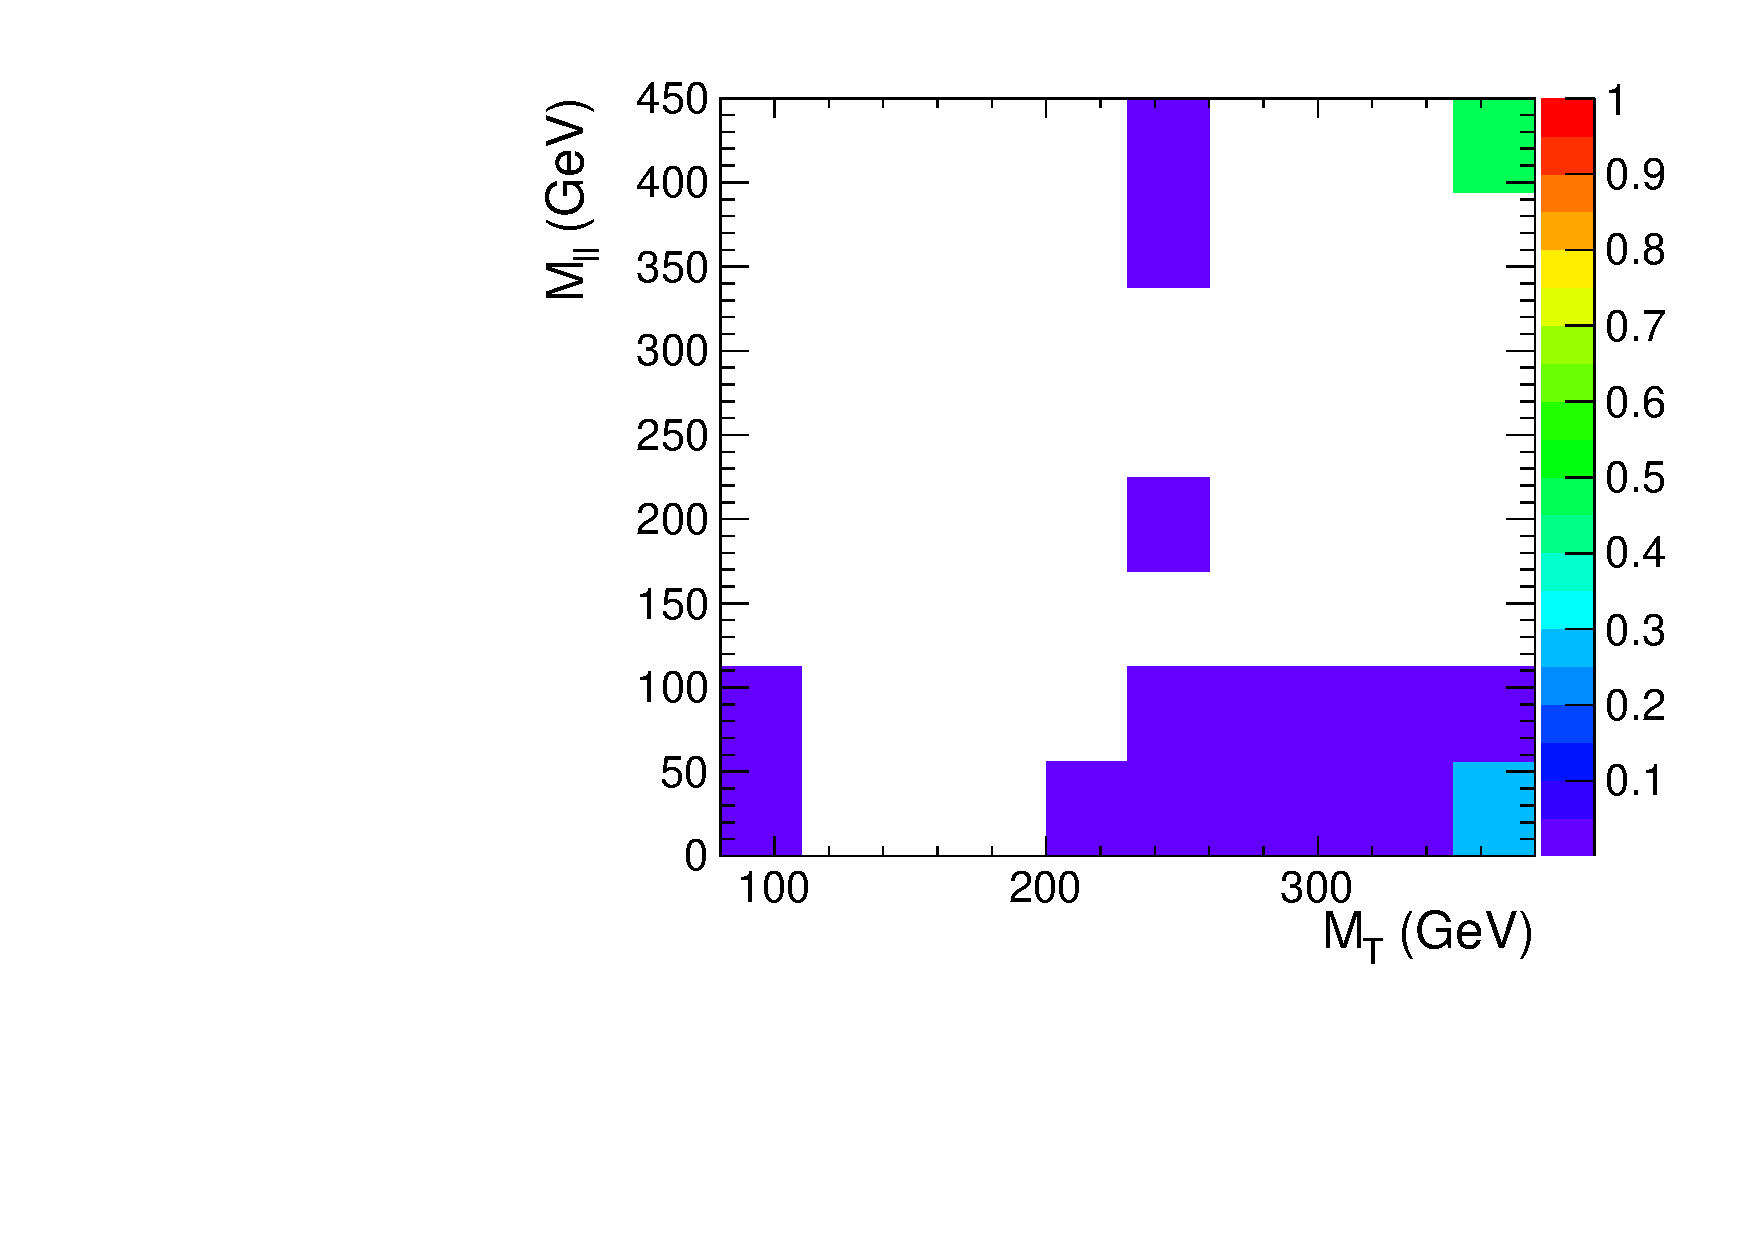
\includegraphics[width=.35\textwidth]{figures/templates/Zjetserr_2D_mH600_0j_of.pdf}
	}

	%
	\centering
	\subfigure[Wgamma]{
	\centering
	\label{subfig:template_Wgamma_600}
		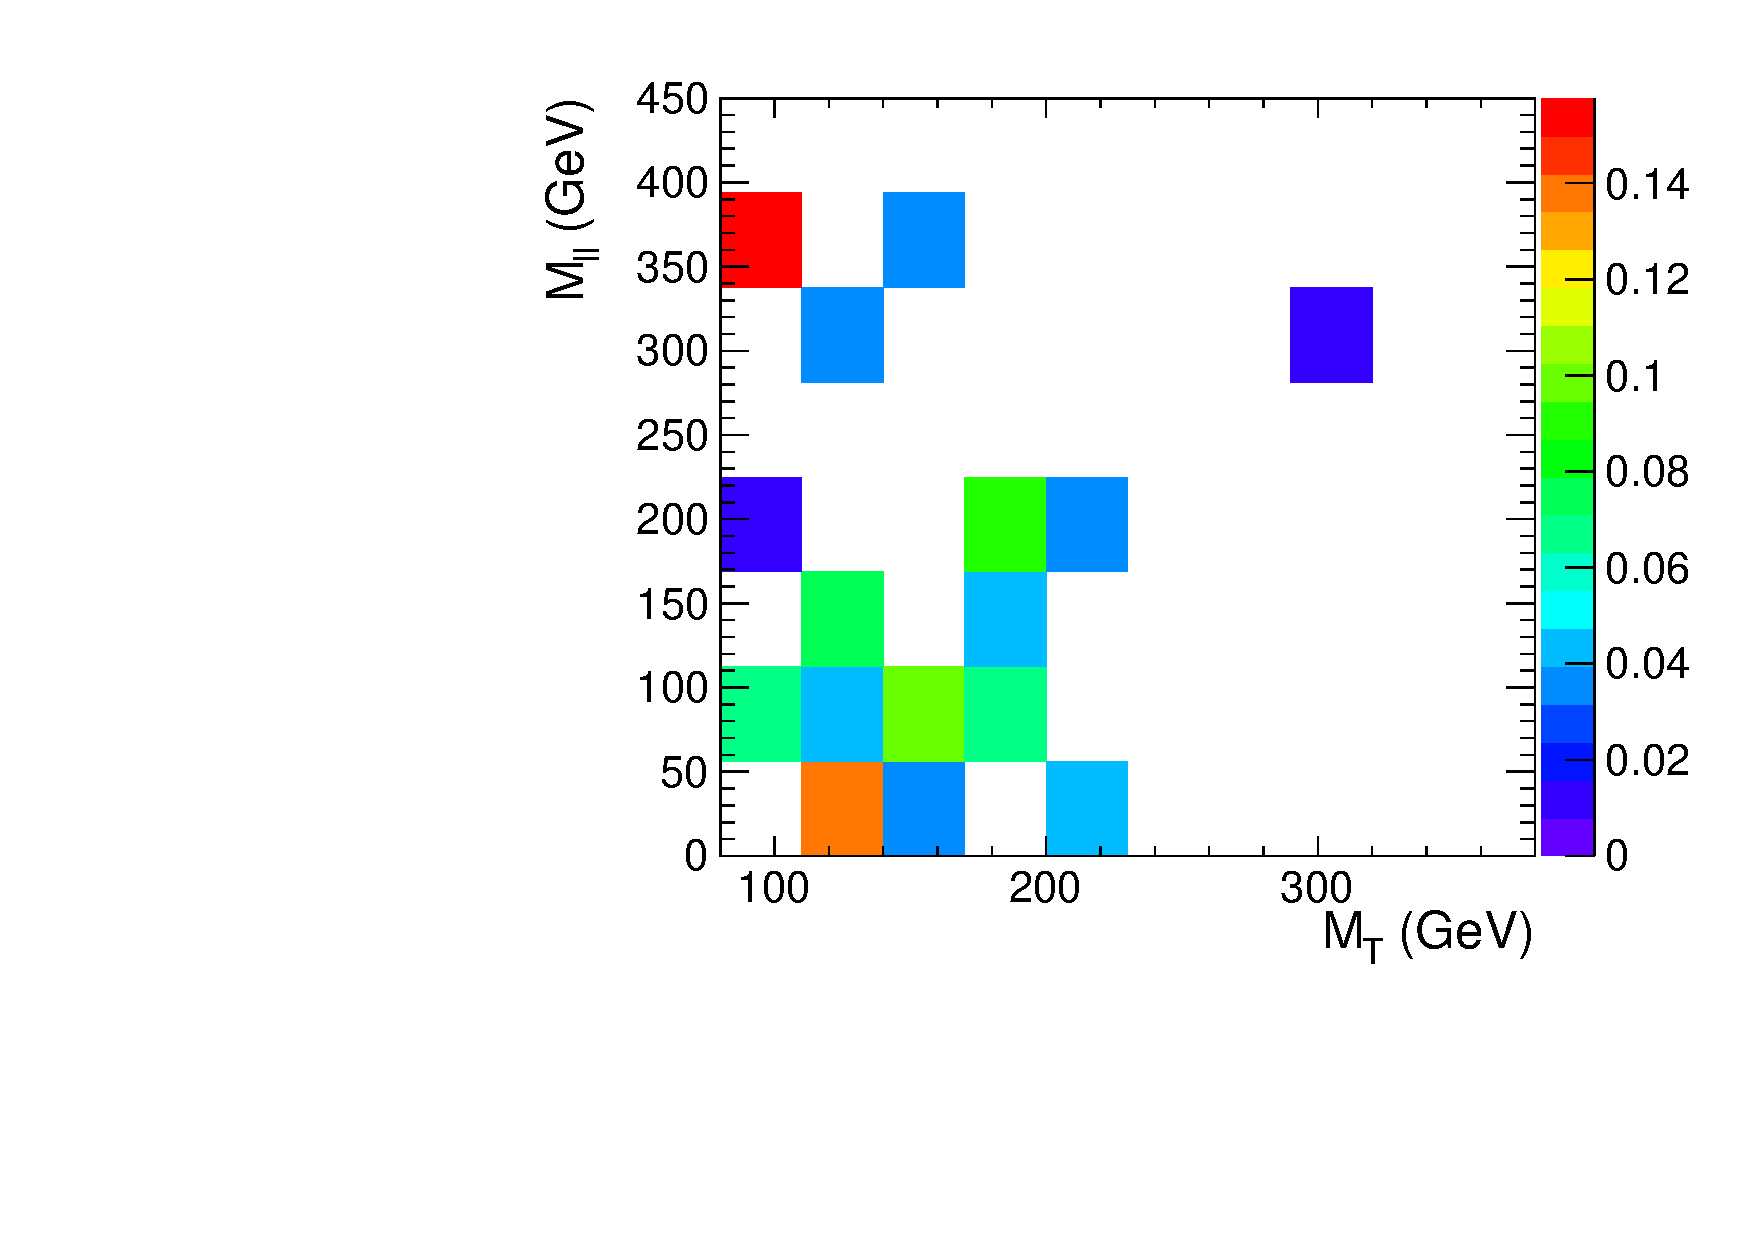
\includegraphics[width=.35\textwidth]{figures/templates/Wgamma_2D_mH600_0j_of.pdf}
	}
	\subfigure[Wgamma statistical uncertainty]{
	\centering
	\label{subfig:template_Wgammaerr_600}
		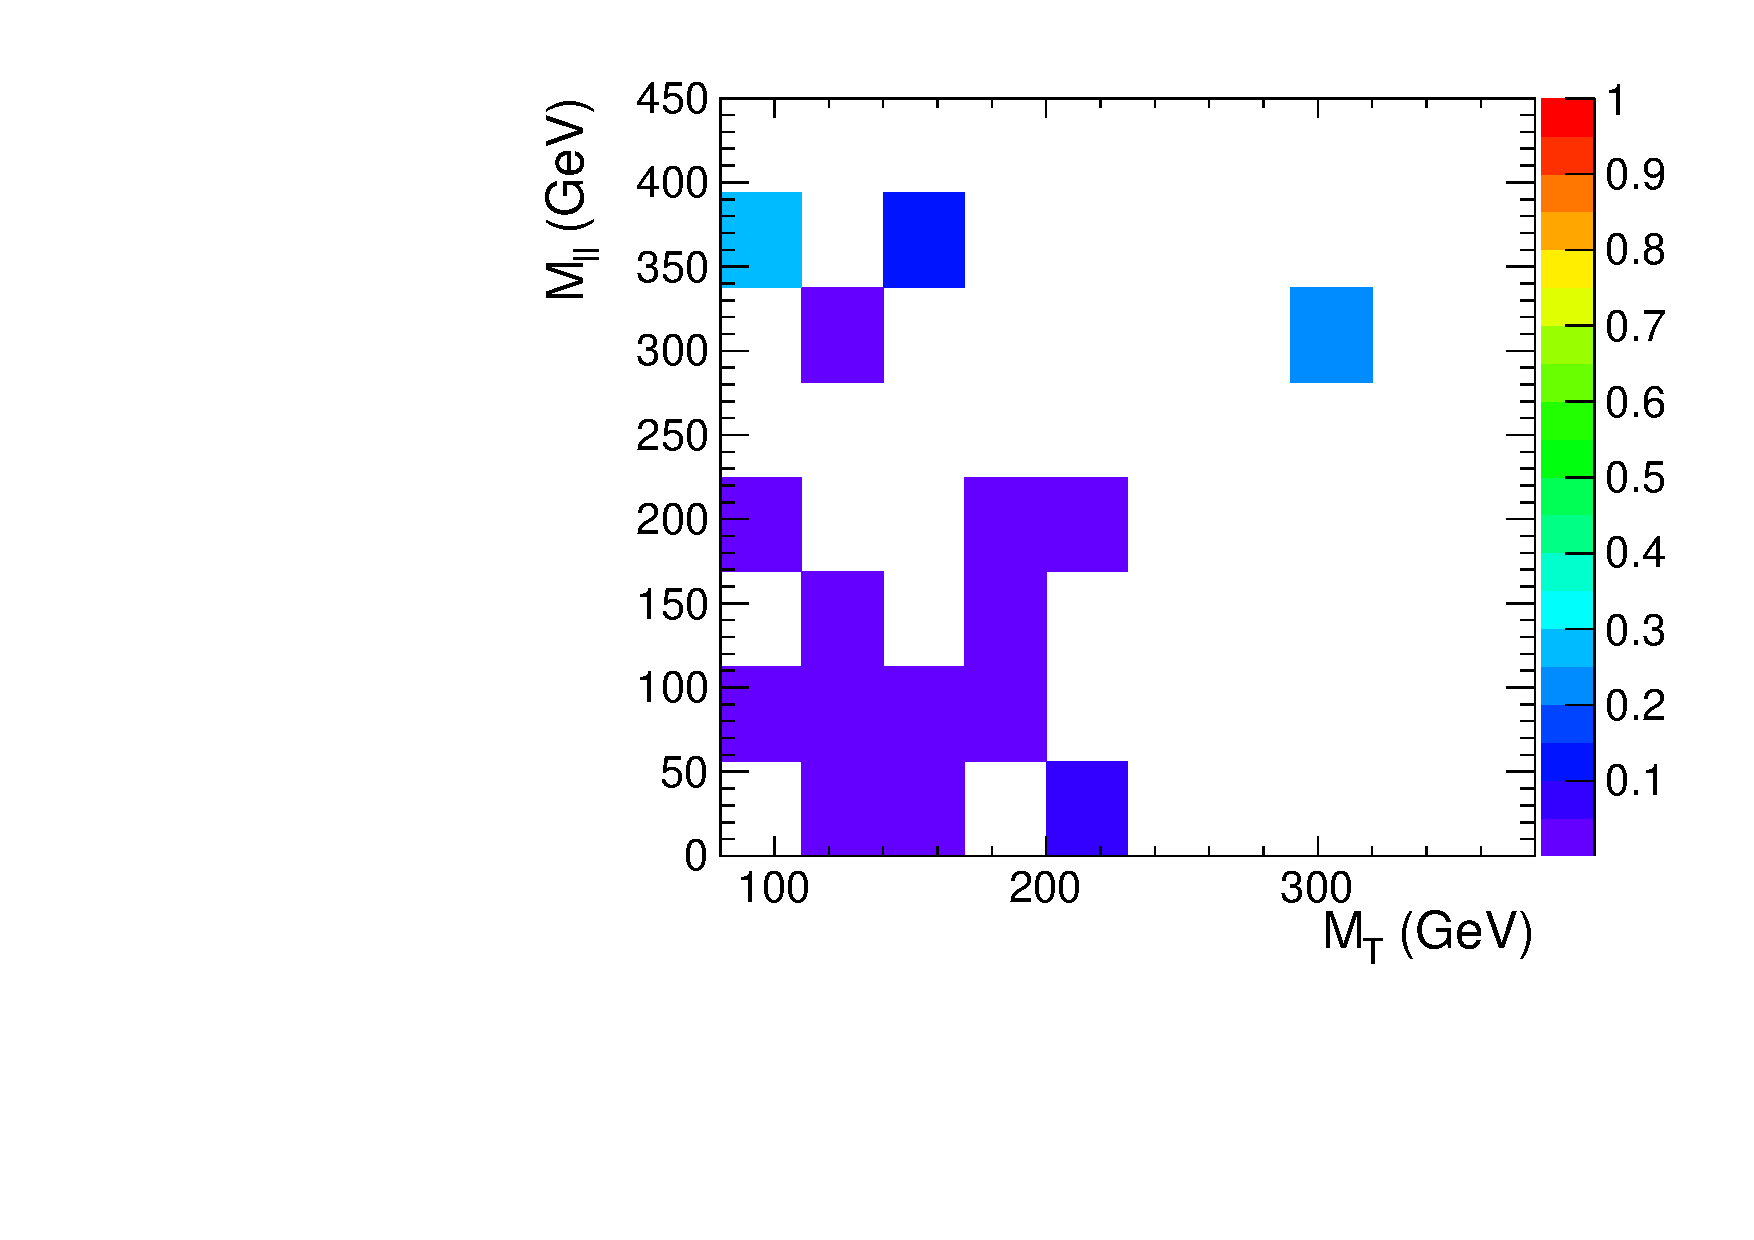
\includegraphics[width=.35\textwidth]{figures/templates/Wgammaerr_2D_mH600_0j_of.pdf}
	}

	\caption{2D templates at \mHi = 600 \GeV in 0jet bin.} 
	\label{fig:templates_600_0j_3}

\end{figure} 

\begin{figure}[!hbtp]
	
	%
	\centering
	\subfigure[Stacked unrolled template linear]{
	\centering
	\label{subfig:template_unroll_stack_lin}
		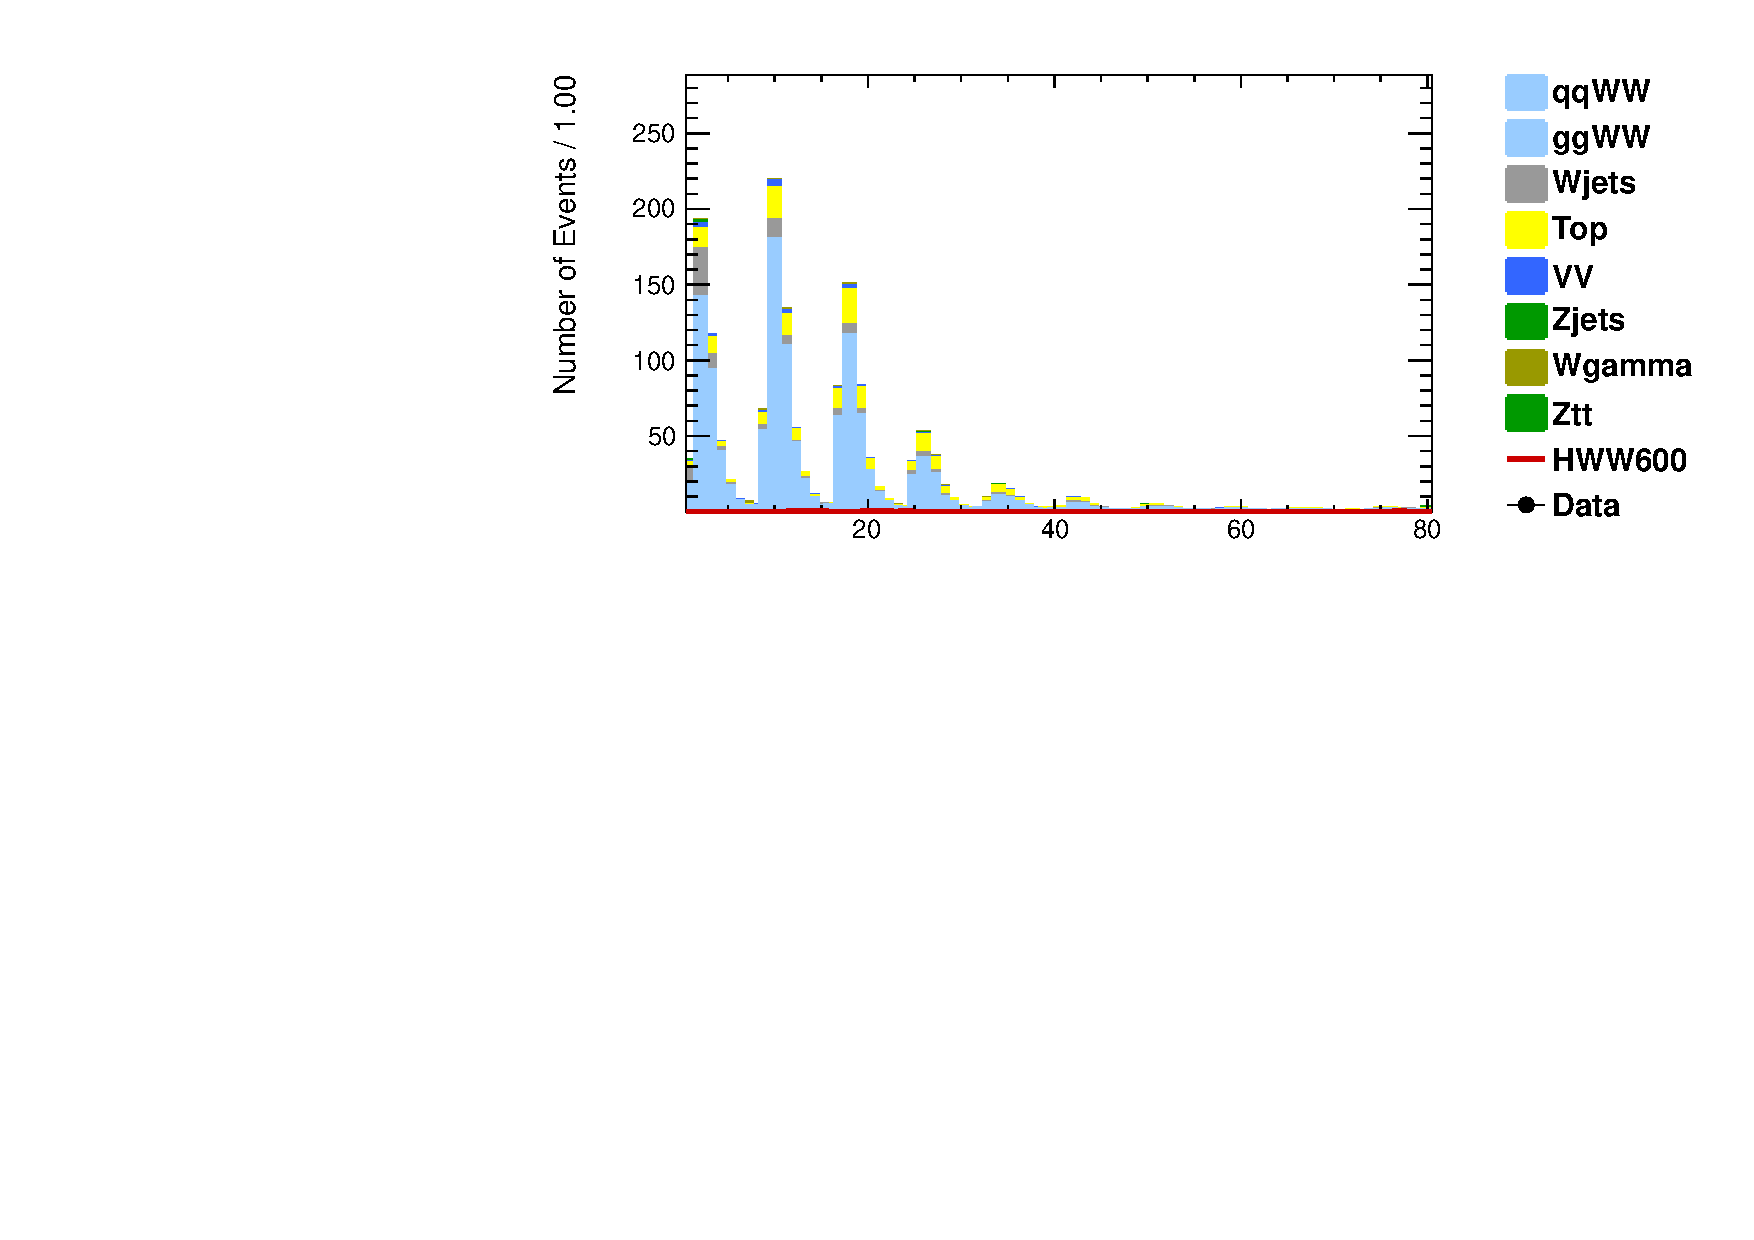
\includegraphics[width=.45\textwidth]{figures/templates/2D_mH600_0j_of_stack_lin.pdf}
	}
	\subfigure[Overlaid unrolled template linear]{
	\centering
	\label{subfig:template_unroll_overlay_lin}
		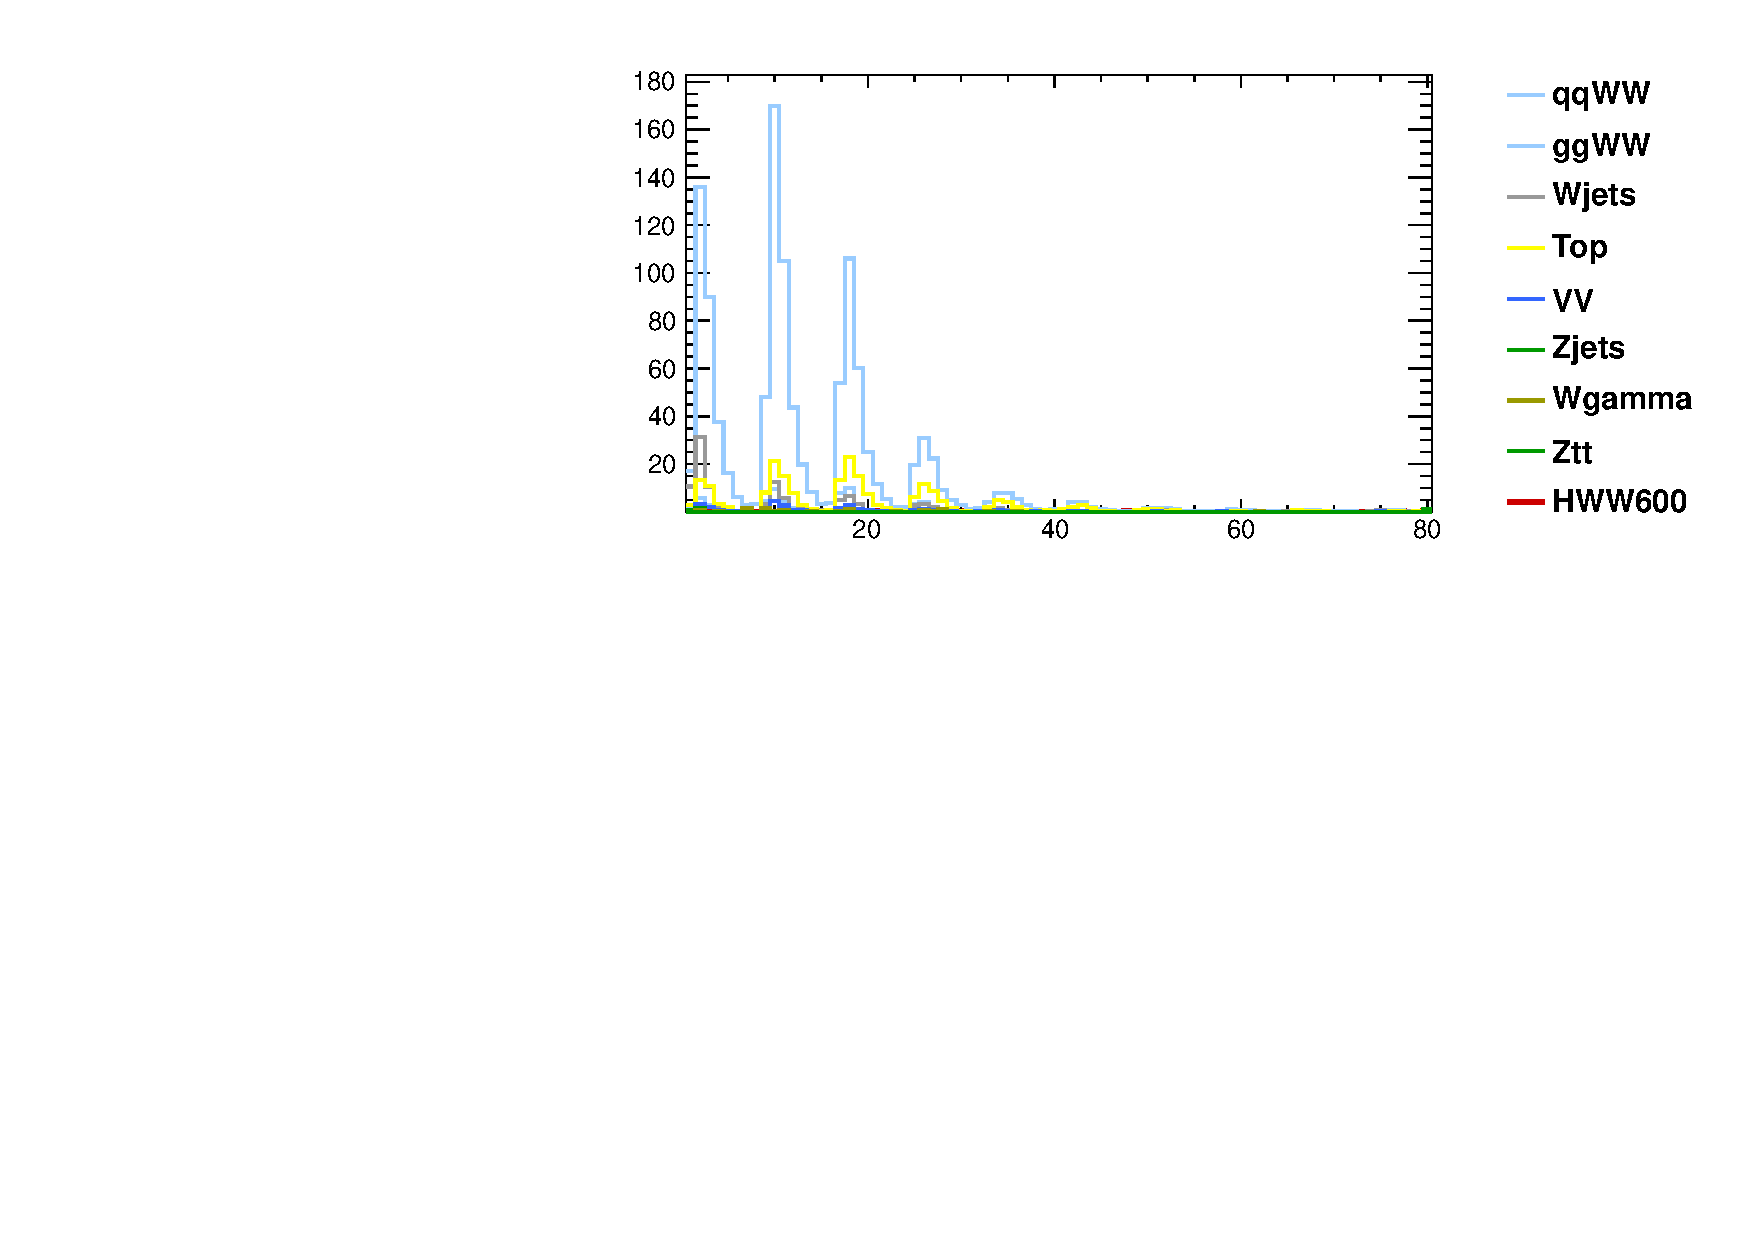
\includegraphics[width=.45\textwidth]{figures/templates/2D_mH600_0j_of_overlay_lin.pdf}
	}

	%
	\centering
	\subfigure[Stacked unrolled template in log scale]{
	\centering
	\label{subfig:template_unroll_stack_log}
		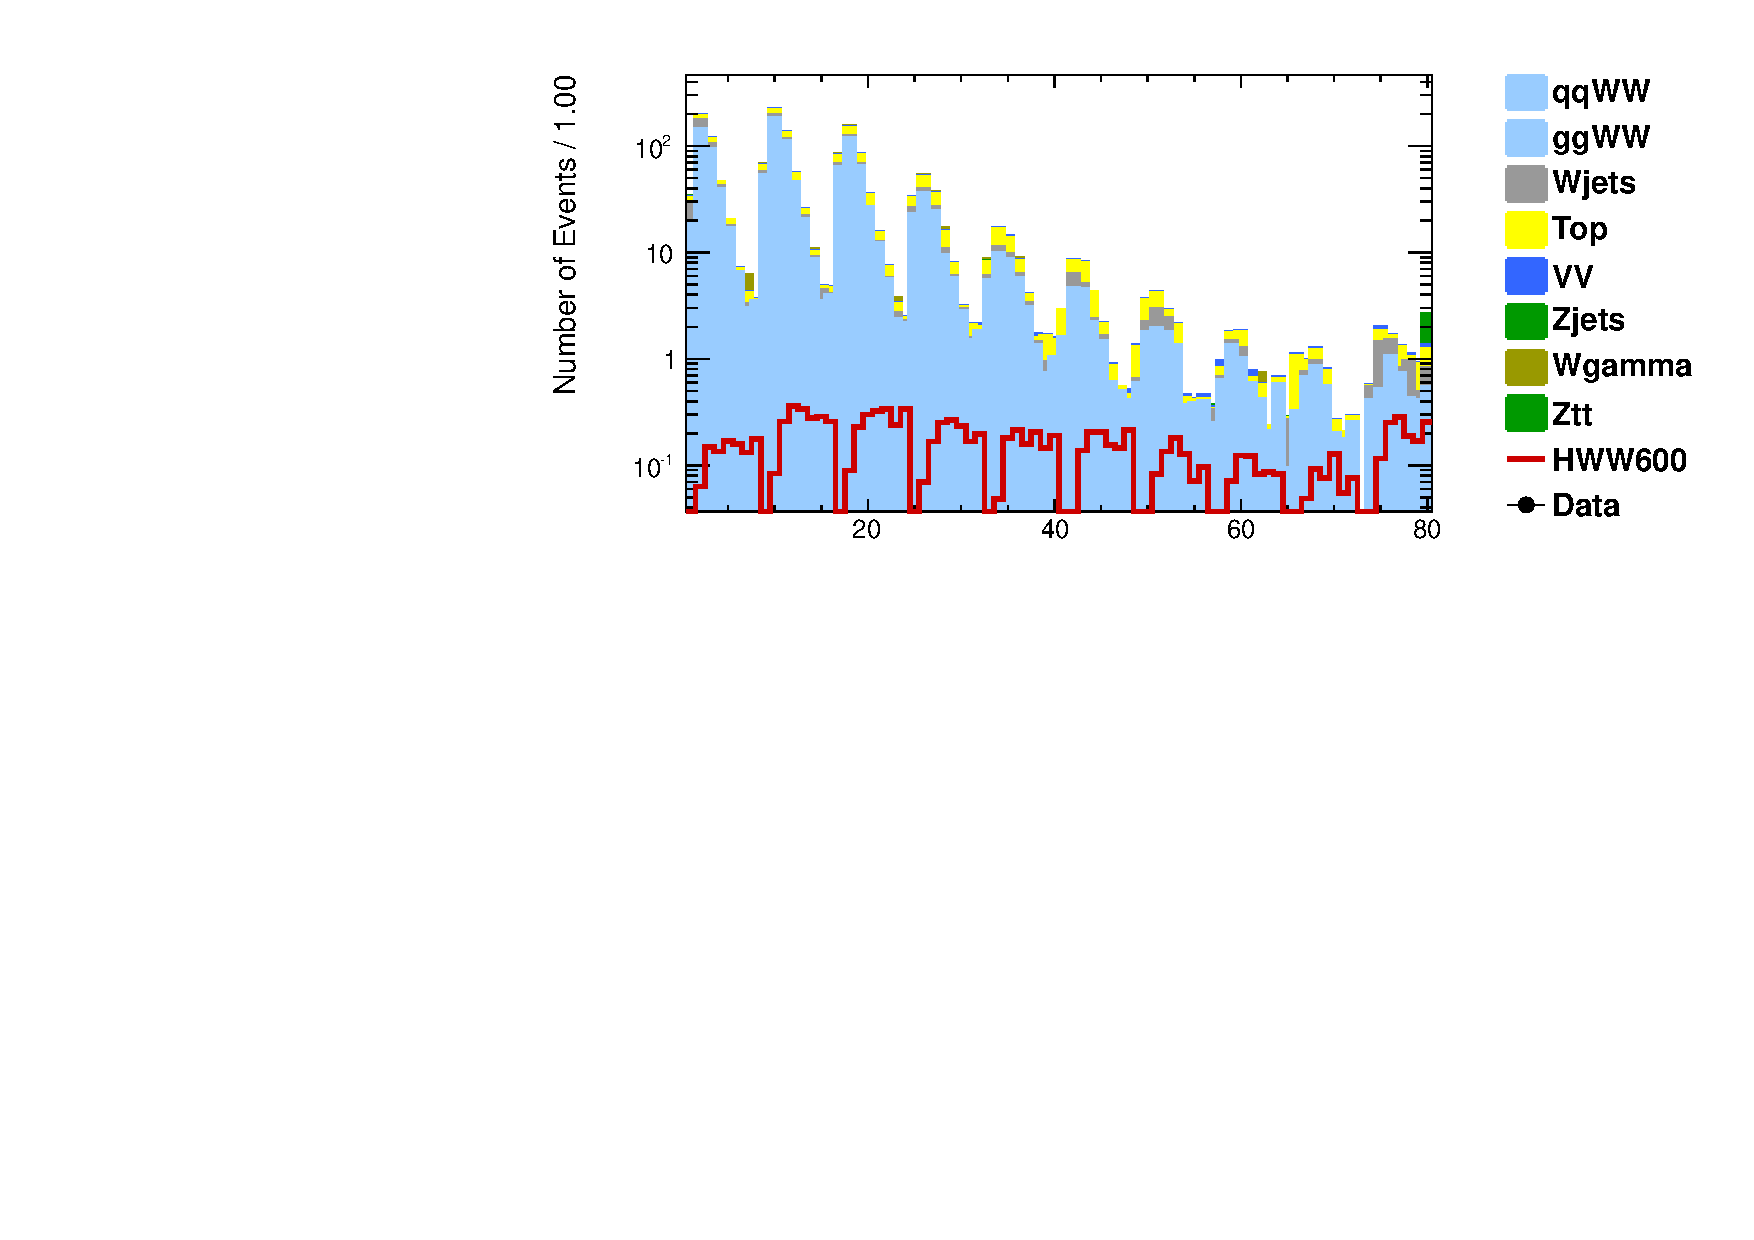
\includegraphics[width=.45\textwidth]{figures/templates/2D_mH600_0j_of_stack_log.pdf}
	}
	\subfigure[Overlaid unrolled template in log scale]{
	\centering
	\label{subfig:template_unroll_overlay_log}
		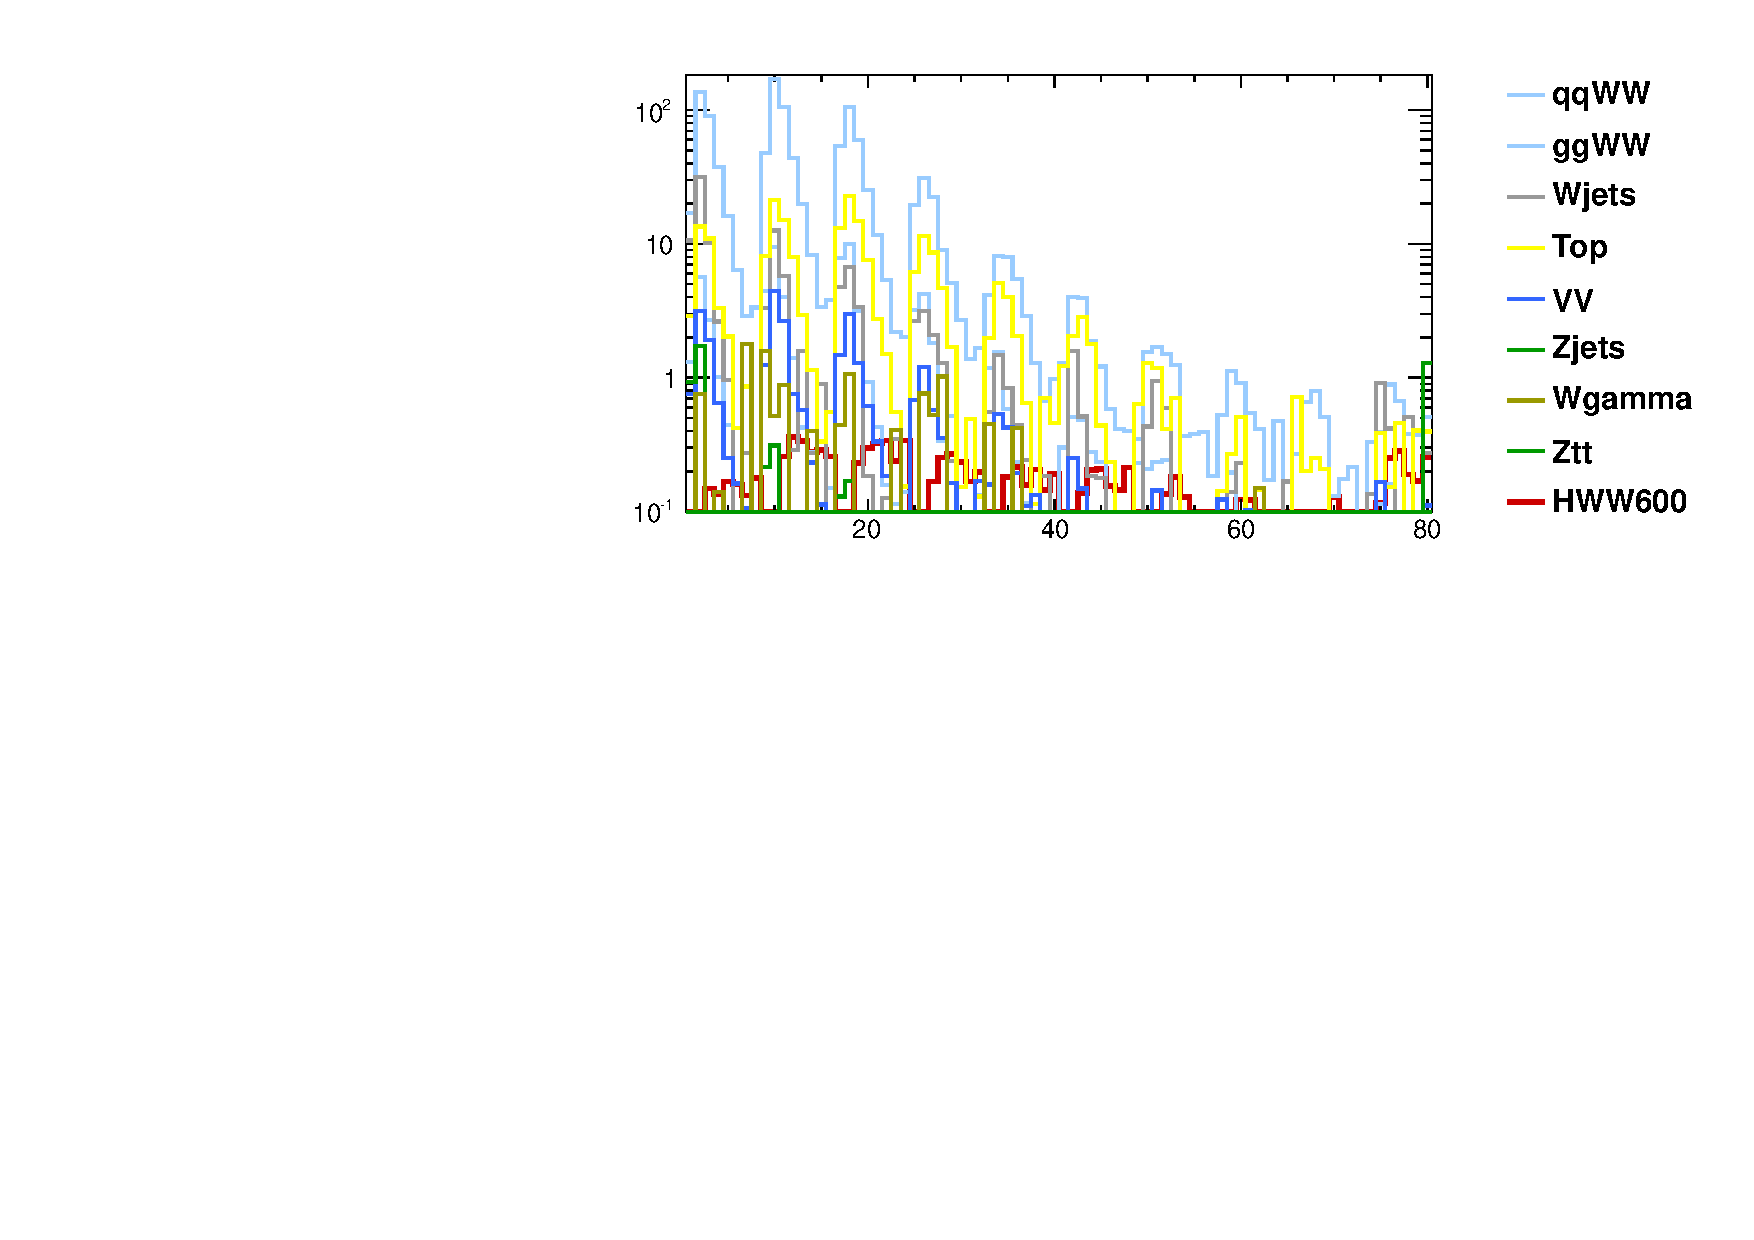
\includegraphics[width=.45\textwidth]{figures/templates/2D_mH600_0j_of_overlay_log.pdf}
	}

	\caption{Unrolled templates at \mHi = 600 \GeV in 0jet bin.} 
	\label{fig:templates_600_0j_unroll}

\end{figure} 

\newpage
%%% mH=125 VBF 
\begin{figure}[!hbtp]
	
	%
	\centering
	\subfigure[Signal]{
	\centering
	\label{subfig:template_signal_125}
		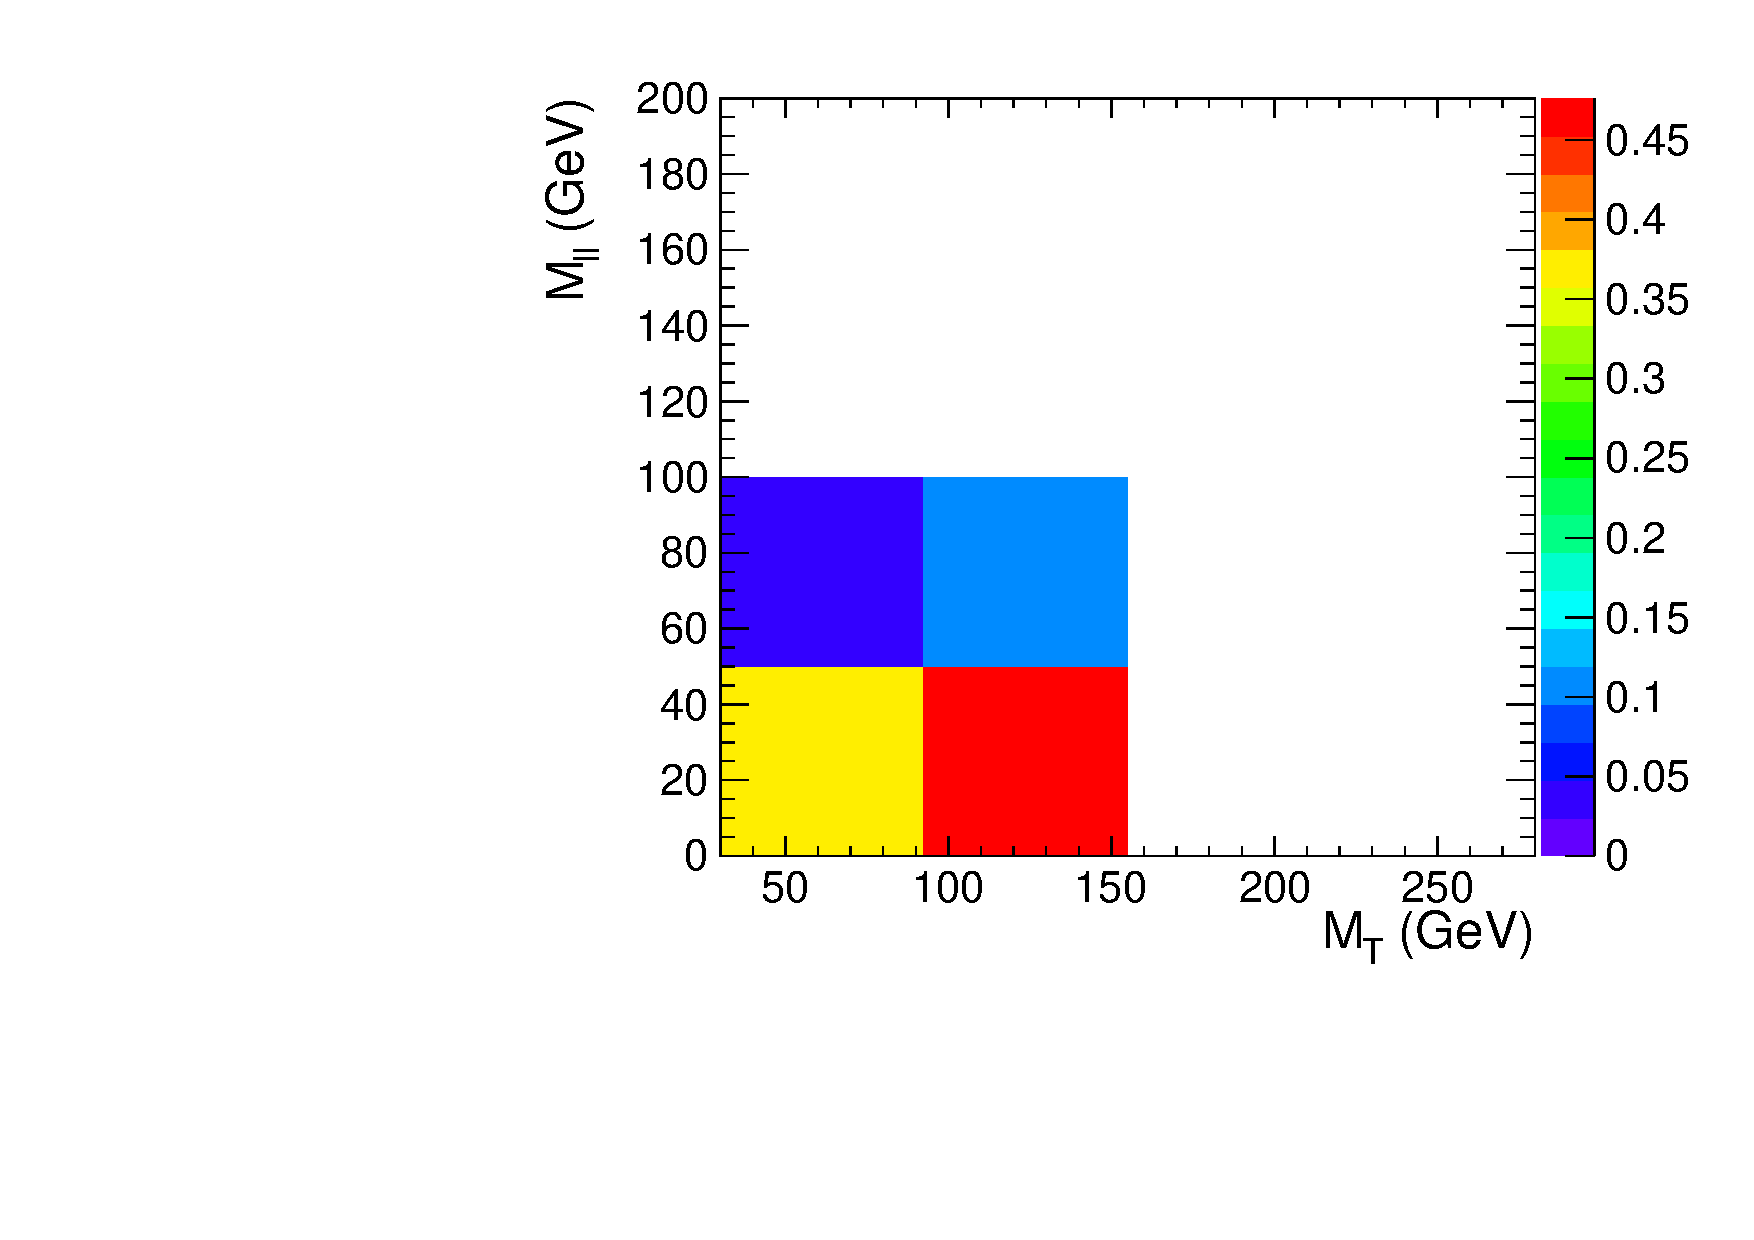
\includegraphics[width=.35\textwidth]{figures/templates/sig_2D_mH125_2j_of.pdf}
	}
	\subfigure[Signal statistical uncertainty]{
	\centering
	\label{subfig:template_signalerr_125}
		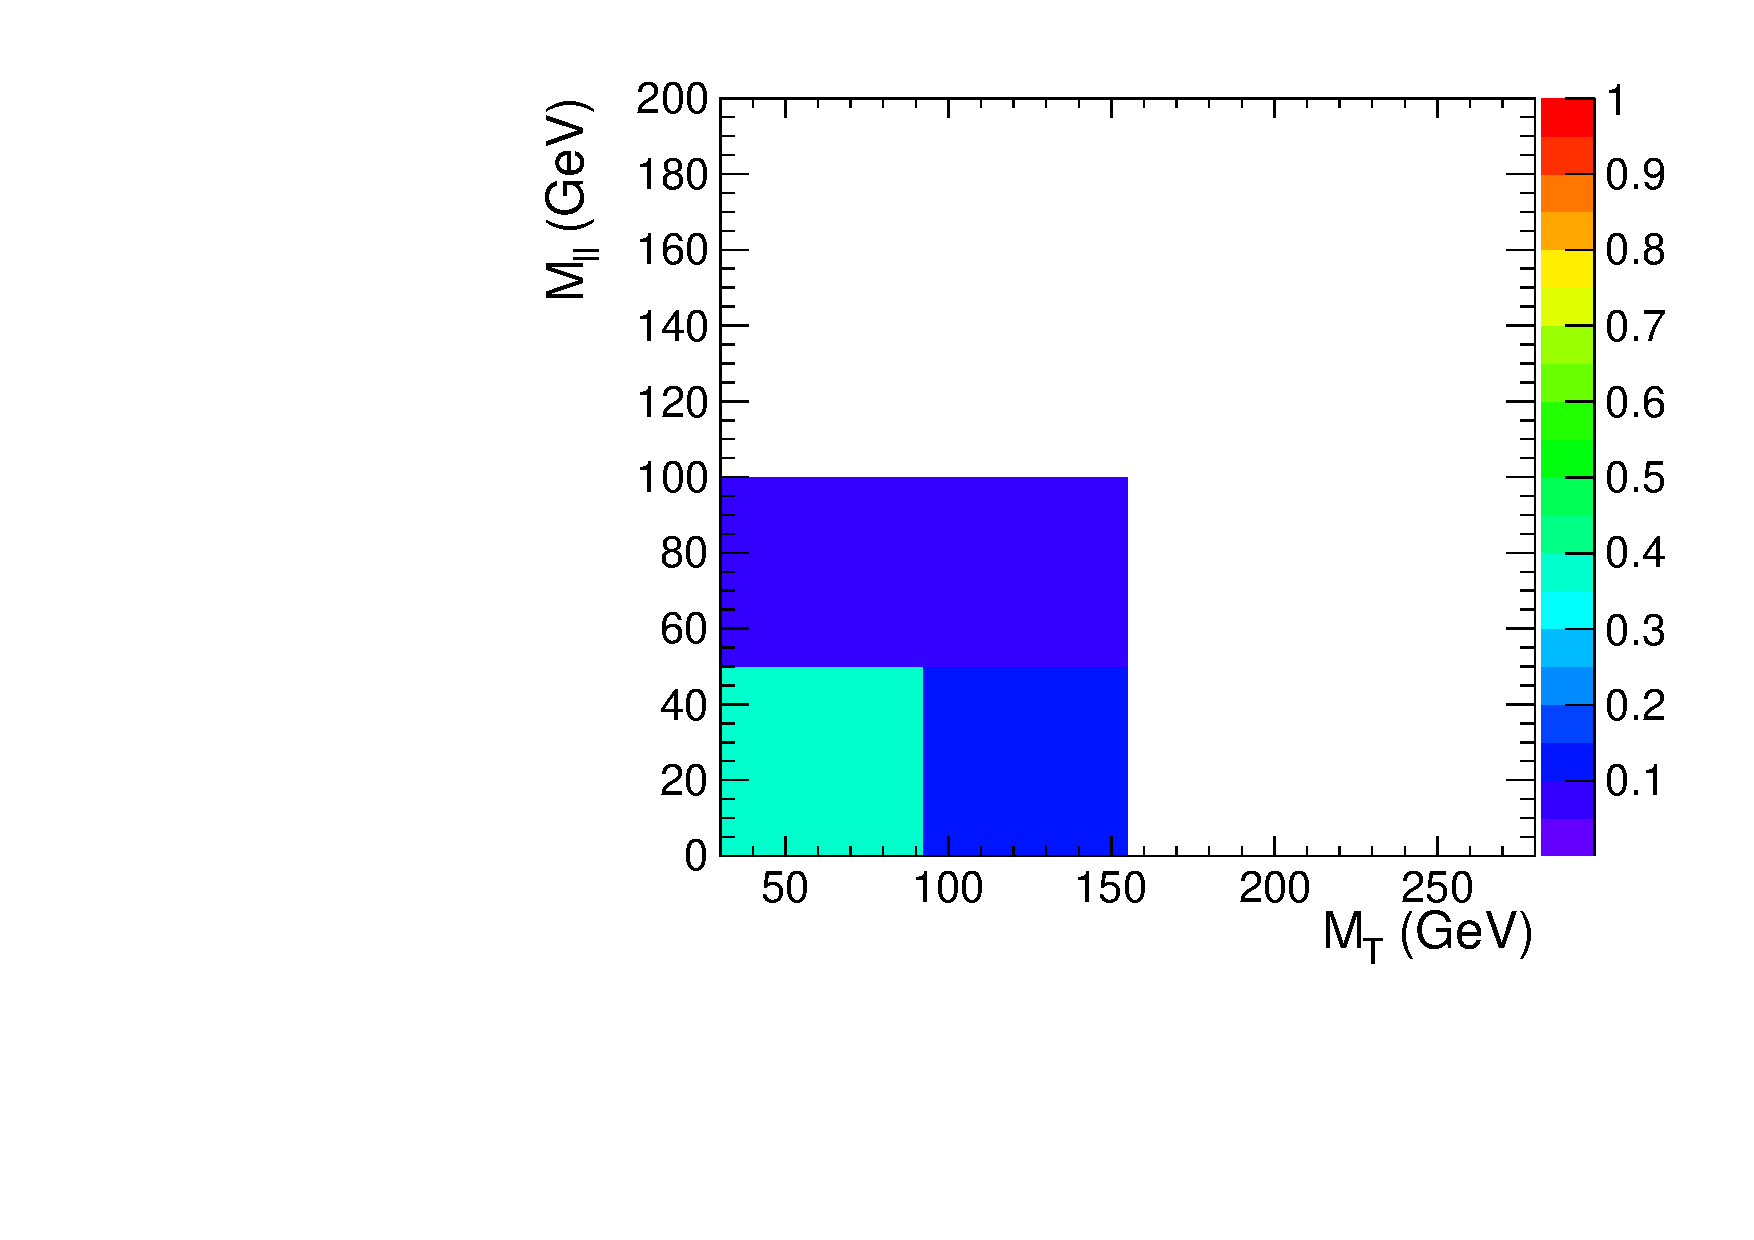
\includegraphics[width=.35\textwidth]{figures/templates/sigerr_2D_mH125_2j_of.pdf}
	}
	
	%
	\centering
	\subfigure[qqWW]{
	\centering
	\label{subfig:template_qqWW_125}
		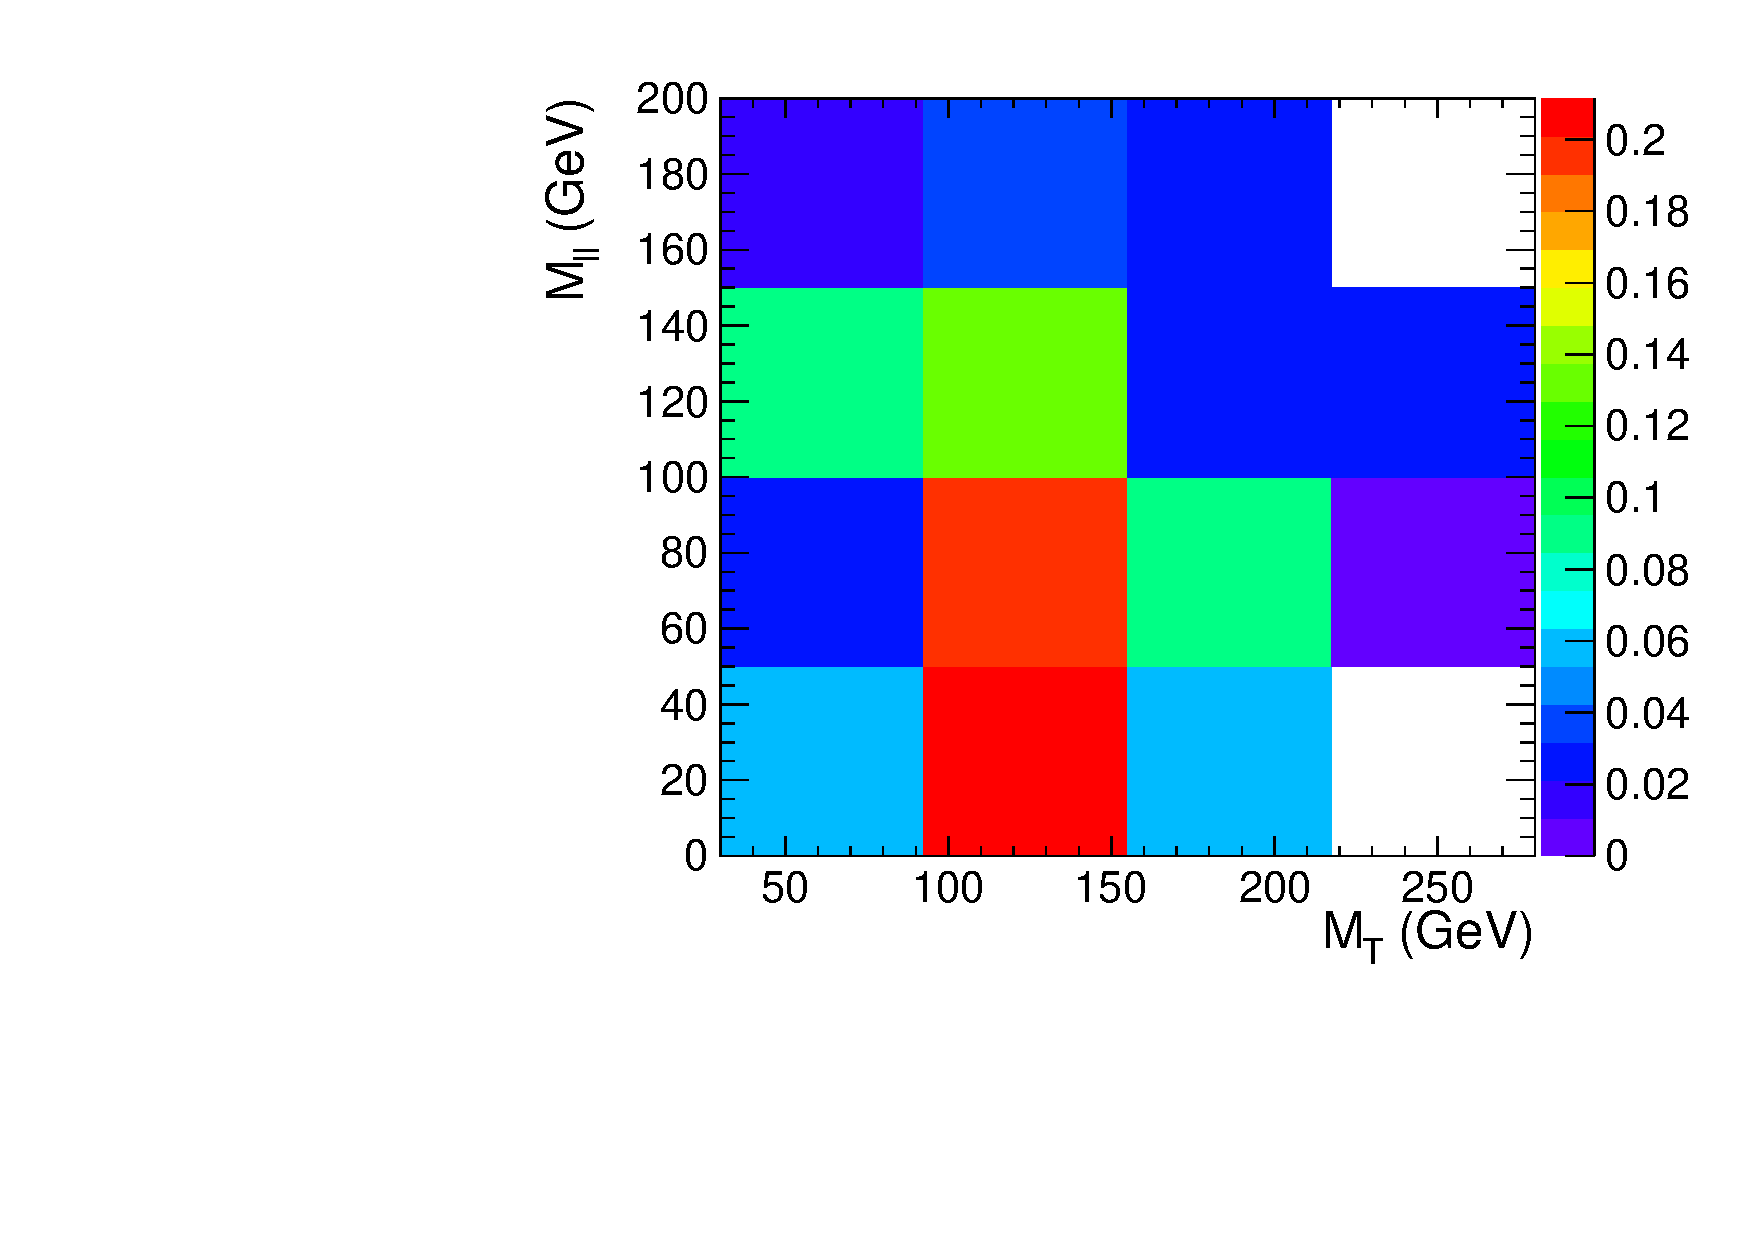
\includegraphics[width=.35\textwidth]{figures/templates/qqWW_2D_mH125_2j_of.pdf}
	}
	\subfigure[qqWW statistical uncertainty]{
	\centering
	\label{subfig:template_qqWWerr_125}
		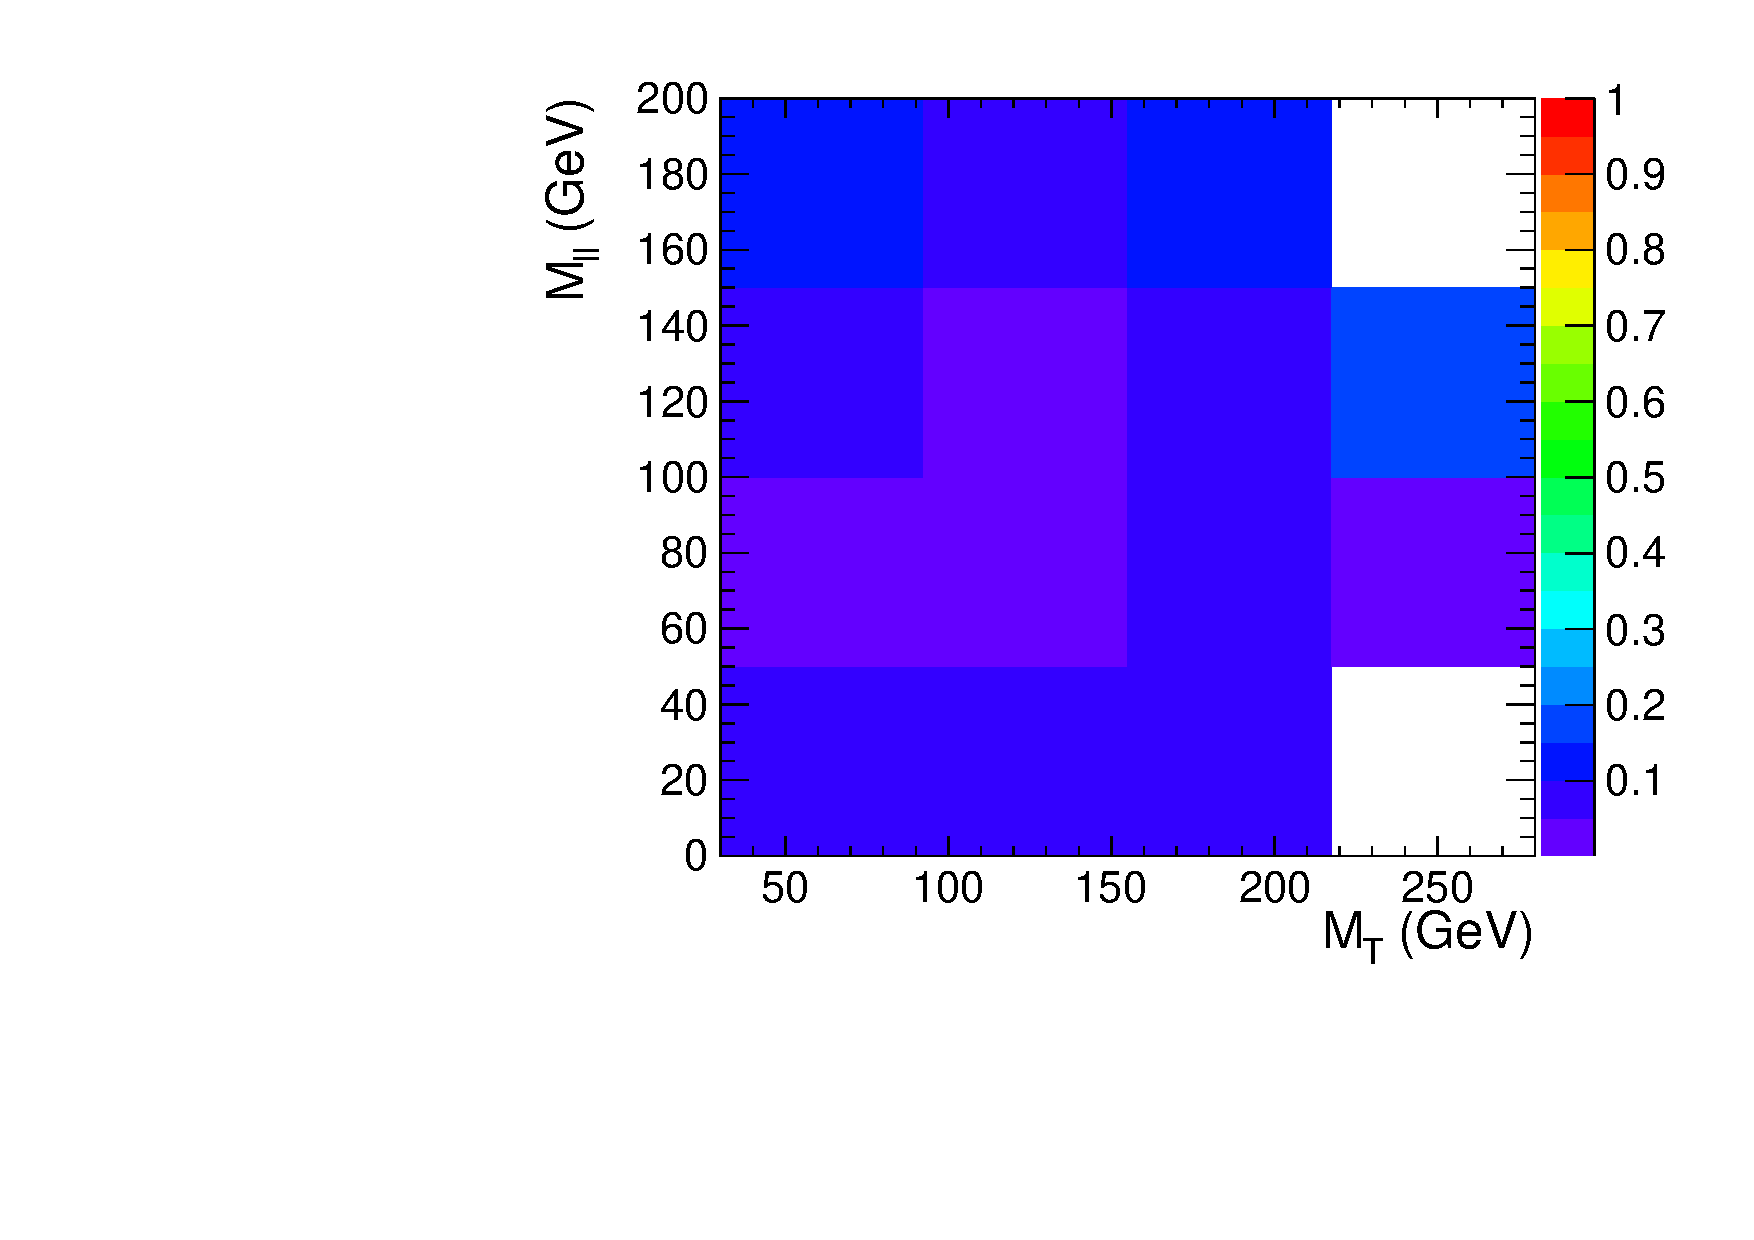
\includegraphics[width=.35\textwidth]{figures/templates/qqWWerr_2D_mH125_2j_of.pdf}
	}

	%
	\centering
	\subfigure[ggWW]{
	\centering
	\label{subfig:template_ggWW_125}
		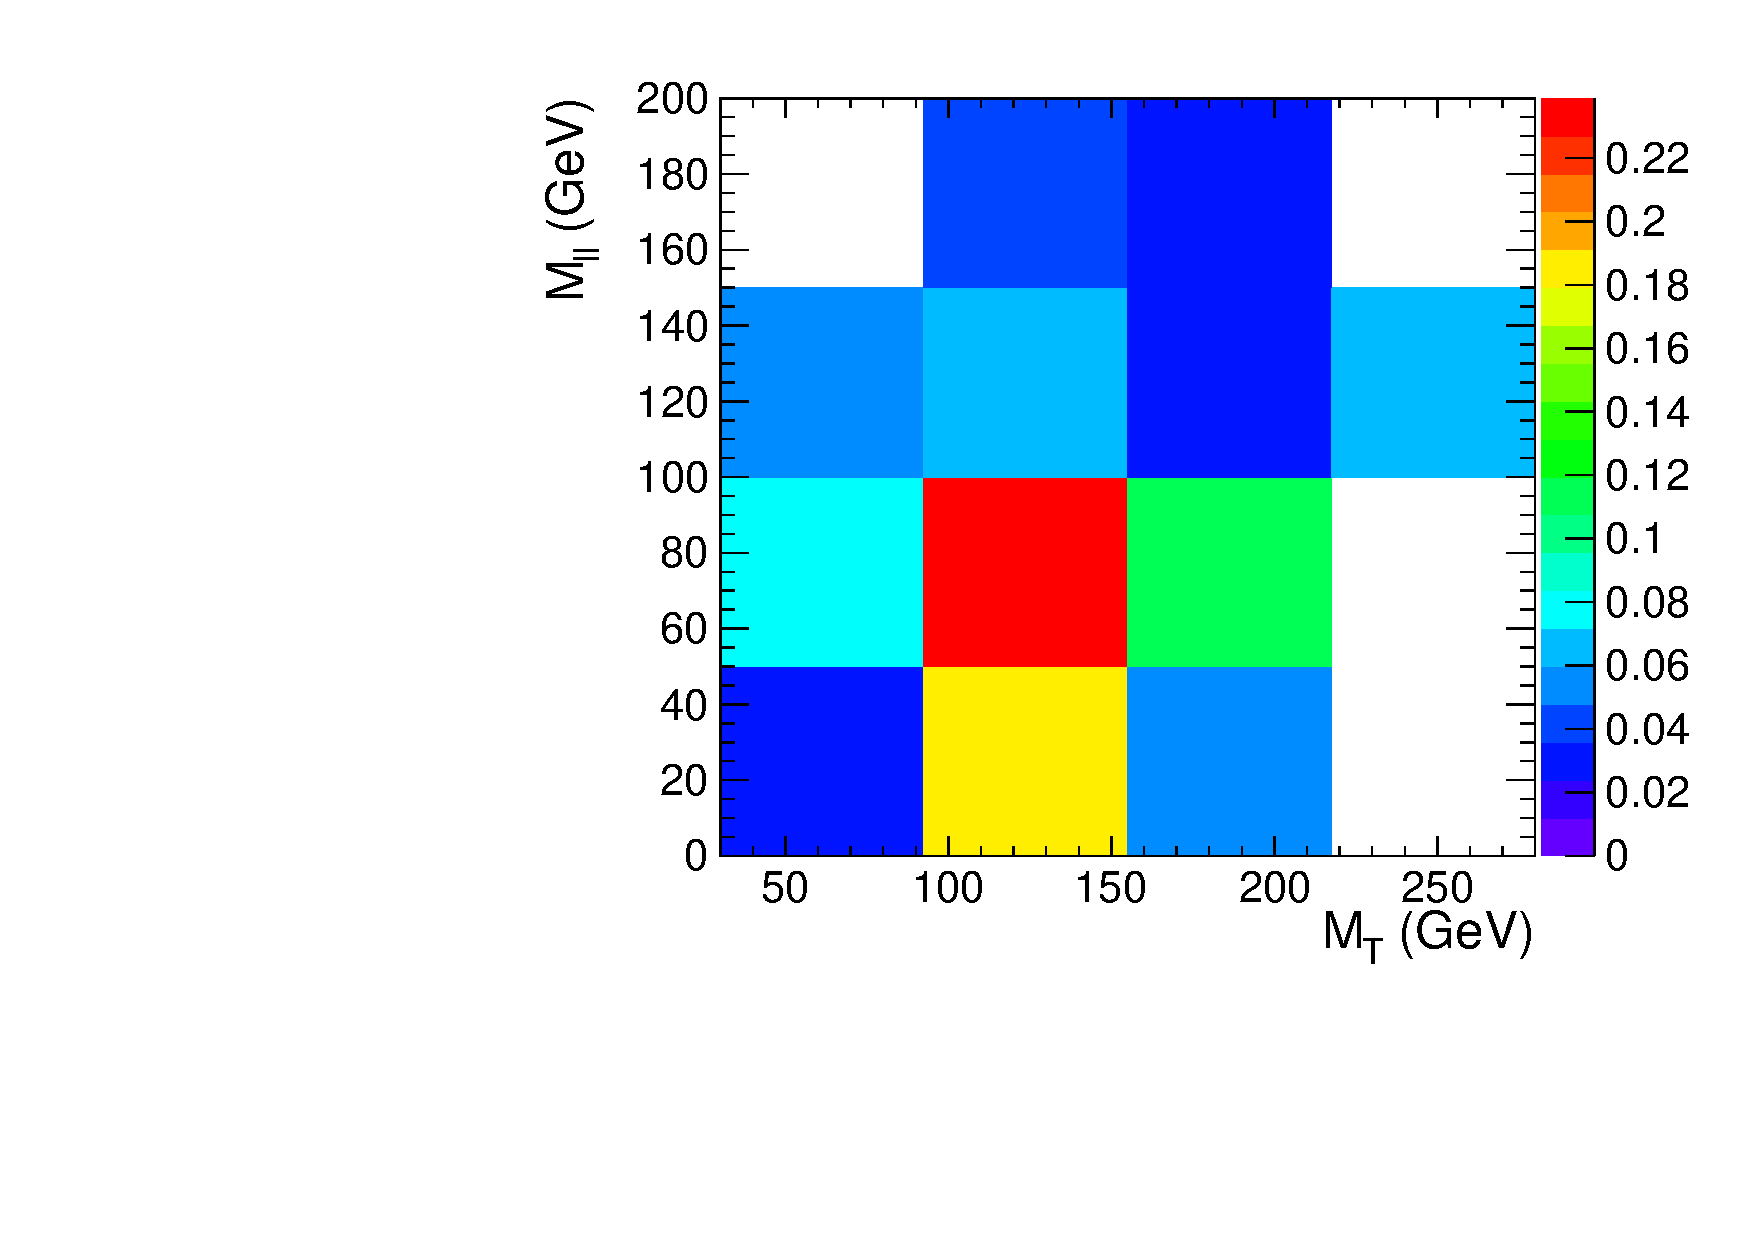
\includegraphics[width=.35\textwidth]{figures/templates/ggWW_2D_mH125_2j_of.pdf}
	}
	\subfigure[ggWW statistical uncertainty]{
	\centering
	\label{subfig:template_ggWWerr_125}
		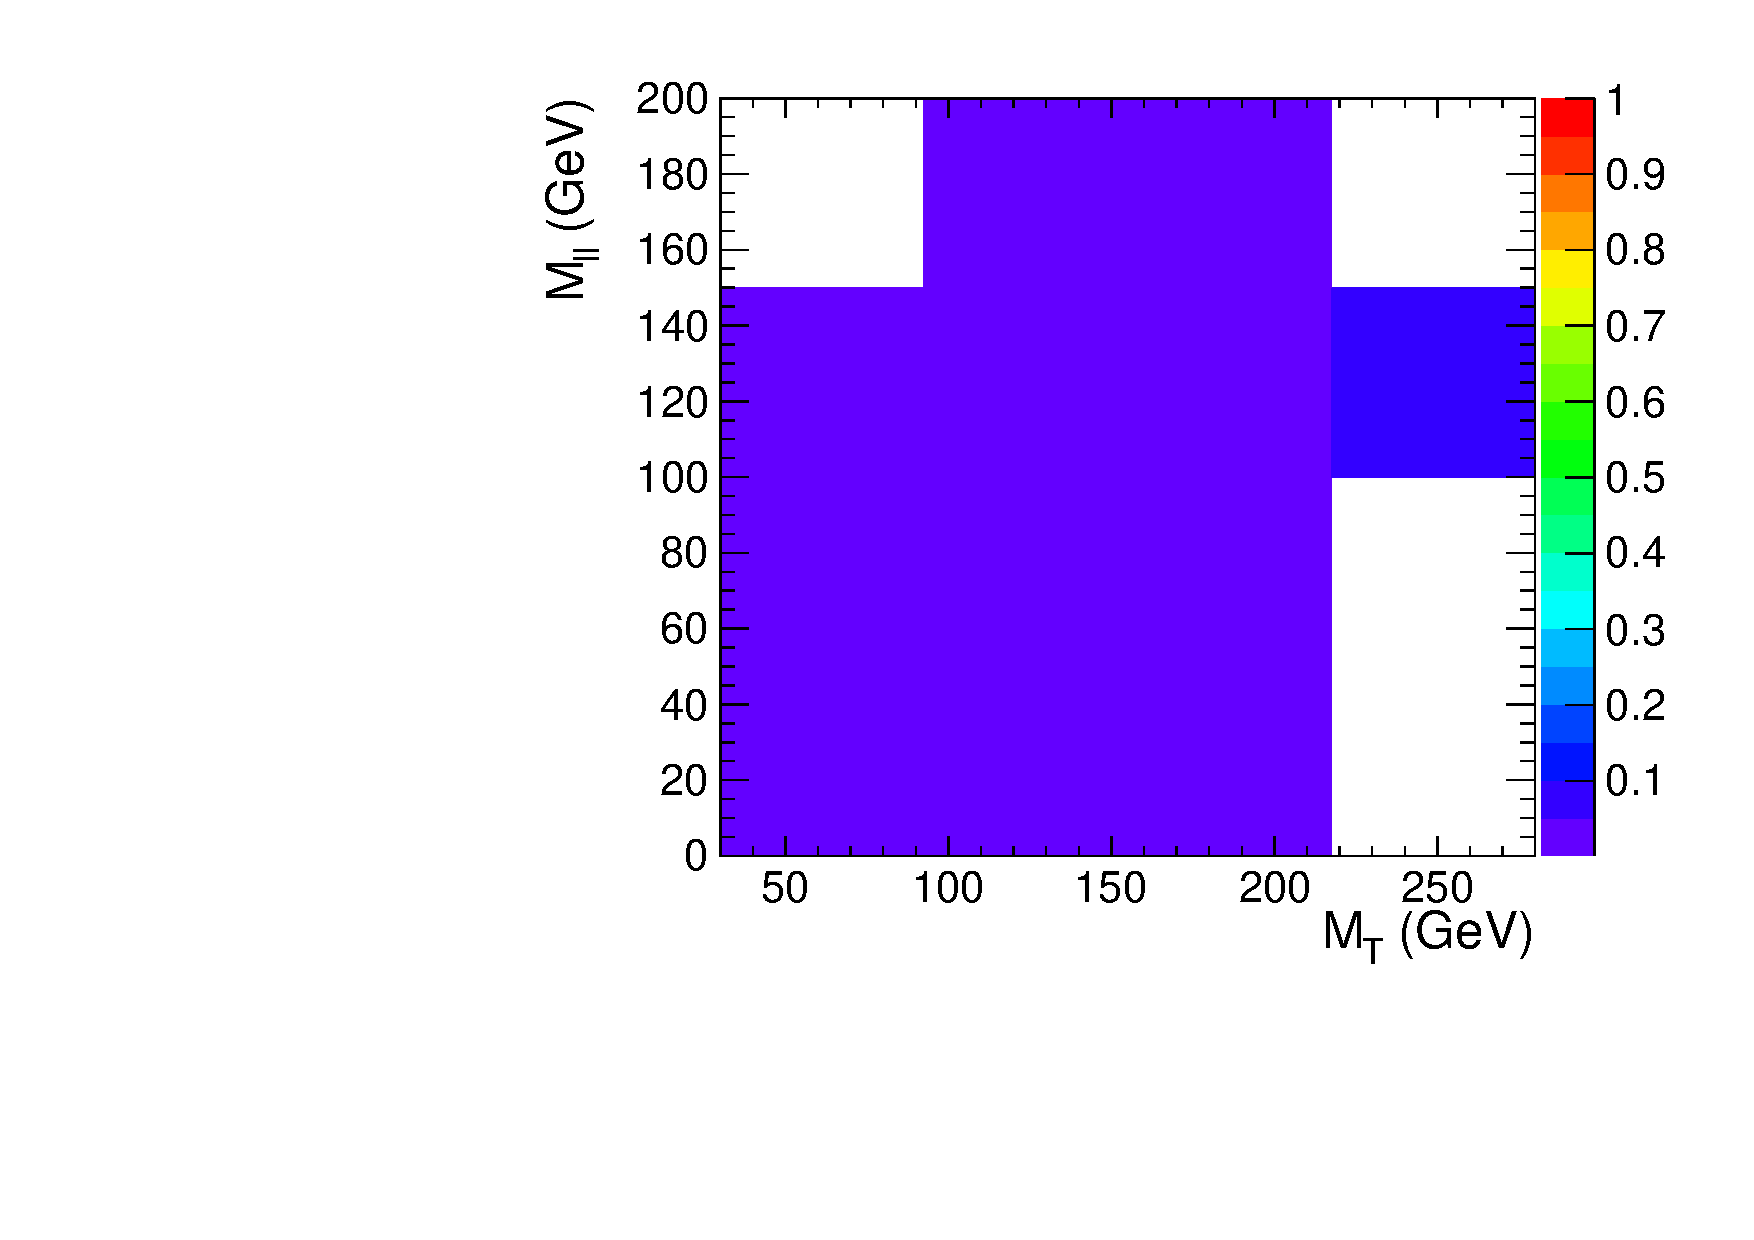
\includegraphics[width=.35\textwidth]{figures/templates/ggWWerr_2D_mH125_2j_of.pdf}
	}

	\caption{2D templates at \mHi = 125 \GeV in VBF channel} 
	\label{fig:templates_125_vbf_1}

\end{figure}

\begin{figure}[!hbtp]
	
	%
	\centering
	\subfigure[Wjets]{
	\centering
	\label{subfig:template_Wjets_125}
		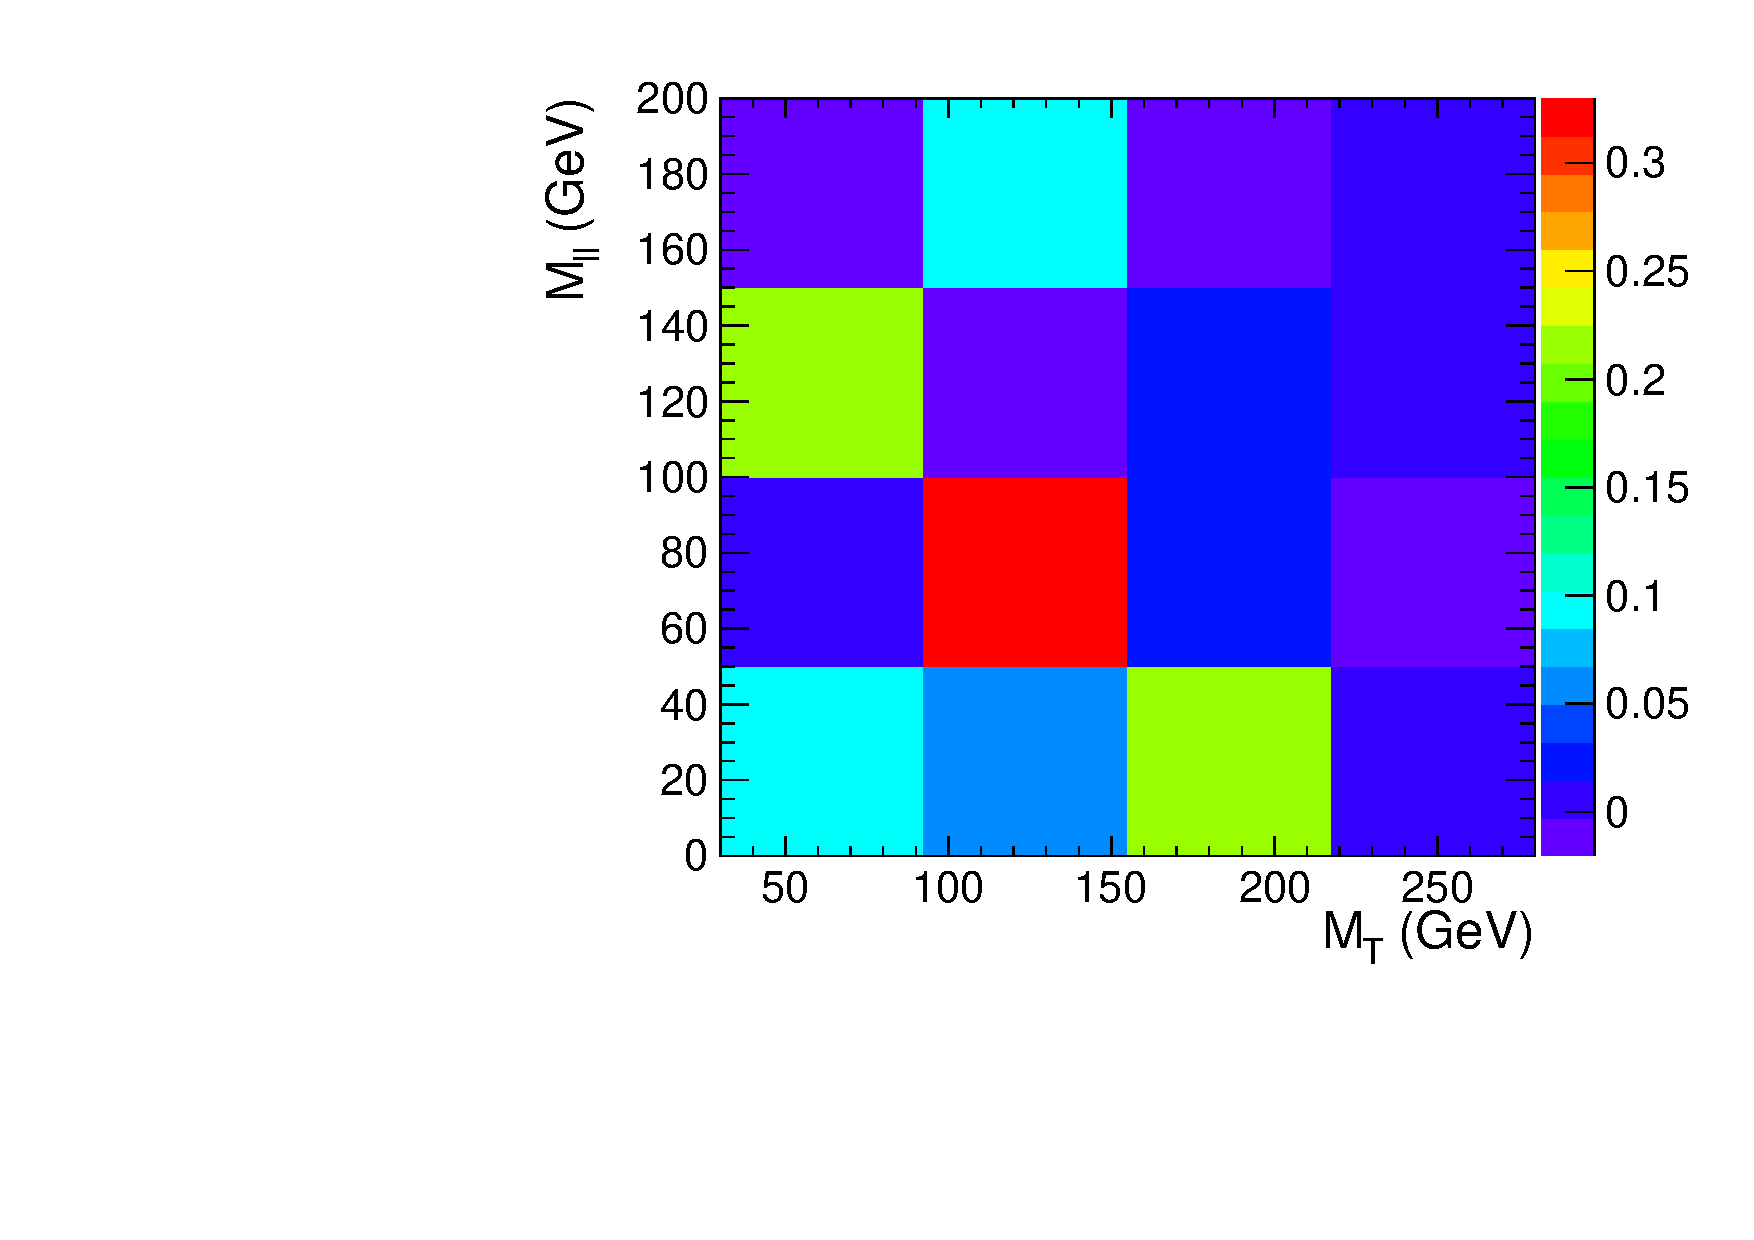
\includegraphics[width=.35\textwidth]{figures/templates/Wjets_2D_mH125_2j_of.pdf}
	}
	\subfigure[Wjets statistical uncertainty]{
	\centering
	\label{subfig:template_Wjetserr_125}
		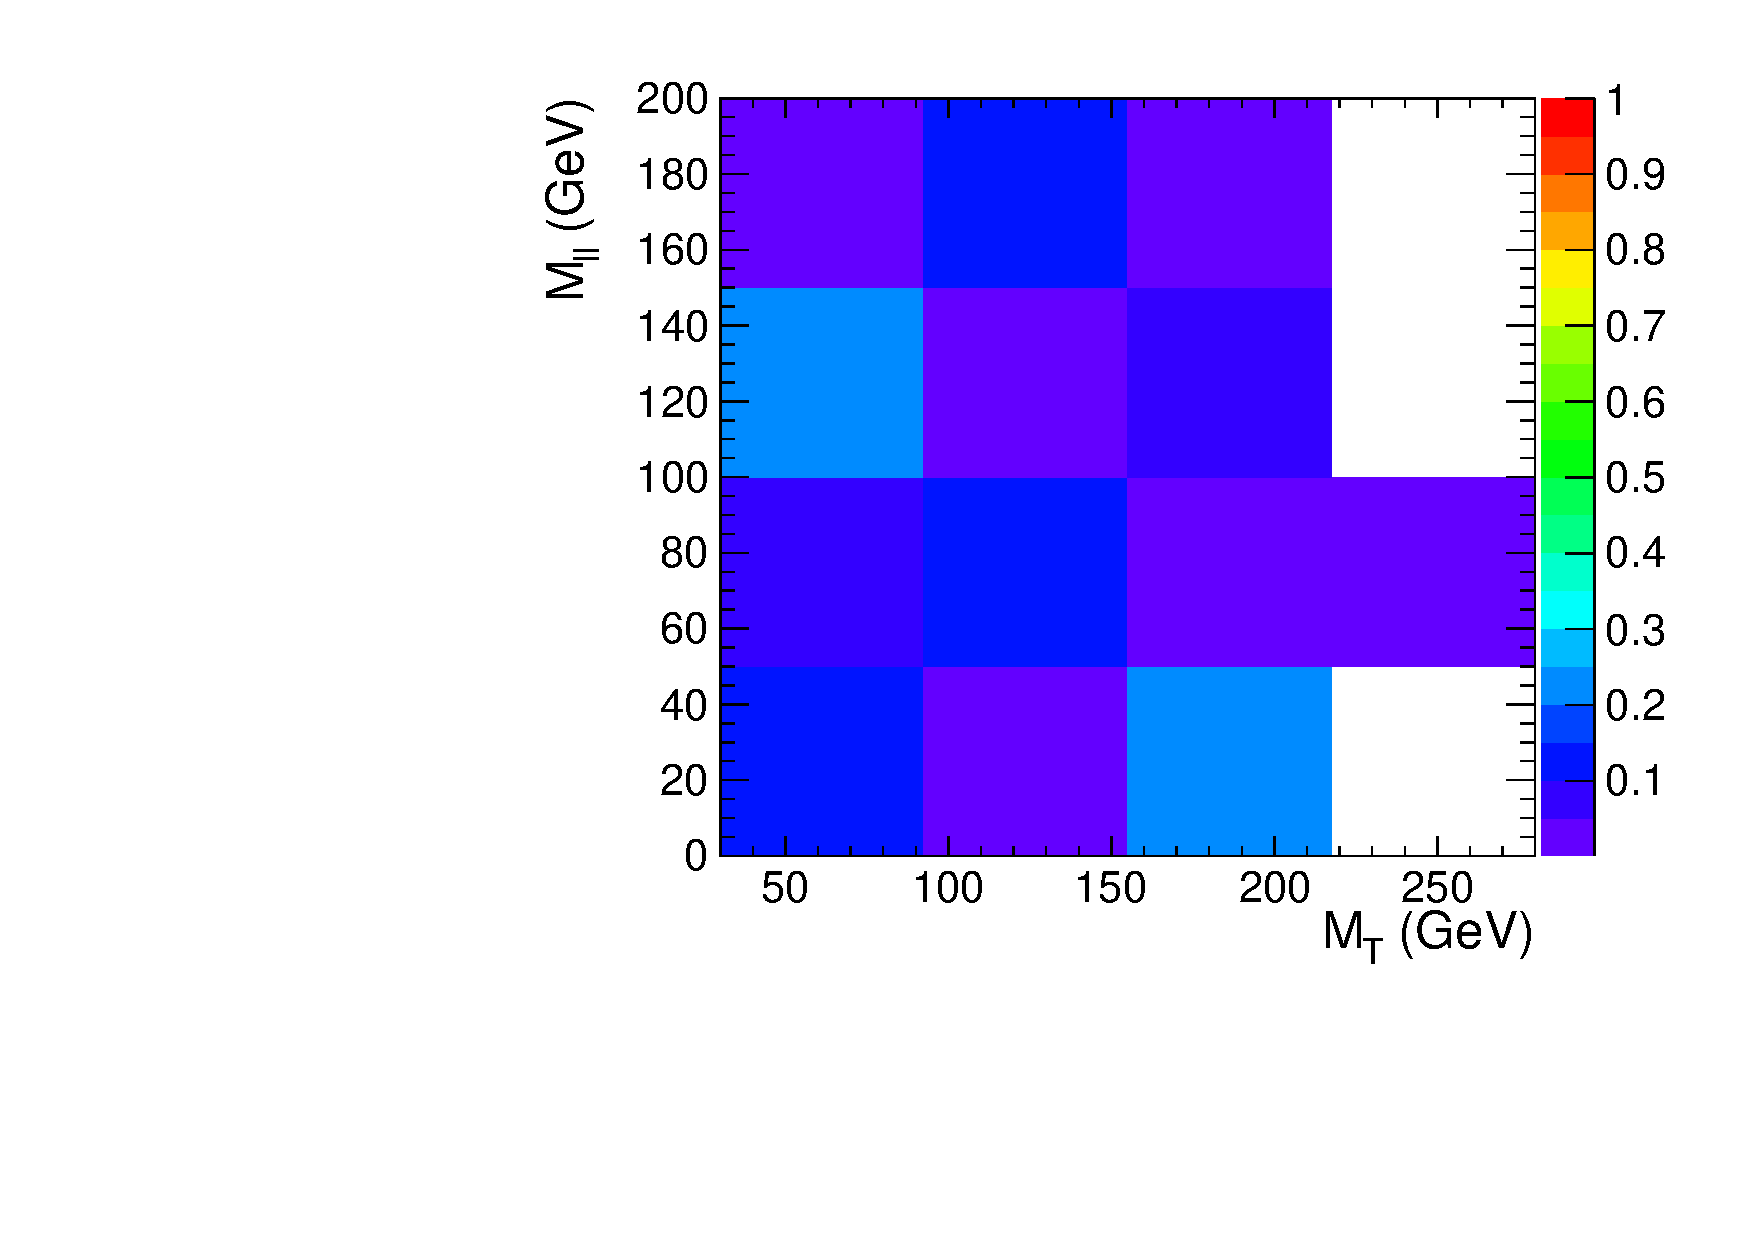
\includegraphics[width=.35\textwidth]{figures/templates/Wjetserr_2D_mH125_2j_of.pdf}
	}
	
	%
	\centering
	\subfigure[Top]{
	\centering
	\label{subfig:template_Top_125}
		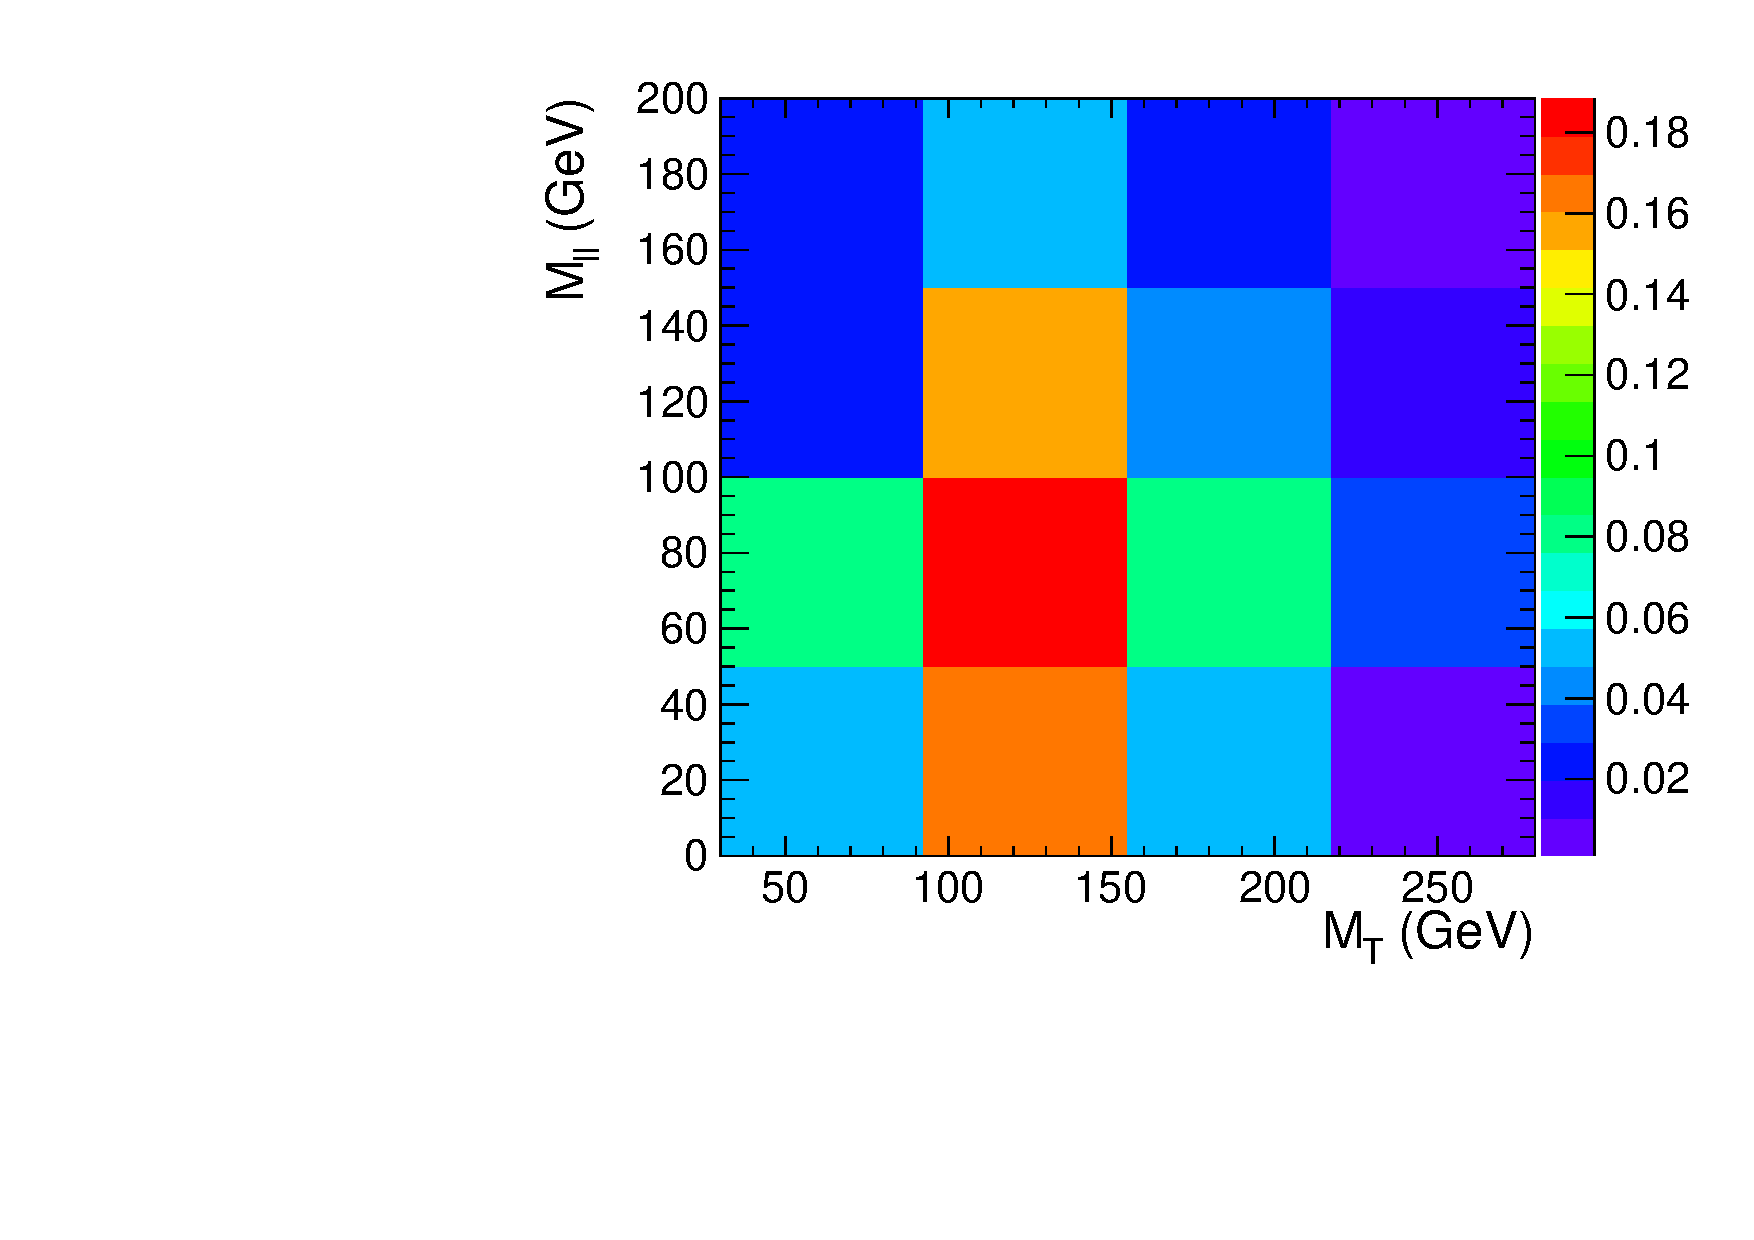
\includegraphics[width=.35\textwidth]{figures/templates/Top_2D_mH125_2j_of.pdf}
	}
	\subfigure[Top statistical uncertainty]{
	\centering
	\label{subfig:template_Toperr_125}
		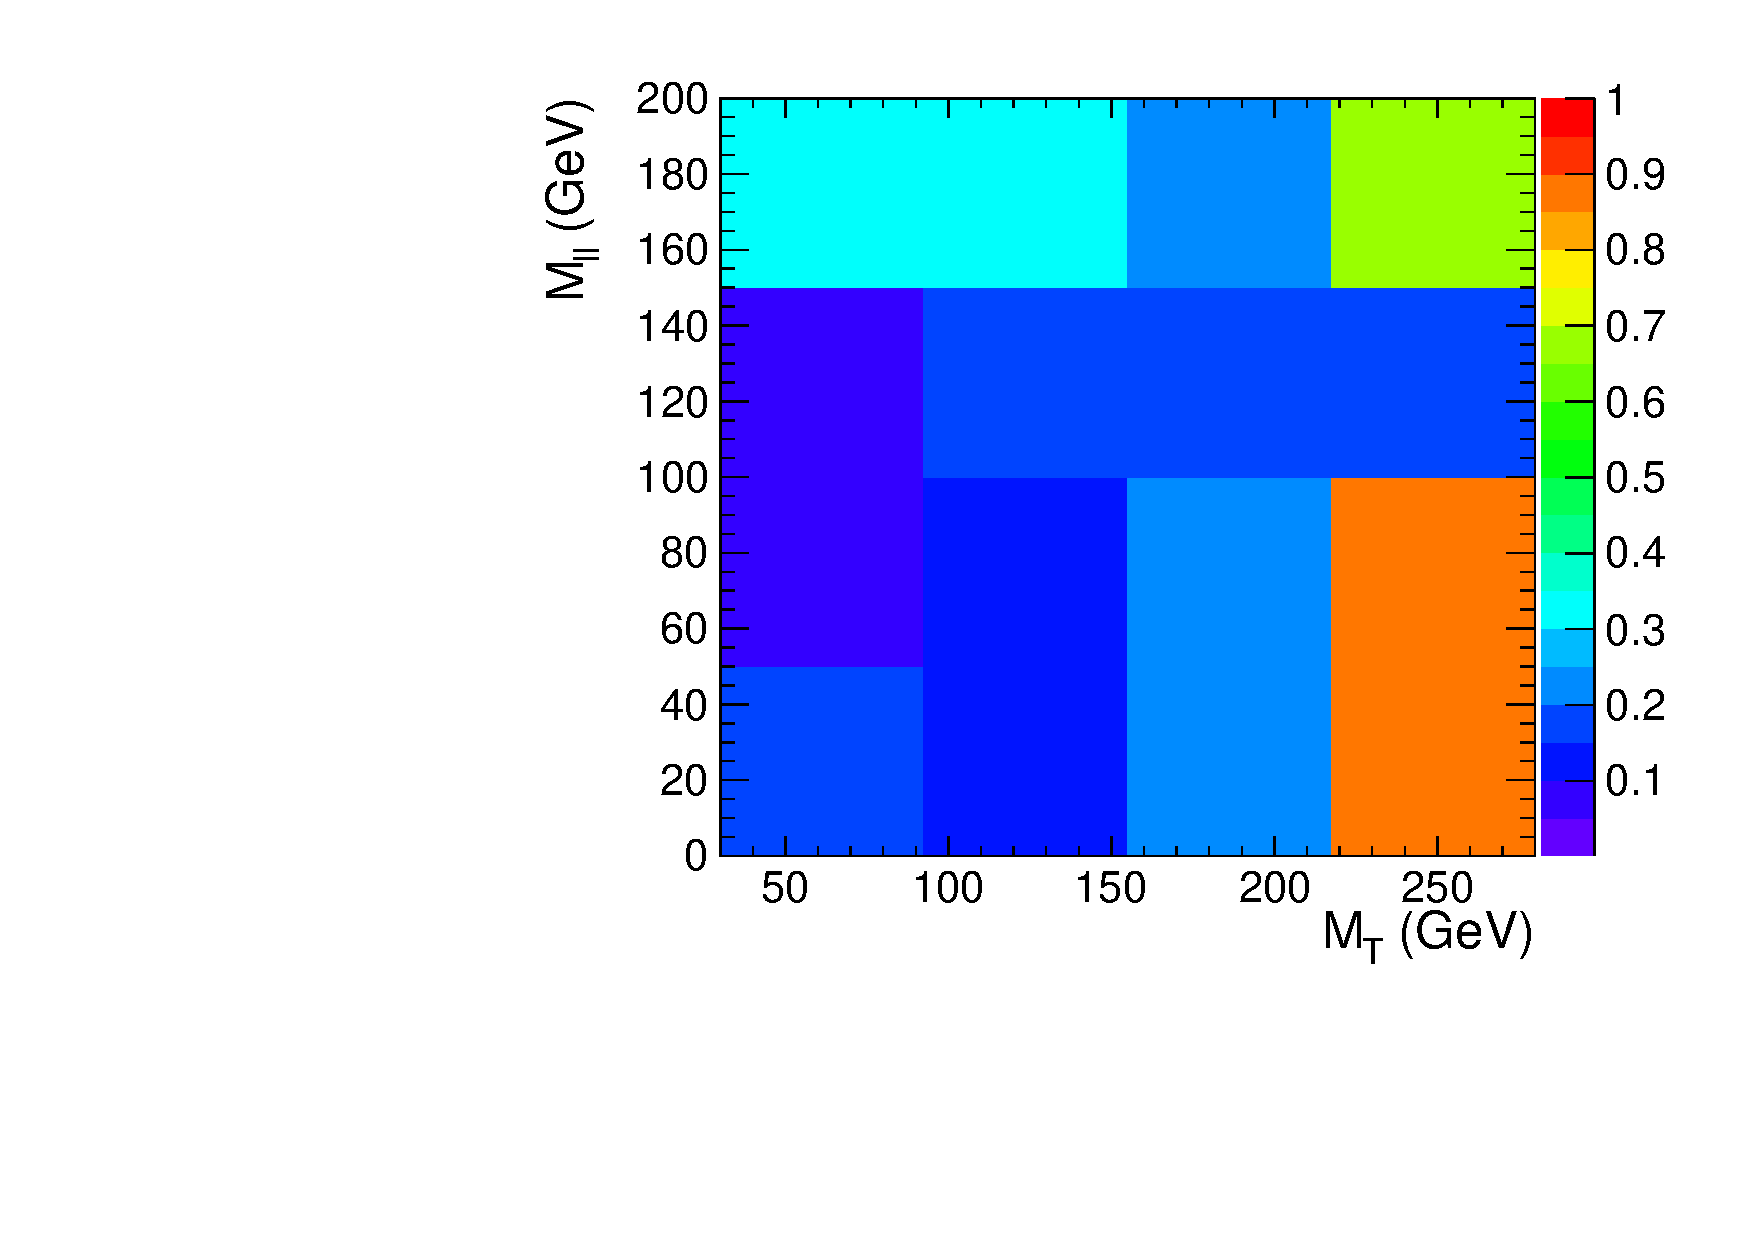
\includegraphics[width=.35\textwidth]{figures/templates/Toperr_2D_mH125_2j_of.pdf}
	}

	%
	\centering
	\subfigure[VV]{
	\centering
	\label{subfig:template_VV_125}
		\includegraphics[width=.35\textwidth]{figures/templates/VV_2D_mH125_2j_of.pdf}
	}
	\subfigure[VV statistical uncertainty]{
	\centering
	\label{subfig:template_VVerr_125}
		\includegraphics[width=.35\textwidth]{figures/templates/VVerr_2D_mH125_2j_of.pdf}
	}

	\caption{2D templates at \mHi = 125 \GeV in VBF channel.} 
	\label{fig:templates_125_vbf_2}

\end{figure}

\begin{figure}[!hbtp]
	
	%
	\centering
	\subfigure[Zjets]{
	\centering
	\label{subfig:template_Zjets_125}
		\includegraphics[width=.35\textwidth]{figures/templates/Zjets_2D_mH125_2j_of.pdf}
	}
	\subfigure[Zjets statistical uncertainty]{
	\centering
	\label{subfig:template_Zjetserr_125}
		\includegraphics[width=.35\textwidth]{figures/templates/Zjetserr_2D_mH125_2j_of.pdf}
	}

	%
%	\centering
%	\subfigure[Wgamma]{
%	\centering
%	\label{subfig:template_Wgamma_125}
%		\includegraphics[width=.35\textwidth]{figures/templates/Wgamma_2D_mH125_2j_of.pdf}
%	}
%	\subfigure[Wgamma statistical uncertainty]{
%	\centering
%	\label{subfig:template_Wgammaerr_125}
%		\includegraphics[width=.35\textwidth]{figures/templates/Wgammaerr_2D_mH125_2j_of.pdf}
%	}

	\caption{2D templates at \mHi = 125 \GeV in VBF channel.} 
	\label{fig:templates_125_vbf_3}

\end{figure} 

\begin{figure}[!hbtp]
	
	%
	\centering
	\subfigure[Stacked unrolled template linear]{
	\centering
	\label{subfig:template_unroll_stack_lin}
		\includegraphics[width=.45\textwidth]{figures/templates/2D_mH125_2j_of_stack_lin.pdf}
	}
	\subfigure[Overlaid unrolled template linear]{
	\centering
	\label{subfig:template_unroll_overlay_lin}
		\includegraphics[width=.45\textwidth]{figures/templates/2D_mH125_2j_of_overlay_lin.pdf}
	}

	%
	\centering
	\subfigure[Stacked unrolled template in log scale]{
	\centering
	\label{subfig:template_unroll_stack_log}
		\includegraphics[width=.45\textwidth]{figures/templates/2D_mH125_2j_of_stack_log.pdf}
	}
	\subfigure[Overlaid unrolled template in log scale]{
	\centering
	\label{subfig:template_unroll_overlay_log}
		\includegraphics[width=.45\textwidth]{figures/templates/2D_mH125_2j_of_overlay_log.pdf}
	}

	\caption{Unrolled templates at \mHi = 125 \GeV in VBF channel.} 
	\label{fig:templates_125_vbf_unroll}

\end{figure} 

\newpage
%%% mH=600 VBF 
\begin{figure}[!hbtp]
	
	%
	\centering
	\subfigure[Signal]{
	\centering
	\label{subfig:template_signal_600}
		\includegraphics[width=.35\textwidth]{figures/templates/sig_2D_mH600_2j_of.pdf}
	}
	\subfigure[Signal statistical uncertainty]{
	\centering
	\label{subfig:template_signalerr_600}
		\includegraphics[width=.35\textwidth]{figures/templates/sigerr_2D_mH600_2j_of.pdf}
	}
	
	%
	\centering
	\subfigure[qqWW]{
	\centering
	\label{subfig:template_qqWW_600}
		\includegraphics[width=.35\textwidth]{figures/templates/qqWW_2D_mH600_2j_of.pdf}
	}
	\subfigure[qqWW statistical uncertainty]{
	\centering
	\label{subfig:template_qqWWerr_600}
		\includegraphics[width=.35\textwidth]{figures/templates/qqWWerr_2D_mH600_2j_of.pdf}
	}

	%
	\centering
	\subfigure[ggWW]{
	\centering
	\label{subfig:template_ggWW_600}
		\includegraphics[width=.35\textwidth]{figures/templates/ggWW_2D_mH600_2j_of.pdf}
	}
	\subfigure[ggWW statistical uncertainty]{
	\centering
	\label{subfig:template_ggWWerr_600}
		\includegraphics[width=.35\textwidth]{figures/templates/ggWWerr_2D_mH600_2j_of.pdf}
	}

	\caption{2D templates at \mHi = 600 \GeV in 0 jet bin} 
	\label{fig:templates_600_vbf_1}

\end{figure}

\begin{figure}[!hbtp]
	
	%
	\centering
	\subfigure[Wjets]{
	\centering
	\label{subfig:template_Wjets_600}
		\includegraphics[width=.35\textwidth]{figures/templates/Wjets_2D_mH600_2j_of.pdf}
	}
	\subfigure[Wjets statistical uncertainty]{
	\centering
	\label{subfig:template_Wjetserr_600}
		\includegraphics[width=.35\textwidth]{figures/templates/Wjetserr_2D_mH600_2j_of.pdf}
	}
	
	%
	\centering
	\subfigure[Top]{
	\centering
	\label{subfig:template_Top_600}
		\includegraphics[width=.35\textwidth]{figures/templates/Top_2D_mH600_2j_of.pdf}
	}
	\subfigure[Top statistical uncertainty]{
	\centering
	\label{subfig:template_Toperr_600}
		\includegraphics[width=.35\textwidth]{figures/templates/Toperr_2D_mH600_2j_of.pdf}
	}

	%
	\centering
	\subfigure[VV]{
	\centering
	\label{subfig:template_VV_600}
		\includegraphics[width=.35\textwidth]{figures/templates/VV_2D_mH600_2j_of.pdf}
	}
	\subfigure[VV statistical uncertainty]{
	\centering
	\label{subfig:template_VVerr_600}
		\includegraphics[width=.35\textwidth]{figures/templates/VVerr_2D_mH600_2j_of.pdf}
	}

	\caption{2D templates at \mHi = 600 \GeV in VBF channel.} 
	\label{fig:templates_600_vbf_2}

\end{figure}

\begin{figure}[!hbtp]
	
	%
	\centering
	\subfigure[Zjets]{
	\centering
	\label{subfig:template_Zjets_600}
		\includegraphics[width=.35\textwidth]{figures/templates/Zjets_2D_mH600_2j_of.pdf}
	}
	\subfigure[Zjets statistical uncertainty]{
	\centering
	\label{subfig:template_Zjetserr_600}
		\includegraphics[width=.35\textwidth]{figures/templates/Zjetserr_2D_mH600_2j_of.pdf}
	}

	%
%	\centering
%	\subfigure[Wgamma]{
%	\centering
%	\label{subfig:template_Wgamma_600}
%		\includegraphics[width=.35\textwidth]{figures/templates/Wgamma_2D_mH600_2j_of.pdf}
%	}
%	\subfigure[Wgamma statistical uncertainty]{
%	\centering
%	\label{subfig:template_Wgammaerr_600}
%		\includegraphics[width=.35\textwidth]{figures/templates/Wgammaerr_2D_mH600_2j_of.pdf}
%	}

	\caption{2D templates at \mHi = 600 \GeV in VBF channel.} 
	\label{fig:templates_600_vbf_3}

\end{figure} 

\begin{figure}[!hbtp]
	
	%
	\centering
	\subfigure[Stacked unrolled template linear]{
	\centering
	\label{subfig:template_unroll_stack_lin}
		\includegraphics[width=.45\textwidth]{figures/templates/2D_mH600_2j_of_stack_lin.pdf}
	}
	\subfigure[Overlaid unrolled template linear]{
	\centering
	\label{subfig:template_unroll_overlay_lin}
		\includegraphics[width=.45\textwidth]{figures/templates/2D_mH600_2j_of_overlay_lin.pdf}
	}

	%
	\centering
	\subfigure[Stacked unrolled template in log scale]{
	\centering
	\label{subfig:template_unroll_stack_log}
		\includegraphics[width=.45\textwidth]{figures/templates/2D_mH600_2j_of_stack_log.pdf}
	}
	\subfigure[Overlaid unrolled template in log scale]{
	\centering
	\label{subfig:template_unroll_overlay_log}
		\includegraphics[width=.45\textwidth]{figures/templates/2D_mH600_2j_of_overlay_log.pdf}
	}

	\caption{Unrolled templates at \mHi = 600 \GeV in VBF channel.} 
	\label{fig:templates_600_vbf_unroll}

\end{figure} 

